%-----------------------------------------------------------PREAMBLE-----------------------------------------------------------%
\documentclass{cup_PSRM}

\usepackage[T1]{fontenc}
\usepackage{amsfonts, amsmath, amssymb}
\usepackage{authblk}
\usepackage{multirow}
\usepackage{epsfig}
\usepackage{subfigure}
\usepackage{subfloat}
\usepackage{graphicx}
\usepackage{lscape}
\usepackage{amsmath}
\usepackage{amssymb}
\usepackage{gensymb}


\usepackage{booktabs}
\usepackage{longtable}

\usepackage{verbatim, rotating, paralist}
\usepackage{enumerate}
% \usepackage{natbib}
\usepackage{pdfsync}
\usepackage{latexsym}
% \usepackage{amsthm}

\usepackage{stmaryrd}
\usepackage{dsfont}
\usepackage{hyperref}
\usepackage{bbm}
\usepackage{mathtools}

\usepackage{parskip}
\usepackage{anysize, indentfirst, setspace}
% \usepackage[right=1.75cm, left=1.75cm, top=2.25cm, bottom=2.25cm]{geometry}
\usepackage{tikz}
\usetikzlibrary{arrows,shapes,backgrounds,positioning,patterns,decorations.pathreplacing}
\usepackage{epigraph}
\usepackage{csquotes}

\usepackage{appendix}
\usepackage{lipsum} % for dummy text
\usepackage{enumitem}
\usepackage{rotating}




\setlist{nosep}

\renewcommand{\topfraction}{.85}
\renewcommand{\bottomfraction}{.7}
\renewcommand{\textfraction}{.15}
\renewcommand{\floatpagefraction}{.66}
\renewcommand{\dbltopfraction}{.66}
\renewcommand{\dblfloatpagefraction}{.66}





%\usepackage{setspace} % load setspace before footmisc
%\usepackage{footmisc}
%\setlength{\footnotesep}{\baselineskip} %use 1.67\baselineskip for a double space


%\renewcommand{\footnotelayout}{\doublespacing}

% \makeatletter
% \renewcommand\footnotesize{%
%    \@setfontsize\normalsize\@ixpt{11}%
%    \abovedisplayskip 8\p@ \@plus2\p@ \@minus4\p@
%    \abovedisplayshortskip \z@ \@plus\p@
%    \belowdisplayshortskip 4\p@ \@plus2\p@ \@minus2\p@
%    \def\@listi{\leftmargin\leftmargini
%                \topsep 4\p@ \@plus2\p@ \@minus2\p@
%                \parsep 2\p@ \@plus\p@ \@minus\p@
%                \itemsep \parsep}%
%    \belowdisplayskip \abovedisplayskip
% }
% \makeatother

\journalname{Draft Submission to Political Science Research and Methods}
\journalcopy{The European Political Science Association, 2016}
\fpage{X}
\lpage{XXX}
\journalvolume{X}
\journalissue{X}
\doinumber{doi:10.1017/psrm.XXXX.XX}

\addbibresource{precinct.bib}


%-----------------------------------BEGIN DOCUMENT-------------------------------------%
\begin{document}


\doublespacing
\setlength{\parindent}{0.45in}
\setlength{\parskip}{.0in}




%---------------------------------------TITLE PAGE---------------------------------%
\title{Polling Place Changes and Political Participation:\\ Evidence from North Carolina Presidential Elections, 2008-2016\footnote{Authors are listed alphabetically; all contributed equally.  We thank Dan Smith and Ken Mayer for helpful feedback on an earlier version and we thank Henry Goldberg for fabulous research assistance and for tracking down what we often thought was unobtainable.}}

\author{Joshua D. Clinton\footnote{ \footnotesize  Abby and Jon Winkelried Professor, Professor of Political Science and Co-Director of the Center for the Study of Democratic Institutions, Vanderbilt University; josh.clinton@vanderbilt.edu. }  \hspace*{.175in} Nick Eubank\footnote{\footnotesize Assistant (Research) Professor, Duke University; nick.eubank@duke.edu. }  \hspace*{.175in} Adriane Fresh\footnote{\footnotesize Assistant Professor, Duke University; adriane.fresh@duke.edu. }\hspace*{.175in}  Michael E. Shepherd\footnote{\footnotesize Graduate Student, Department of Political Science, Vanderbilt University; michael.e.shepherd@vanderbilt.edu. }}


\date{Version: \today  \\ \vspace*{.3in} }


\maketitle
\vspace{.1in}




%-------------------------------------------------------------------ABTRACT-----------------------------------------------------------------%
% Still horrible
\begin{abstract}
\bigskip
\small
\noindent How do changes in Election Day polling place locations affect voter turnout? We study the behavior of more than 2 million eligible voters across three closely-contested presidential elections (2008-2016) in the swing state of North Carolina. Leveraging within-voter variation in polling place location change over time, we demonstrate that polling place changes reduce Election Day voting on average statewide. However, this effect is almost completely offset by substitution into early voting, suggesting that voters, on average, respond to a change in their polling place by choosing to vote early. While there is heterogeneity in these effects by the distance of the polling place change and the race of the affected voter, the fully offsetting substitution into early voting still obtains.  We theorize this is because voters whose polling places change location receive notification mailers, offsetting search costs and priming them to think about the election before election day, driving early voting.
\end{abstract}

\vspace{.2in}
\textbf{Keywords}: Voting; Political Participation; Election Administration


%------------------------------------------ INTRODUCTION ---------------------------------------%


\noindent  The nature and quality of democracy is closely connected to questions of which members of the polity are able to participate in the electoral process \citep{keyssar2009right}. Indeed, work on the impact of felon disenfranchisement laws \citep{gerber2017does}, voter identification laws \citep{grimmer2017comment, highton2017voter, citrin2014effects}, early voting policies \citep{fullmer2015,burden2017complicated}, registration windows \citep{burden2014election, hanmer2009discount, leighley2013votes}, and variation in voting machines, operating hours and waiting times \citep{herron2016precinct, herron2015precinct, highton2006long, stewart2015waiting, pettigrew2017racial} have all demonstrated the importance of election administration decisions for political participation and electoral outcomes.

The decision of where to locate polling places represents another such routine election administration decision that impacts whether and how voters are able to participate in the electoral process.  Insofar as voters are sensitive to changes in the costs of voting --- as ample theory suggests \citep{downs1957, wolfinger1980votes, powell1986american, highton2004voter} --- changing where voters vote is likely to impact voter turnout by: creating confusion among affected voters, introducing search costs to find the new polling place, affecting how long it takes to travel to the polls \citep{brady2011turning, amos2017reprecincting}, and disrupting voting habits \citep{brody1977life, plutzer2002becoming, gerber2003voting}.

In this paper, we test how voter turnout responds to costs that result from changes in the location of Election Day polling places.  We do so by assembling a  balanced panel of more than 2 million eligible voters from the North Carolina voter rolls across three presidential elections --- 2008, 2012 and 2016.  For each election, we geolocate every voter and every polling place to identify whether a voter experienced a polling place change and to measure the resulting change in the voter's travel time to their polling place.  We further measure whether a voter votes, and how they cast their ballot --- e.g. on Election Day or in-person early.\footnote{We refer in the remainder of the paper to ``early voting'' in place of ``in-person early voting'' and distinguish this from early voting by mail (i.e. absentee voting) which we term ``mail-in voting.''}  Using this data, we leverage within-\emph{individual} variation to estimate the state-wide average effect of a polling place change on voter turnout.  By employing a comprehensive set of fixed effects and fixed effect interactions, we account for many potential confounders to an unbiased estimation of this relationship --- these include the individual propensity to vote, common features of elections that may affect turnout, trends in turnout (and turnout by \emph{mode}) for voters of different races, and county-specific trends in factors like early voting availability.  We therefore substantially limit the scope for unobserved heterogeneity to confound our results.

We find that the effect of changes in polling place locations are more complex than existing theory on the depressive turnout consequences of increased voting costs would predict. Amongst our balanced panel of non-movers, polling place changes decrease Election Day voting by about    -0.7\unskip~percentage points on average, but this effect is nearly perfectly offset by an \emph{increase} in in-person early voting.   Furthermore, when we allow our effects to vary by important characteristics of voters, like race, we find the same off-setting, although weaker, pattern amongst non-whites. Overall, our results indicate that voters respond to changes in the costs associated with voting on Election Day by \emph{substituting} into an alternative mode of voting, \emph{not} by forgoing casting a ballot. Although this substitution appears somewhat puzzling, we theorize that this occurs because voters whose polling places change location receive notification mailers, priming them to think about the election before election day, driving early voting.\footnote{Although we can provide some evidence to support this contention, we contend that a full test of this theoretical proposal should occur in future work.}

Our results are consistent in a number of ways with the pathbreaking work of \cite{brady2011turning} on the consequences of polling place changes.  Analyzing the California 2003 gubernatorial recall election, the authors find that voters whose precincts were consolidated --- and thus whose assigned polling place changed --- were 1.85\% less likely to vote. The authors also find that polling-place voting declined by 3\%, but that this was \emph{partially} offset by a 1.2\% increase in mail-in voting. In addition to an intrinsic effect of a polling place change, the authors find that the effect varies with the change in distance to the poll.  Like \cite{brady2011turning}, we find a decline in Election Day voting, substitution between voting modes, as well as a greater decline in turnout amongst those whose polling places were moved further from their homes.

Crucially however, our results also differ from those of \cite{brady2011turning}, and subsequent important studies by \cite{amos2017reprecincting} and \cite{yoder2018}, in several important ways. First, we do not find evidence of an overall decrease in turnout on the scale found by these authors nor that we can distinguish from zero; rather, we find that Election Day voting declines modestly (   -0.7\unskip~percentage points) and early voting nearly perfectly offsets those declines.  Furthermore, we find that while those moved further from their polling place substitute more between modes, that substitution is once again entirely offsetting.

Moreover, in the spirit of ``normal'' scientific advancement, our analysis allows us to substantially improve our confidence in the the findings of earlier work \citep{brady2011turning}, while providing additional nuance to those results. First, and most obviously, our improvements in data and research design substantially narrow the space for our results to be contaminated by unobserved heterogeneity, improving our confidence that the quantities we estimate (and to the extent that those results are similar to existing results, that those results too) are indicative of true causal effects. Second, because we are theory testing (and not generating new theory based on new results), our analysis is not susceptible to the sharpshooter fallacy.\footnote{To be clear, this is not a critique of \cite{brady2011turning} --- \emph{all} papers that propose new theory on the basis of new empirical results are susceptible to the sharpshooter fallacy (the possibility that a theory generated to rationalize an empirical finding is essentially just overfitting noise); indeed, it is for precisely this reason that explicit theory testing is a necessary part of the scientific enterprise.}

Third and finally, the scope of our analysis also allows us to probe the generalizability of existing findings and to help contextualize them more broadly. Where \cite{brady2011turning} examine effects of polling place changes in a single gubernatorial recall election in a single county (Los Angeles), we examine behavioral patterns across an entire state and multiple presidential elections. Insofar as we are concerned about how polling place changes may impact state and national election outcomes by changing turnout --- a real possibility in the pivotal and closely contested swing state of North Carolina --- the cross-county heterogeneity we find makes it clear that it is important to look beyond a single locality to identify the average statewide effect, an effect that has never previously been estimated.

Our analysis also documents considerable county-level variation in the estimated effects of polling place changes in North Carolina. We show that while there is no \emph{systematic} evidence that polling place changes impact overall turnout --- there are as many counties where the estimated effect is positive as there are counties where the effect is negative. An analysis focused on a single county might therefore erroneously conclude that voters are \emph{systematically} influenced by polling place changes, while when contextualized in a state-wide analysis, this interpretation appears unlikely to be correct. This highlights the importance of examining more than a single election administrative unit (e.g. a county), especially when endogenous case selection is a possibility.\footnote{Selecting a case precisely because one expects a particular, and not necessarily representative, electoral effect.}  Indeed, the variation that we document should be of interest to the entire election administration and election forensics literatures where studies of voters in a \emph{single} unit where election administration decisions such as polling places are made (typically the county) are the norm rather than the exception \citep{dyck2005distance, gimpel2003political, haspel2005location, cantoni2016, amos2017reprecincting}.

Of course, even this study is a study of a single state.  But in addition to being a state whose electoral outcomes are of intrinsic interest to both state-level and national politics, as we discuss in detail in this paper, our ability to study the universe of counties (each of which makes their own polling place location decisions) under North Carolina's state-wide election administration institutions provides a perspective on cross-county variation (and thus interpretation of county-specific estimates) that is simply unavailable in single-county studies.  Furthermore, that the negative turnout effects found by \cite{yoder2018} in North Carolina, specifically, differ from ours may further highlight the dangers of inferring state-wide effects from a limited sample of counties, as key analyses the author performs utilize a limited sample of North Carolina counties.\footnote{\cite{yoder2018} also considers primary elections in some of his analyses, which are another possible explanation for the differing results.  We strongly emphasize that when \cite{yoder2018} replicates our analyses with the full sample of counties and only presidential elections, he obtains our identical results.}

Our paper further contributes with a number of key measurement and research design improvements.  Our panel data allow us to eliminate movers from our analysis --- that is, those who move far enough that they fully \emph{select into} polling place changes, and who must therefore search for their new polling place location \emph{regardless} of whether the polling place that they will vote at is in the same location as a previous election.  Our data also allow us to estimate changes in \emph{travel time} to the polls, rather than simply geometric ``as-the-crow-flies'' distance, which may obscure important road density and traffic variation that impact turnout.  Our balanced panel across three elections allows us to employ a research design with extensive fixed effects and fixed effect interactions to eliminate potential confounders, which improves on much of the literature on this topic.

The lack of an overall impact on turnout is perhaps surprising in light of theoretical claims about how costs impact turnout.  However, we elaborate a number rationales for the state-wide substitution effects that we find.  First, North Carolina voters receive an official county mailer advising them whenever their polling place changes, and providing early voting information.  As well as counteracting confusion, these mailers may operate like get-out-the-vote primes \citep{arceneaux2009mobilized}.  And indeed the magnitude of the substitution we find is highly consistent with turnout estimates from this literature \citep{gerber2000effects}.

The offsetting substitution we find also accords with findings on how voters respond to a disruption in their voting habit \citep{meredith2011convenience}.  If voters are risk averse and value voting, they may substitute into a less risky mode of voting where they have the time to search for information and overcome costs and errors rather than risk not casting a ballot at all.  While some have suggested that the availability of early voting decreases turnout \citep{burden2014early}, our findings suggest that the availability of early voting may help mitigate the negative effects of polling place changes on turnout by allowing voters more time to find an alternative polling place.  Of course, this is a suggestive interpretation as it is impossible to know the overall consequences if early voting were not an option at all.  Together these explanations rationalize our results, but merit further investigation in other settings and with other designs to understand the ways in which costs imposed on voting can be moderated.







%--------------------------------------- CONTEXT ---------------------------------------%
\section{The Potential Effects of Polling Place Changes}\label{section_context}

\noindent  The large literature on political participation has long argued that \emph{any} imposition of costs is likely to reduce participation \citep{downs1957, wolfinger1980votes, powell1986american, highton2004voter} and the behavioral expectations of the impact of polling place changes are therefore exceptionally clear --- changes in location should depress turnout by increasing the costs of voting.  First, the simple fact of a moved polling place may be costly to voters even if there is no change in the time needed to travel to the poll because of psychological costs --- confusion and habit disruption --- that voters must overcome to cast a ballot \citep{brady2011turning, amos2017reprecincting}.

Second, changes to polling place locations almost always alter how long it takes most voters to travel to cast a ballot.  While confusion and habit disruption unequivocally increase voting costs, changing travel times do not \citep{brady2011turning, dyck2005distance, gimpel2003political, haspel2005location,cantoni2016, amos2017reprecincting}.  We might expect that those whose polling places are moved farther away may forgo casting a ballot due to the increased cost of traveling to the polls, while those whose polling places are moved closer may be \emph{more} likely to turnout since their costs have been reduced. Though this effect may b further moderated by where people work, run errands, etc. in addition to where people live.  The relative impact of increased as compared to decreased travel times, as well as travel costs relative to \emph{per se} costs is theoretically unclear.

We may also expect differences in the relative ability of different groups to overcome the costs associated with polling place changes.  Although, racial differences in participation have declined since the 1980s \citep{leighley2013votes,fraga2016candidates}, voters with fewer material resources --- lower income and minority voters, for example --- might be less able to overcome increased costs to voting \citep{verba1995voice}.\footnote{The effect of fewer resources may also be true for movers.  However, as we note in the subsequent section, movers are unique in how they effectively select to experience a polling place change, which, for most of them, makes it observationally infeasible to distinguish the effect of moving from the effect of a polling place changing.} Alternatively, historical experiences with disenfranchisement, or other group norms \citep{anollnorms}, may differentially motivate non-white voters to overcome the costs imposed by polling place changes to cast their ballot.

The literature on costs and participation would conclude that increasing the cost of casting a ballot should result in lower turnout.  But the election administration policies of North Carolina may also exacerbate or counteract some of the increased costs associated with polling place changes.  Most notably, voters have a choice between voting on Election Day or early. Voters who choose to vote early can vote at any early voting location in the county with no excuse.  There is variation in the number of early voting locations between counties which we control for in our analyses, but every county has to have at least one early voting location open for 100 total hours prior to Election Day.\footnote{Mail-in voting is rare, but also possible.}

If voters are risk averse, or value their vote highly, moving a polling place may cause voters to vote early in response.  Prior work has indeed found evidence that voters shift between modes of voting rather than forgo casting a ballot when there are changes in the procedures for a particular mode of voting \citep{michelson2012effect,malhotra2011text}.  Voters worried about their ability to vote in a new polling place may choose to vote early rather than risk the uncertainties of dealing with a new polling place on Election Day.  While some have argued that convenience voting may decrease turnout \citep{burden2014early} (while others have found the opposite \citep{gerbergreenhill2013}), \emph{for voters who are forced to find and vote at a new polling place because their polling place was changed}, the ability of voters to vote early may provide them with the incentive and opportunity to vote early in response.

Another important feature of the North Carolina electoral landscape is the fact that County Board of Elections send out an informational mailer to all voters affected by a polling place change.  The mailer provides voters with the address of their new polling place and links to websites with further information about early voting. An example of a mailer from Wake County is provided in Appendix B. These mailers in theory help offset the search costs involved with finding the new polling place, locate the county's early voting location, as well as effectively providing a reminder to vote.  In fact, voting primes are well-known to affect turnout \citep{gerber2000effects, gerber2008social}, and prior work suggests that reminders by election administrators can moderate the negative consequences of certain election reforms \citep{bergman2011changing}.\footnote{But see \cite{meredith2014voting} on the ineffectiveness of information provided to ex-felons eligible to vote.}  Insofar as these mailers reduce the cost of gathering information on early voting by identifying its existence and providing web information, existing research suggests that they may also help induce voters to change their method of voting to the convenience method \citep{monroesylvesterVoteByMail,votingmessagesmilitary}.



%----------------------------------------- DATA -----------------------------------------%
\section{Data on Voters, Votes, and Polling Places}\label{section_data}

\noindent  To identify the effects of polling place changes on voters in North Carolina we collect individual-level data on every voter from the official state voter rolls between 2008 and 2016.  We supplement this data with information on precinct boundaries and the location of nearly every polling place in the state for each election.  Our choice of North Carolina is in part a function of the unique availability of comprehensive voter and polling place information, but it is also motivated by the ability to study the effect of polling place changes at the state level over several closely contested and highly-salient elections with national implications.

Our individual-level dataset contains demographics, polling place assignments, and voting histories for     2,350,731\unskip~unique voters collected from snapshots of the North Carolina Voter Roll provided by North Carolina State Board of Election (NCSBE) between 2008 and 2016.\footnote{More specifically, data was downloaded by the authors from the NCSBE data site \url{http://dl.ncsbe.gov/index.html} in November of 2017. Data for the 2016 presidential election comes from the November 8th, 2016 snapshot, data for the 2012 presidential election comes from the November 6th, 2012 snapshot, and data for the 2008 presidential election comes from the November 4th, 2008 snapshot.} The voter file contains information on voter registration status, party registration, race, gender, and age which are then paired with records from the North Carolina State Board of Elections on how each voter voted (e.g., Election Day, mail-in, in-person early), if at all, in the three presidential elections.

We focus our analysis on what we refer to as our ``balanced panel'' of    4,434,125\unskip~voter-year observations where voters must be eligible to vote\footnote{These eligible individuals are voters with voter status of ``Active,'' ``Temporary,'' or ``Inactive.'' ``Inactive'' is a label used by the NCSBE for voters who have failed to vote in several past elections, and who \emph{will be} (but are not yet) eligible for removal if they continue to not vote.} in both 2008 and 2012.  Two years of eligibility are required as a first time voter cannot, by definition, experience a \emph{change} in polling place location. Note, however, that as the ability to vote in 2012 may impact subsequent eligibility to vote, subsetting for voters who are \emph{also} eligible in 2016 could potentially create bias due to selection after treatment.\footnote{Reducing our sample only those active in 2008 would not reduce any post-treatment bias.  If a voter is active in 2008 and were to experience a polling place change between 2008 and 2012, that cannot make the voter \emph{inactive} in the voter roll in 2012 \emph{even if} they fail to vote in 2012.  If the voter is active in 2008, the soonest they can become inactive is 2016.  There is no mechanism that can result in ineligibility/inactive status in 2012 as a result of a polling place change that takes place between 2008 and 2012.}  That we have a balanced panel allows us to track the behavior of \emph{the same voters} over time to ensure that the effects we identify are a consequence of polling place changes rather than compositional changes in voters being analyzed.\footnote{Our panel covers two different partisan regimes of election administration appointments --- changes made in 2012 were made by local administrators appointed by a Democratic administration and changes made in 2016 were made by Republican appointees --- but there is actually little theoretical reason to expect that polling place changes made under each of these regimes would produce different \emph{overall} turnout effects. If the effect of a polling place change is driven by the confusion and habit disruption of a \emph{per se} change, the partisanship of administrators should not matter.  If these \emph{per se} costs can be offset by an increase or decrease in travel times to the polls, then local election administrators' choices might increase turnout for those moved closer to polling places, while decrease turnout for those moved further away.  Yet, unless there is important heterogeneity in how partisan voters respond to a change, we would expect the depressive effect of being moved further from a polling place to offset the increased turnout of those moved closer.  In evaluating heterogeneity in turnout effects by race (as well as income and age in an Appendix D), we implicitly evaluate this potential heterogeneity. (In Appendix M we also show that while for some outcomes there are small differences in turnout under different partisan regimes, these are both extremely small (approximately half of one percentage point) and unfortunately confounded by the fact that there are other differences between the years besides partisan regime that may have played a role in participation.)}.



To identify the location of voters' residences in our panel, we geocode voter addresses using the \url{geocod.io} geocoding service\footnote{This generates a total of    4,253,361\unskip~voters who we can geocode in at least two sequential elections ---      95.9\unskip\% of  those possible.  The reasons for failed geo-codes --- e.g. typos in voter roll addresses --- are likely to be idiosyncratic and unrelated to turnout decisions.}, and we link voters to their precincts and Election Day polling places for the three presidential elections that we examine. Polling place locations were also geocoded using the \url{geocod.io} geocoding service and merged with shapefiles of election precinct boundaries (see Appendix L for details).  We also use this spatial information to exclude people from our analysis have moved. Focusing on the    2,350,731\unskip~unique individuals (     69.9\unskip\% of all geocoded, eligible voters with polling places) ensures that the effects of polling place changes we identify are a consequences of polling places being moved, rather than the movements of voters.

The one exception to our exclusion of movers are people who made relatively small moves where their new residence had, in the previous election, the same polling place assignment as their old residence.\footnote{To be as clear as possible, there are two general categories of people who move residences.  The first, are \emph{inter-precinct movers}, people for whom their new and their old residence are sufficiently far from one another that they are not voting in the same precinct --- that is, there is no possibility that such a person \emph{could have} used the same polling place were they not to have moved (and were their old polling place to have remained in the same location).  This is as compared to the second type of person --- \emph{within-precinct} movers (this moniker is effectively if not strictly true because precincts are not stable units over time) --- are people who move short enough distances such that \emph{were} their polling place to remain in the same location, they could use that same polling place (though that polling place may move).  Again, as noted above, we remove the first category of people from our analysis.  We strongly contend that it is not meaningful to discuss whether the polling place of such a person has moved.  Whether or not the location of such a mover's new polling place is the same as the last election, that polling place is \emph{always} going to be new to the person who moved.  Such inter-precinct movers will have to incur search costs to look up where their new polling place is regardless  of whether the polling place that is new to them is in the same location as it was in the last election.  We consider it unreasonable to consider that anyone would move and look up where a polling place was in a \emph{past} election rather than where it will be in the upcoming election.  Is is these within-precinct movers that we consider in Appendix O.} We do not analyze these movers in our primary analyses: it would be in appropriate to include them in analyses that include distance to polling places (because changes in the \emph{distance} to their polling place is not due only to administrative changes), and thus we also exclude them from analyses of the impact of polling place changes \emph{per se} to avoid compositional changes across analyses.  Crucially, we do examine the differential effect of polling place changes \emph{per se} for this population relative to non-movers separately in Appendix O.\footnote{Note that of the    1,012,077 movers in our data, only      115,500 of them moved to residences that share the same polling place assignments as their old residences, making this a relatively small subsample of all movers, and of our sample overall.}  As we describe in more detail in the appendix, our results demonstrate statistically significant heterogeneity for this population of movers.  Consistent with literatures noting the resource-differences of movers, these movers are slightly less likely to substitute and slightly less likely to turnout to voter overall when they have a polling place moved administratively.


%% TABLE: Our sample compared to voter roll-eligible voters
%%-----------------------------------------------------------------------------
\begin{table}[t!]\centering \small
\caption{Our Sample Compared to Voter Roll-Eligible Voters}\label{table_sample_comparison}
\vspace*{.055in}
\begin{tabular}{l c c }
\hline\hline\noalign{\smallskip}
	\multicolumn{1}{c}{Variable} & Our Balanced Panel & Voter Rolls \\
	\hline \noalign{\smallskip}
	$VotedAny$  &    0.80 &    0.72  \\
	$Movers$  & 0.00 &    0.31 \\
	$Age$&   57.02 &   50.49  \\
	$Female$&    0.55 &    0.57  \\
	$White$&    0.76 &    0.66  \\
	$NonWhite$&    0.24 &    0.35 \\
	$Republican$&    0.35 &     0.29  \\
	$Democrat$&    0.44 &     0.39  \\
	$\mathit{Unaffiliated}$&     0.21 &     0.23  \\
	\hline \noalign{\smallskip}
	Voter-Election Obs &      4,681,792 &     12,860,588 \\
		\noalign{\smallskip}\hline\hline\noalign{\smallskip}
	\multicolumn{3}{p{2.8in}}{\scriptsize{\emph{Notes:} The unit of analysis is the voter-election. Summary statistics are pooled means for 2012 and 2016 --- i.e. an individual voter enters once for 2012 and once for 2016. The Voter Rolls column includes voters who were eligible to vote in at least one of the three presidential elections in our sample.}}
\end{tabular}
\end{table}

Table \ref{table_sample_comparison} compares our panel to the set of all eligible voters according to the 2008-2016 voter rolls (additional summary statistics and details of data sources can be found in Appendix A).  Our panel restrictions alter our sample in predictable ways.  Our sample is on average more white, more partisan (i.e., more likely to include registered Republicans and Democrats) and older than the universe of eligible voters in the voter rolls.  These traits all correlate with political participation \citep{leighley2013votes}, and the turnout rate of our balanced panel is subsequently and unsurprisingly roughly 8 percentage points higher than the voter file.  However, scholarship on the relationship between voter mobility and voter turnout reassuringly finds estimated mobility effects that are roughly comparable to the turnout differences we observe between our panel and the voter roll \citep{squire1987residential,highton2000residential}.

Overall,           17\unskip\% of voters experienced a polling place change between 2008 and 2012 and            16\unskip\% experienced a change between 2012 and 2016. Polling place changes can arise for one of two reasons: the location of a given precinct's polling place may be moved, or else a change in a precinct's boundary can move a voter from one precinct to another.  Although most of the changes are due to re-precincting rather than adding or subtracting the number of polling places, by gathering data on both county-drawn precinct boundaries \emph{and} polling place locations, we are identify the consequences of either change.

In our analysis, we focus only on changes made between presidential elections (rather than between the current general election and the preceding general election). We do so for two reasons. First, we feel focusing only on presidential elections improves comparability in our panel. But second, and more importantly, in North Carolina nearly all (general) Election Day polling place changes take place in the immediate run-up to a presidential election. As such, there are almost no cases where a voter's Election Day polling place was changed between a presidential election and the subsequent mid-term, and so our variable for ``has voter's polling place changed since the last presidential election'' is nearly equivalent to ``has voter's polling place changed since the last general election.''

To illustrate the type of changes we examine, Figure~\ref{figure_map_charlotte_pp} presents maps of the location of Election Day polling places in 2008 and 2012 (a) relative to those in 2012 and 2016 (b) for Precinct 22 in central Charlotte.  Between 2008 and 2012, the polling place in Precinct 22 was moved to a Census block with a higher-than-average percentage of black residents (Census block groups are shaded in the background according to their racial composition in the 2010 Census, with darker shades indicating a higher percentage of black residents).  But in 2016, the location of the polling place was moved back to a part of the precinct with a higher percentage of white voters.  In addition to identifying the overall effect of such changes on turnout, we also use the richness of our data to examine whether voter characteristics such as race condition the effect.  To probe the robustness of the results to factors that may vary at the county level -- and to highlight inferential issues that can arise from focusing on a specific locality -- we also examine the effects of precinct changes for each county to determine if some counties have larger effects than others. In so doing, we correct for the problems caused by multiple testing \citet{Benjamini:2006gd}.

%  FIGURE: Example polling place location changes
%-------------------------------------------------------------------
\begin{figure}[t!]
	\begin{center}
	\caption{Polling places in Precinct \#22, Charlotte, Mecklenburg county}
		\small \vspace*{.05in}
		\smallskip
		(a) 2008 and 2012 (Democrats)  \hspace*{1.2in} (b) 2012 and 2016 (Republicans) \\
		\smallskip
				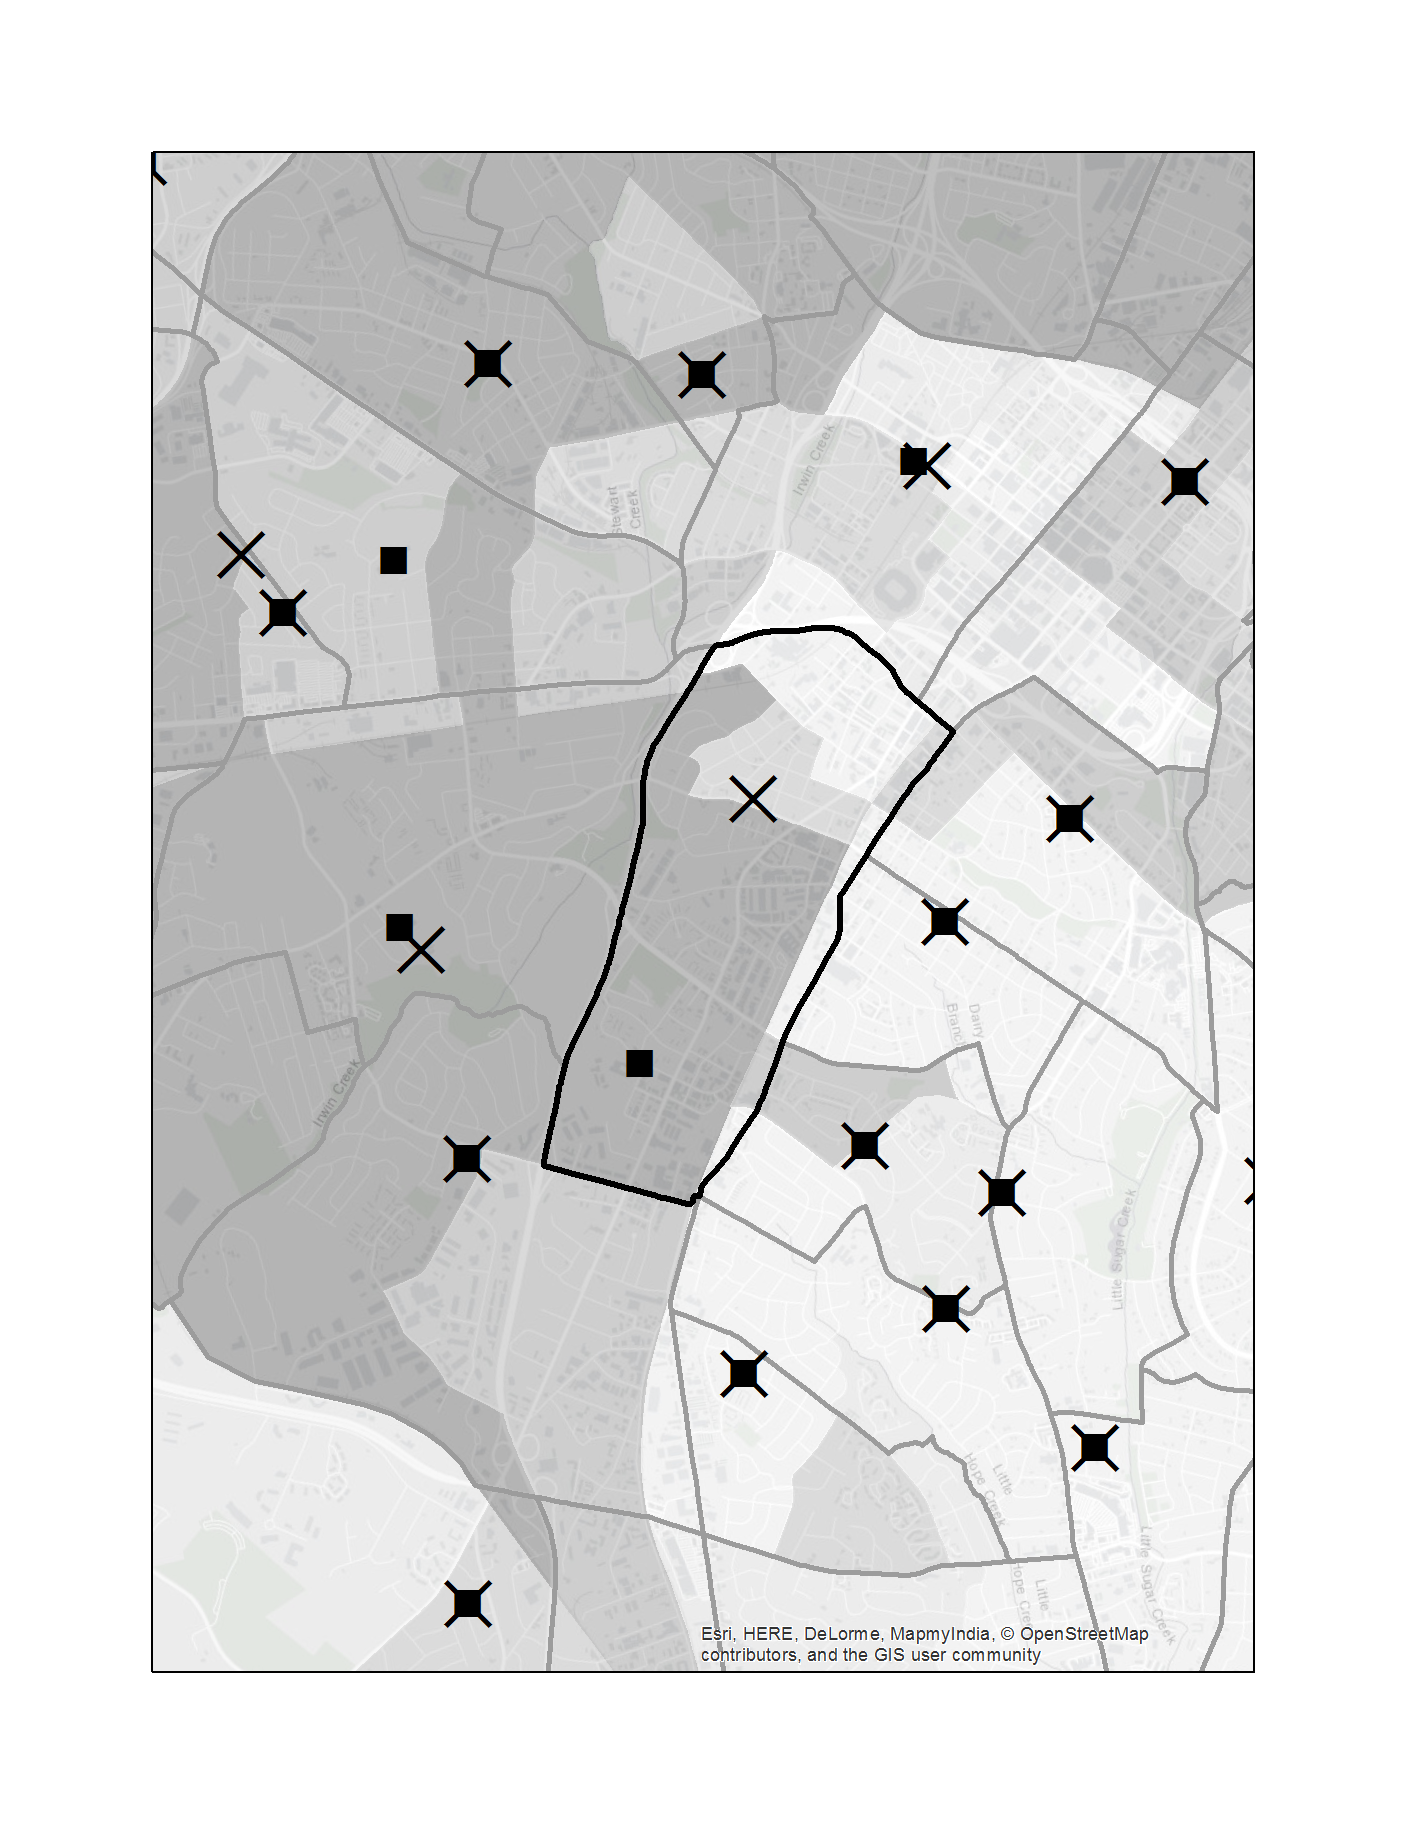
\includegraphics[ width=3in,  clip=true,  trim= 1.5in 2.45in 1.5in 2.45in ]{../../50_results_full/Map_Paper_Charlotte_PP_2008_2012.png} \hspace*{.1in}
				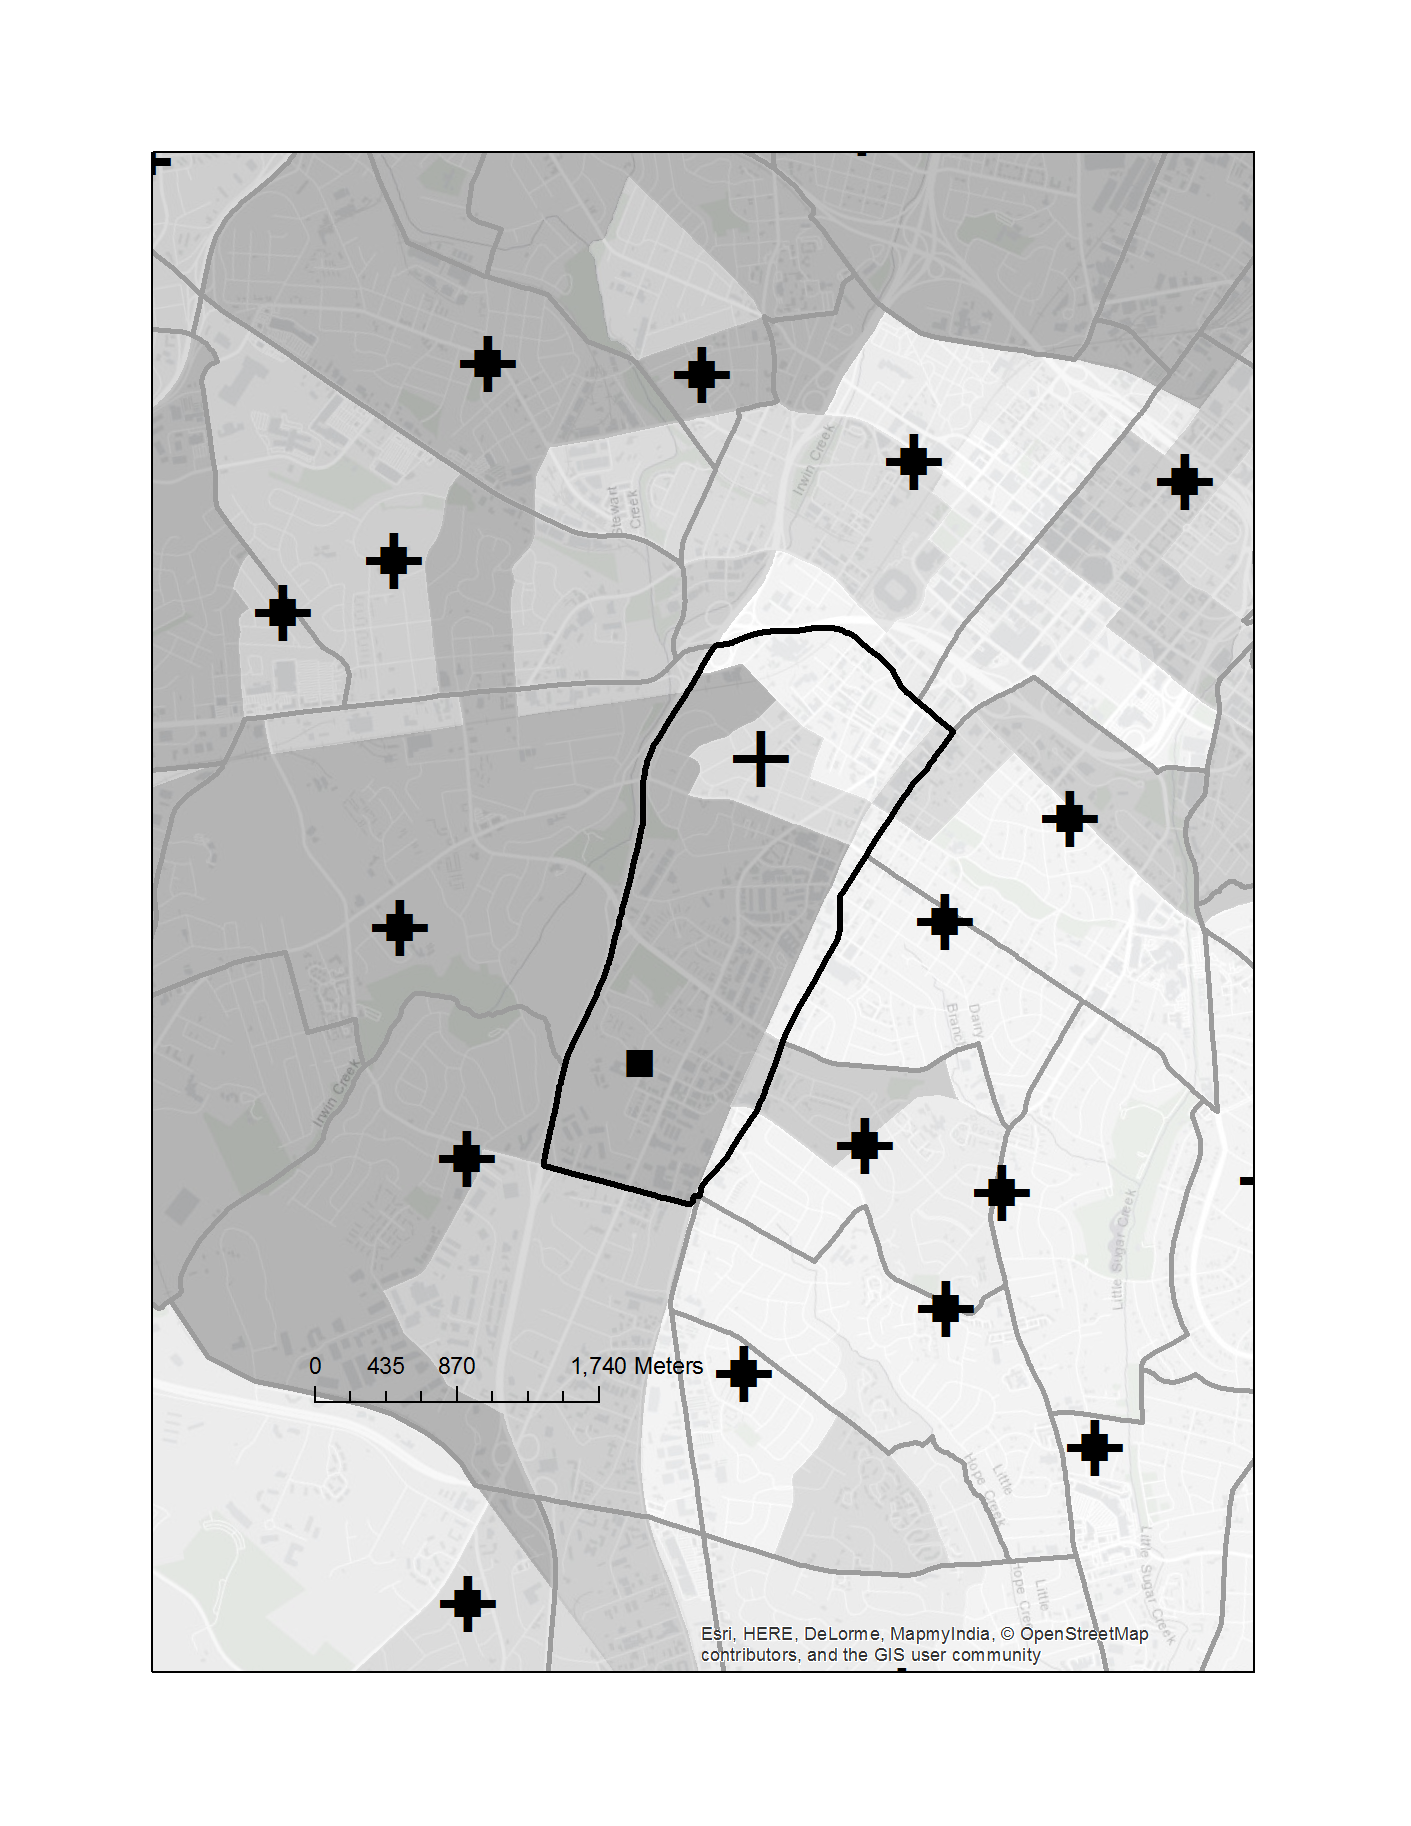
\includegraphics[ width=3in,  clip=true,  trim= 1.5in 2.45in 1.5in 2.45in ]{../../50_results_full/Map_Paper_Charlotte_PP_2012_2016.png} \\

				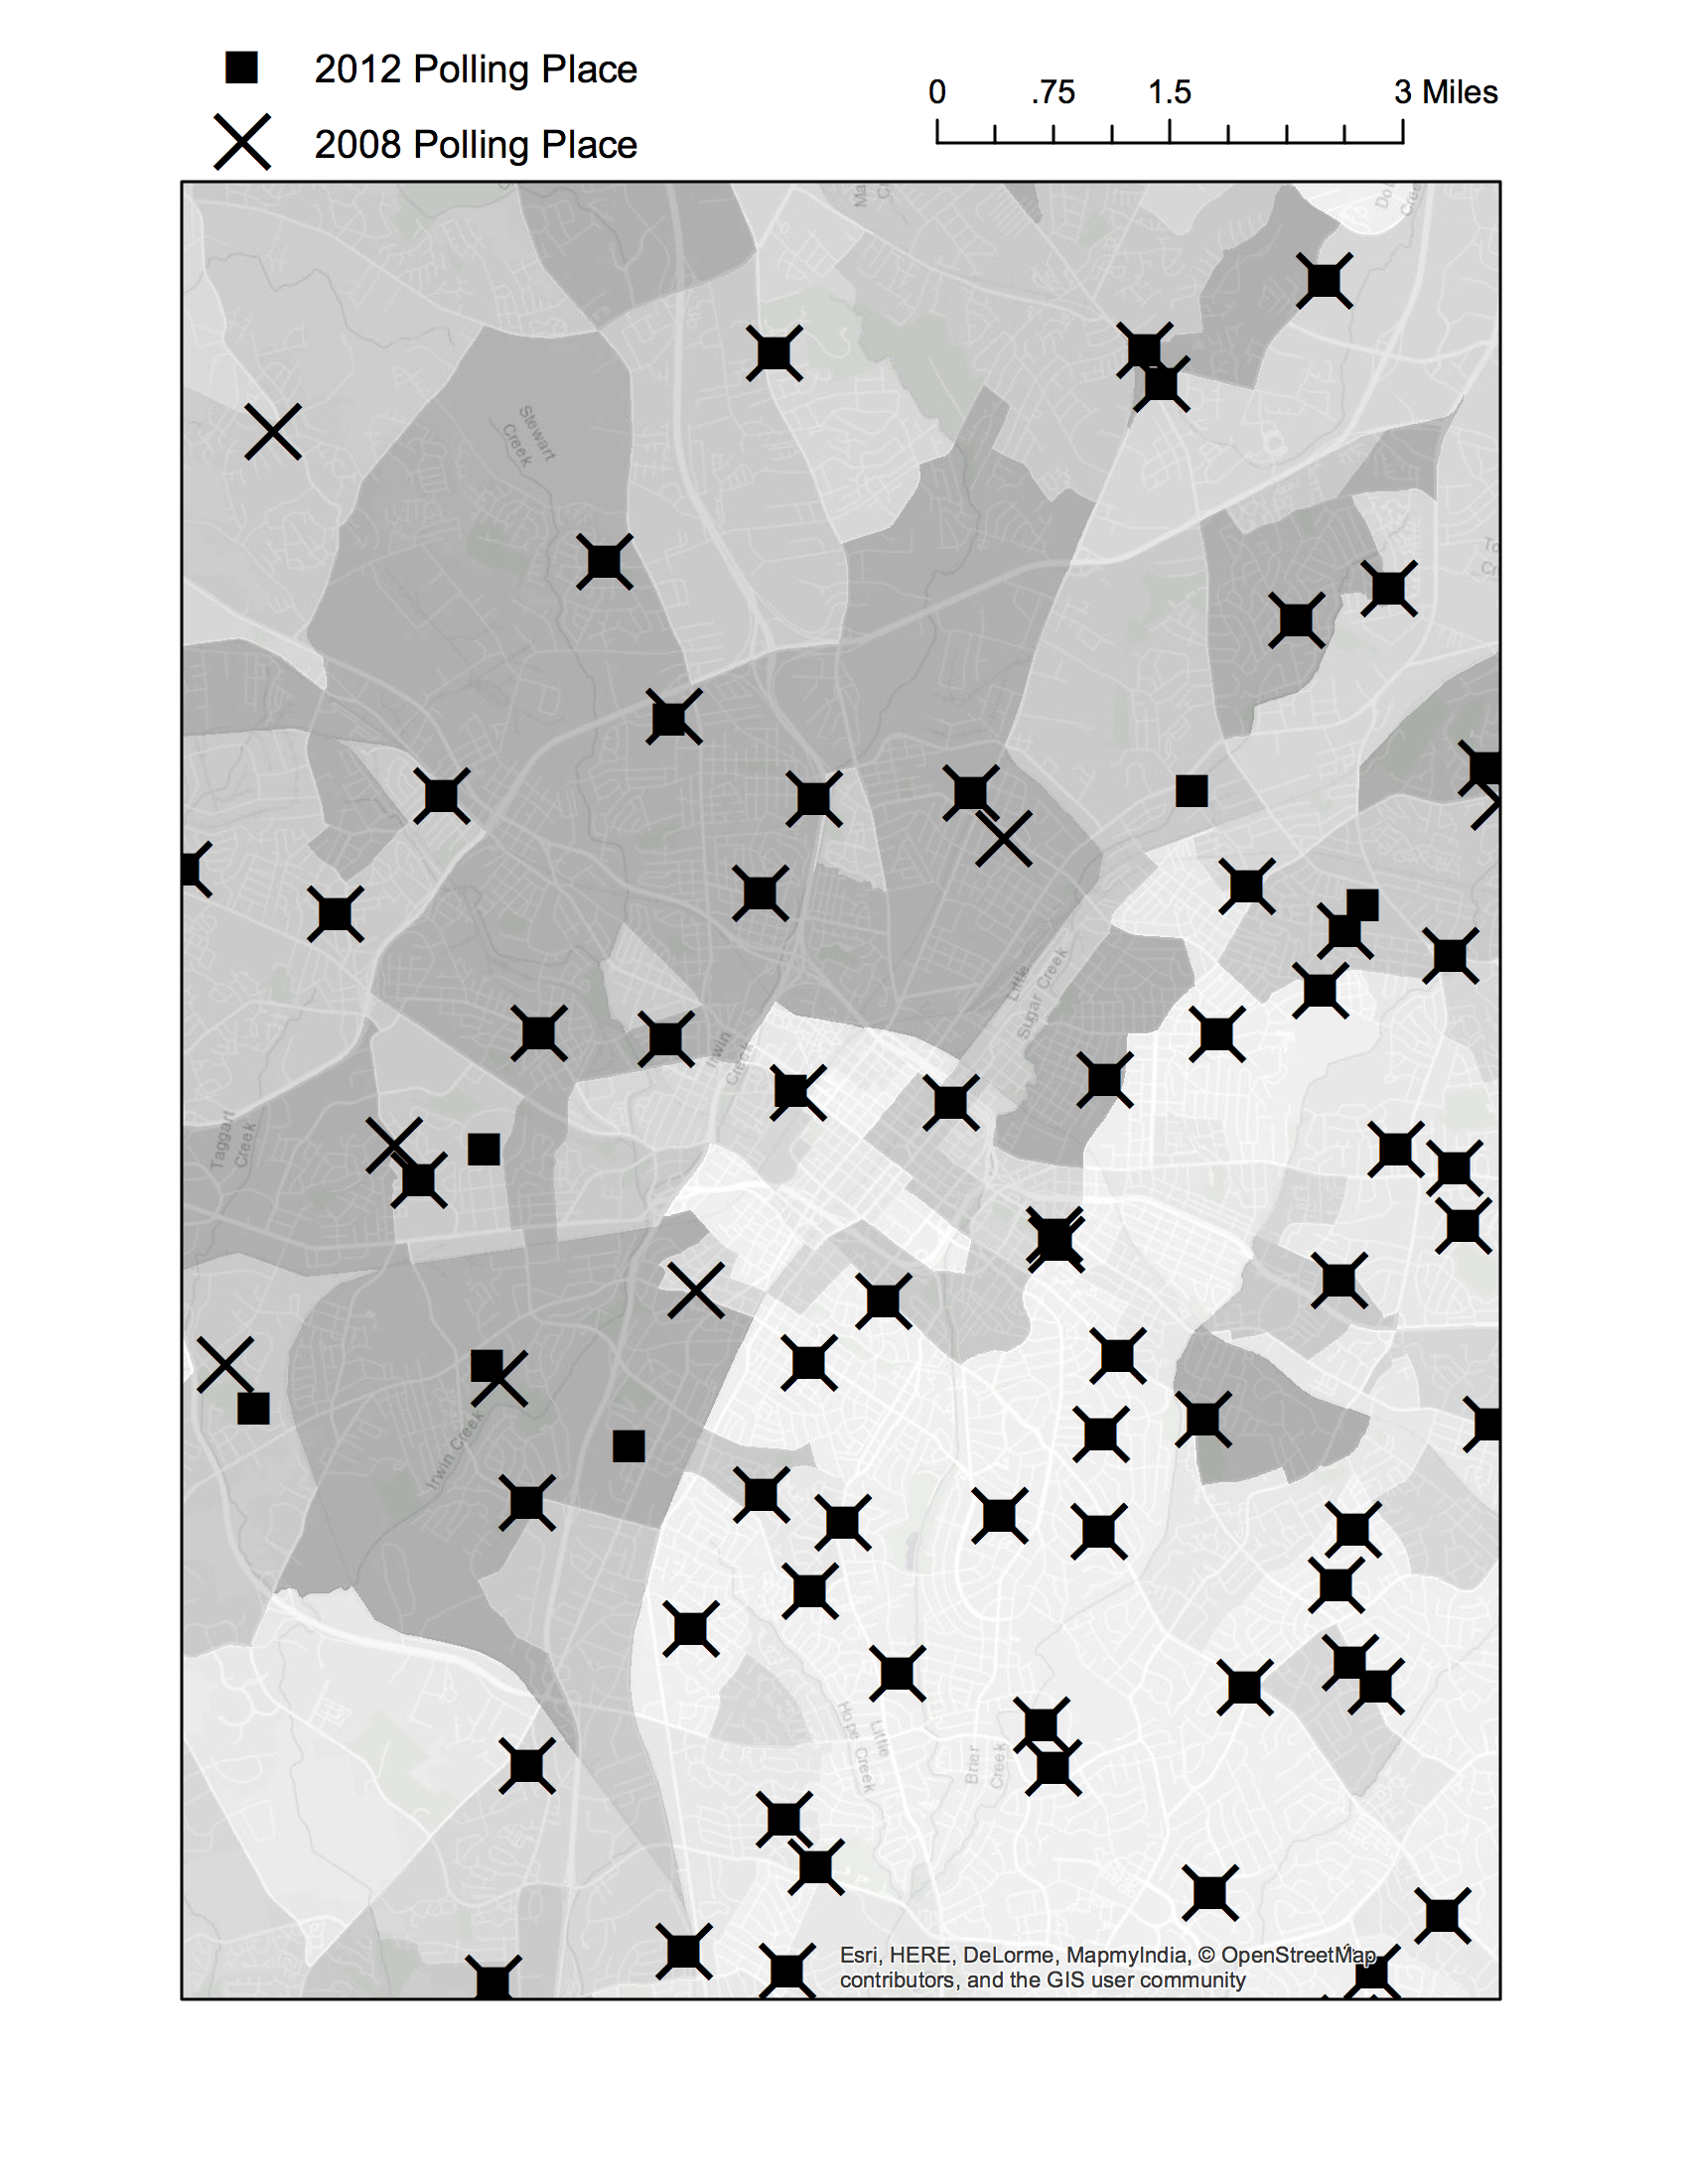
\includegraphics[ width=1.3in,  clip=true,  trim= 1.0in 10.13in 4.9in 0.5in ]{../../50_results_full/Map_Charlotte_PP_Legend_B.png}
				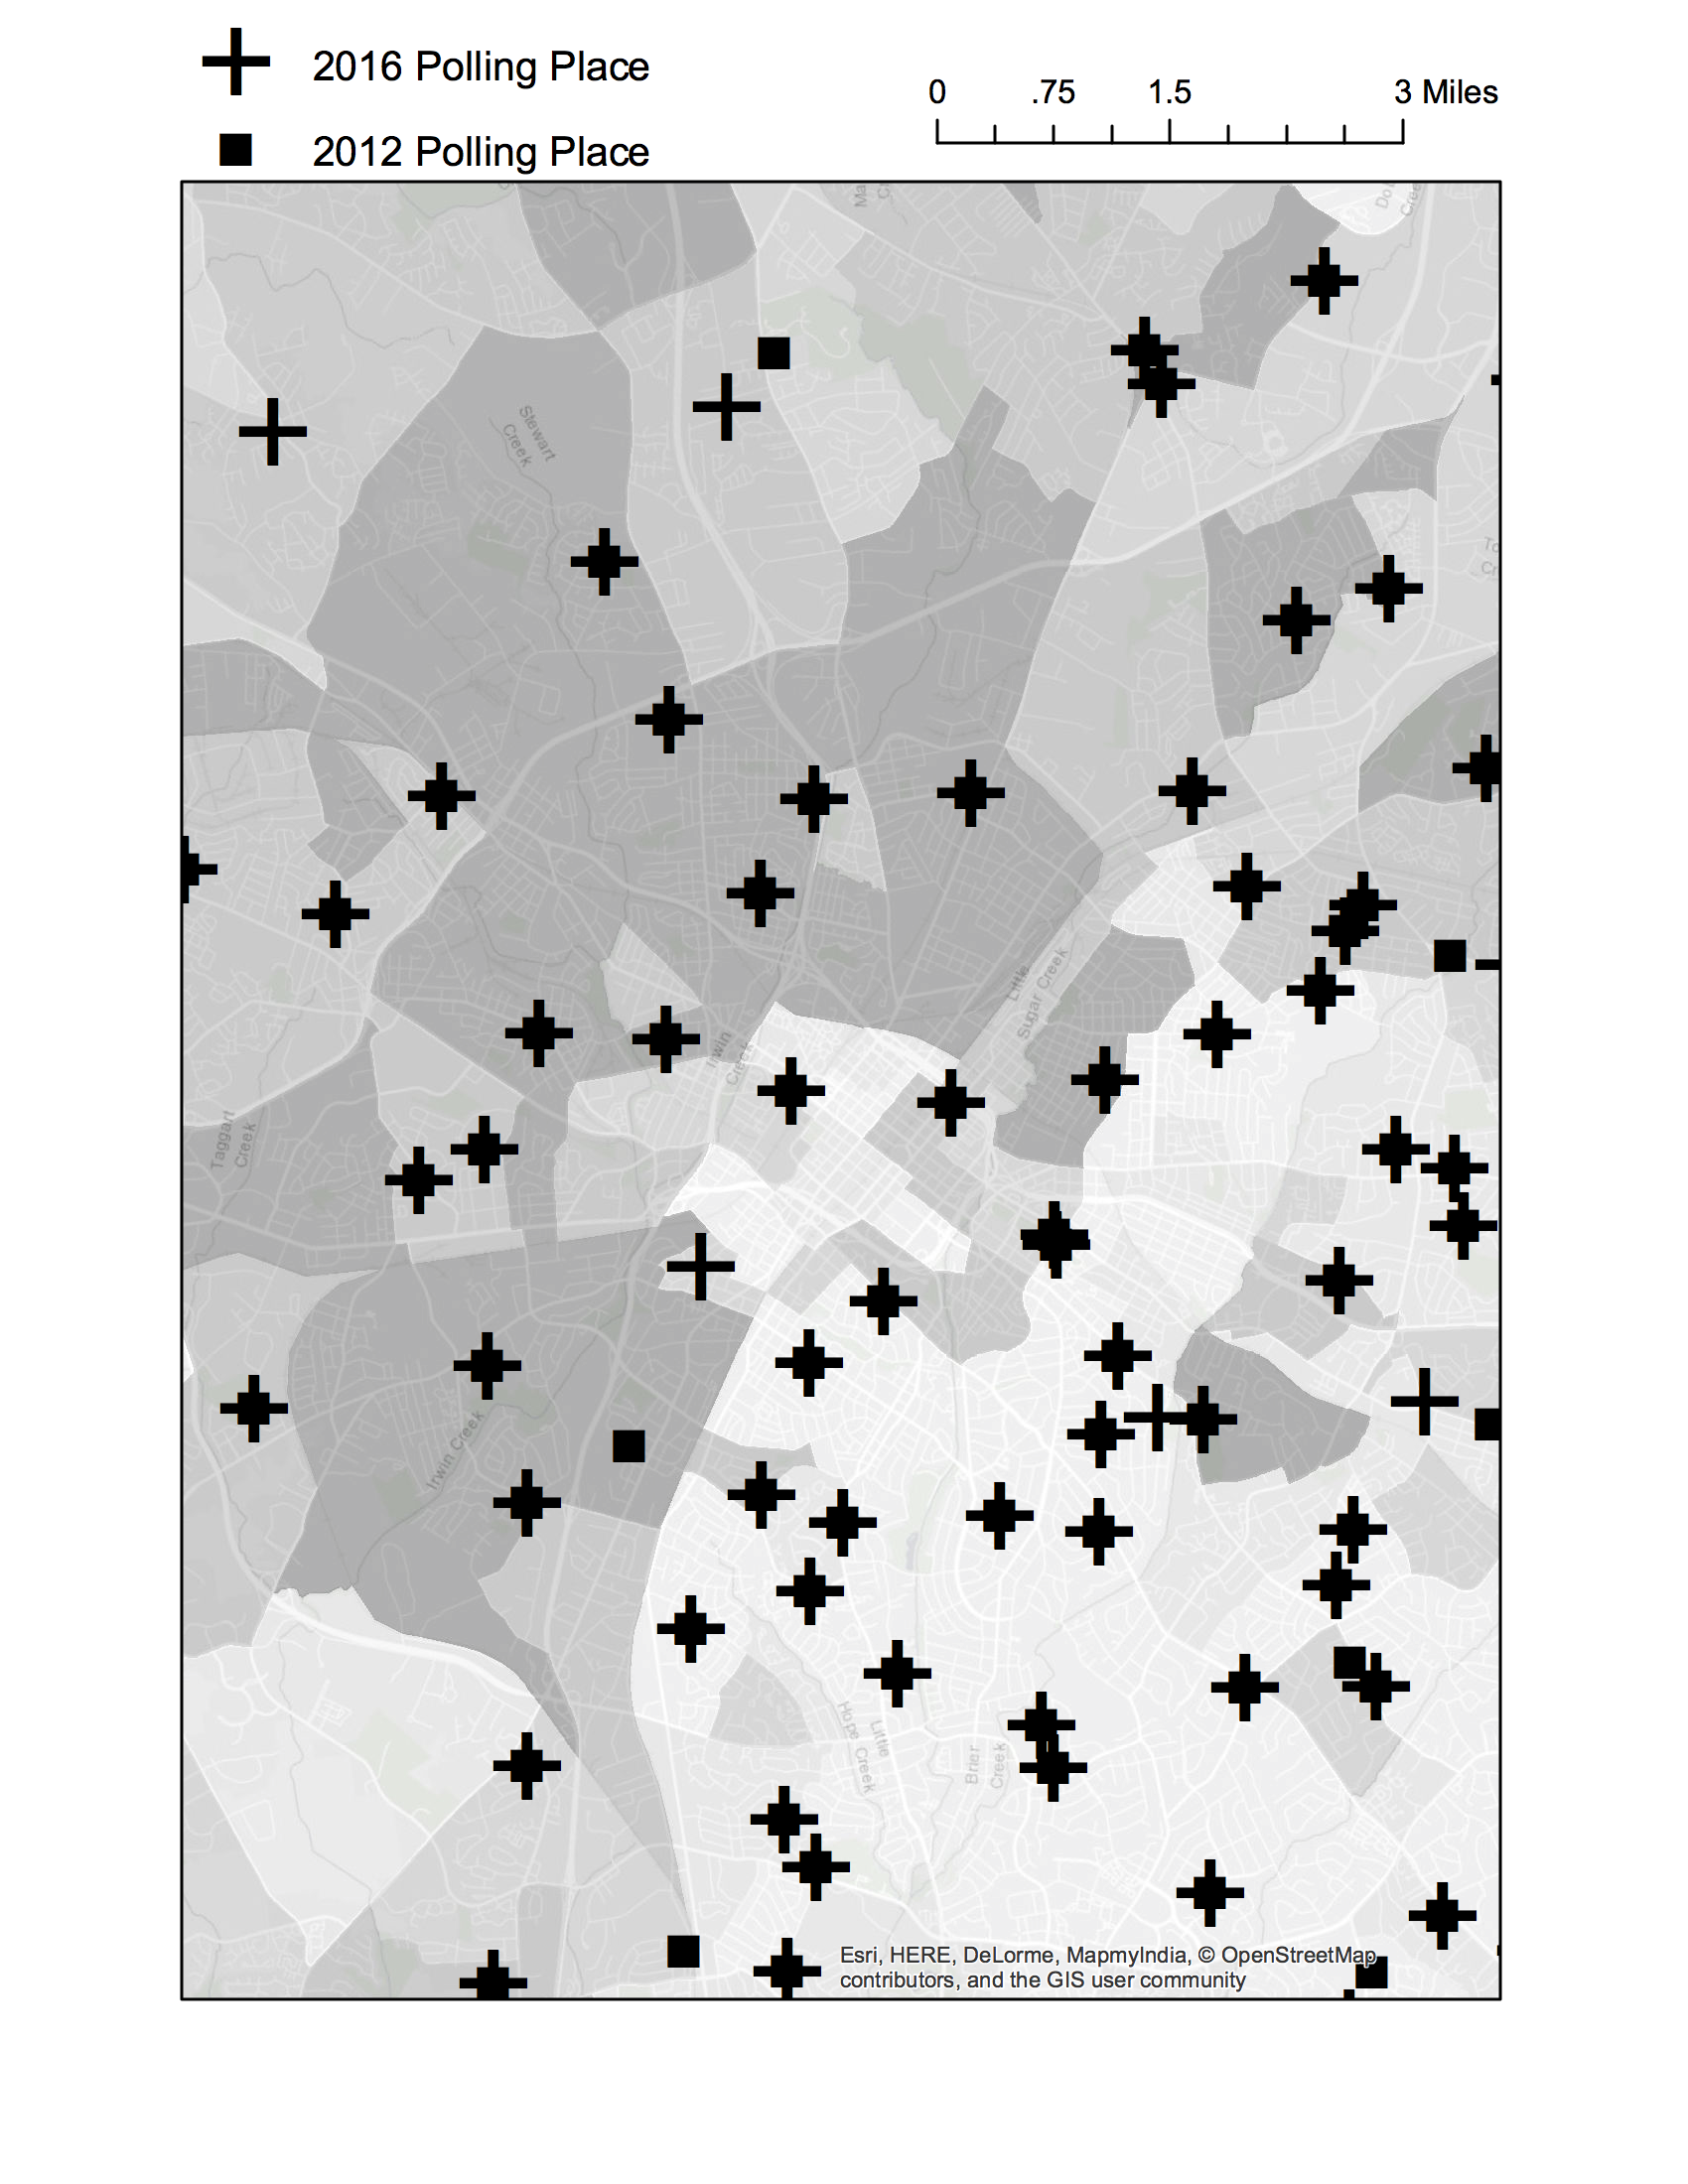
\includegraphics[ width=1.3in,  clip=true,  trim= 1.0in 10.13in 4.9in 0.5in ]{../../50_results_full/Map_Charlotte_PP_Legend_A.png}
				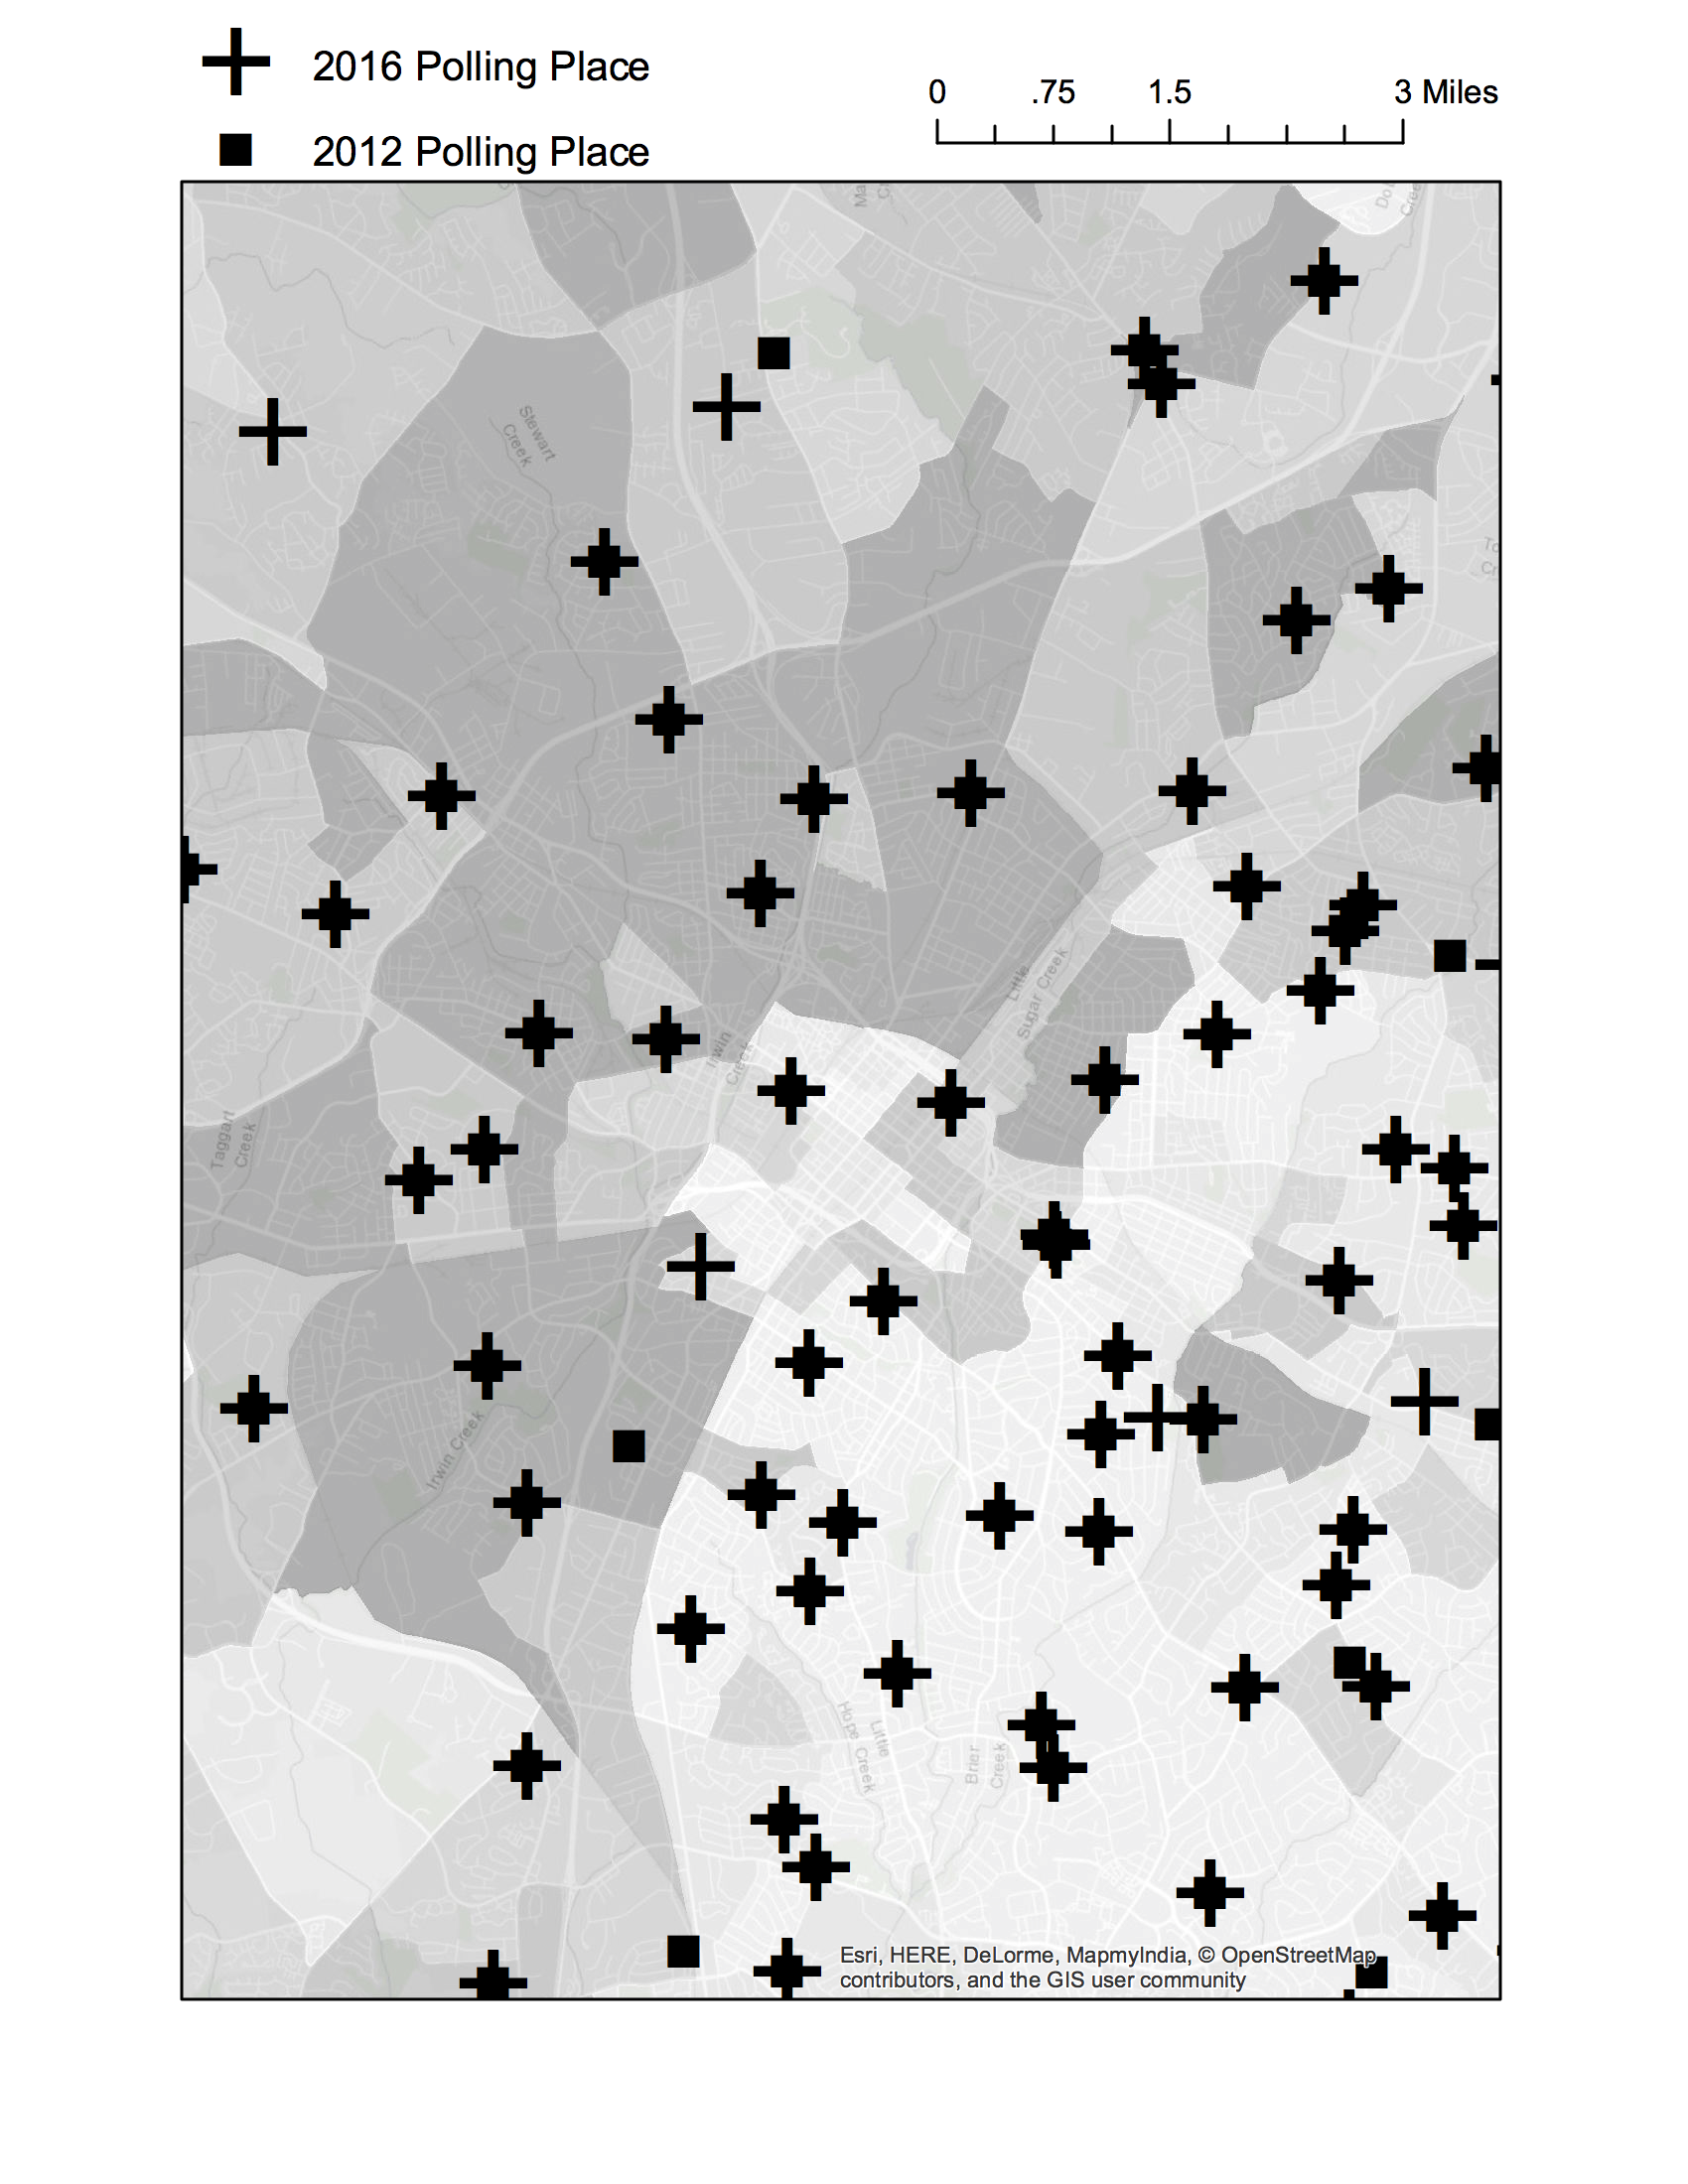
\includegraphics[ width=1.3in,  clip=true,  trim= 1.0in 10.55in 4.9in 0in ]{../../50_results_full/Map_Charlotte_PP_Legend_A.png}
		\vspace*{.05in}
		\label{figure_map_charlotte_pp}
		\end{center}
	\scriptsize{\emph{Notes:}   The above maps illustrate movement in polling place locations using the example of central Charlotte in Mecklenburg county.  Map (a) presents the locations of polling places in 2008 (Xs) and 2012 (squares). Map (b) presents the locations of polling places in 2012 (squares) and 2016 (crosses).  The background is shaded according to the racial composition of census block groups in the 2010 census with darker shades of gray indicating a higher percentage of black residents.  Gray boundaries indicate 2016 precinct boundaries with precinct \#22's boundary outlined in bold black.}
\end{figure} \normalsize

In addition to identifying whether a voter's polling place has changed between presidential elections, we are also able to measure how far voters have to travel from their residence to reach their polling place.  We use Google Directions API to estimate how long it takes every voter to reach their polling place by car in minutes from the population-weighted centroid of their Census block at 10am on Election Day, Tuesday, November 6th, 2018.\footnote{Estimating travel times for census block centroids rather than for each voter's residence is necessary for financial and computational reasons.  However, Census blocks are \emph{extremely} small units --- they are less than an acre, typically between 0.7 and 0.9 of an acre.  This minimizes though of course does not eliminate measurement error.  This is highly likely to be classical measurement error that attenuates our travel time results rather than biasing them.  When we present our results we note the small substantive magnitude of our effects (not only the statistical significance).   We use a future date because Google only provides travel time estimates for future dates.}  Using estimated travel times is important because straight-line distance measures may mask substantial variation in actual travel times depending on road density and traffic congestion.\footnote{Even so, a limitation of using travel times by car is that it may still mask substantial variation in travel times using public transportation, as well as travel time that reflects where people work or run typical errands (and thus what their usual travel route is).  As poor and minority voters are more likely to use public transportation to reach their polling place, we attempt to account for these differences by looking at heterogeneity in the effects of travel costs by race and income. As for our inability to account for where people work, unless there is a systematic difference in where polling places are re-located relative to workplaces, this should attenuate but not bias our results.}

Figure \ref{figure_traveltime_distribution} plots the distribution of polling place changes in terms of the proximity between the old and new polling places (Plot (a)) and the change in predicted drive times between old and new polling place (Plot (b)).  Most polling places experienced relatively small changes in their location --- unsurprising, given the size of precincts and the availability of suitable alternative sites --- and travel times did not systematically increase or decrease.  In general, conditional on experiencing a polling place, very few voters had their travel times changed by more than 5 minutes --- indeed 5 and a half minutes represents two standard deviations of the distribution.  Other work has measured distance rather than travel time in the context of polling place changes \citep{brady2011turning,haspel2005location}, nevertheless, the average treatment in existing work (between a half of a mile to a mile) is of a similar magnitude to what we document in terms of travel time.  Thus, for the vast majority of voters we study, the treatment dosage is comparable to existing work.\footnote{The differences arise primarily because where previous studies have looked at Los Angeles and Atlanta, we study both urban and rural areas.  Thus our distribution has much longer tails.  In the analysis, we analyze effects for those who experience ``small'' versus ``large'' changes to their drive time, which effectively allows us to estimate differential effects for urban versus rural voters.}


%% FIGURE: Distribution of distance pp moved, and drive time to pp
%%---------------------------------------------------------------------------------------
\begin{figure}[t!]
	\begin{center}
	\caption{Distribution of Distance of Polling Place Changes and Changes in Drive Time}
		\small \vspace*{.05in}
		\bigskip
		\hspace*{.4in} (a) Change in Distance Between Past   \hspace*{0.8in} (b) Change in Drive Time to Polling Place \\
		  and Current Polling Place Location  \hspace{2.75in} \text{ } \\
		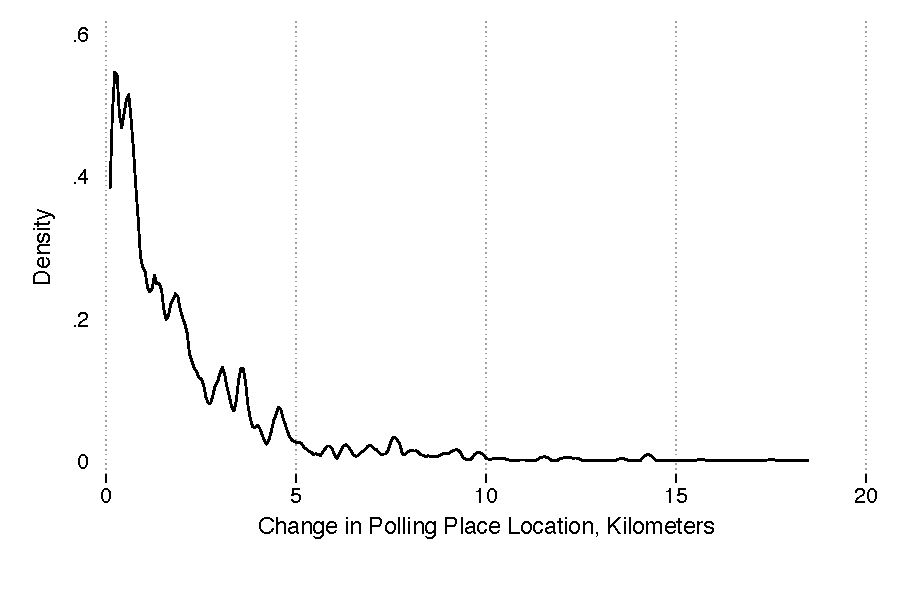
\includegraphics[ width=3in,  clip=true,  trim= 0.0in 0in 0in 0in ]{../../50_results_full/Plot_Distribution_PPMoveDistance.pdf}
		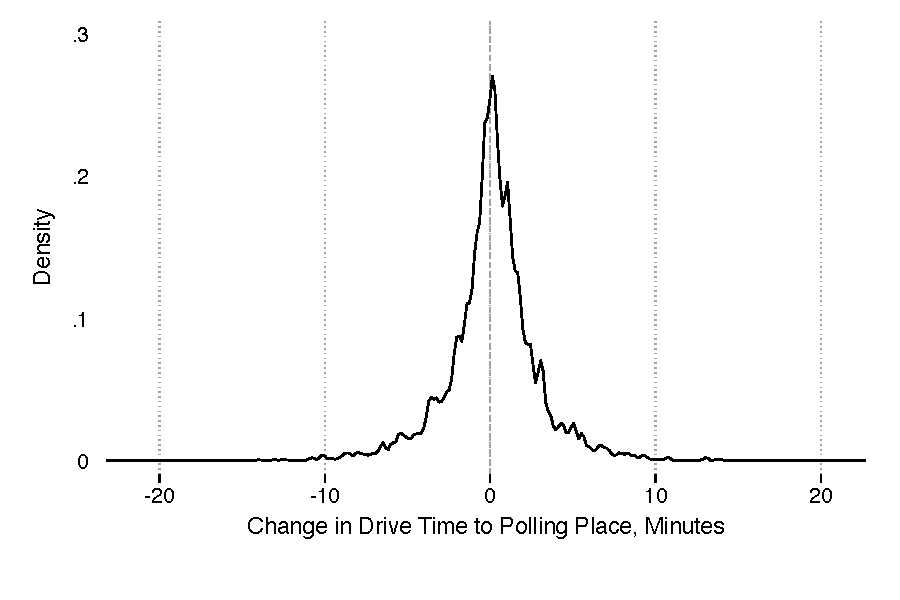
\includegraphics[ width=3in,  clip=true,  trim= 0.0in 0in 0in 0in ]{../../50_results_full/Plot_Distribution_DriveTime.pdf}
		\label{figure_traveltime_distribution}
		\end{center}
	\scriptsize{\emph{Notes:}  Plot (a) presents the distribution of the distance between a precinct's polling place location in a given election year relative to its location in the previous election year, conditional on a voters' polling place having moved. The data is pooled across 2012 and 2016. The unit of analysis in plot (a) is a voter-election; therefore, distance changes are weighted by the number of voters experiencing the change in a given year.  Polling place changes can result from the movement of a given individual's polling place, or from a voter being moved into a new precinct by a precinct boundary change.  Plot (b) presents the distribution of changes in drive time to a polling place for voters who experienced a polling place change.  Note that some voters can experience a polling place change without a change in drive time.    There are not qualitative differences in the distribution of changes for either of the measures between the two years.  We present the separate years in Appendix H.}
\end{figure} \normalsize

While the question of why polling places are moved is a fascinating one, work by \cite{clintontargering2018} shows that the partisanship and race of a voter is uncorrelated with the probability that the voter experiences a change in polling place location. While we do not think that polling places are moved randomly, the lack of a relationship demonstrated in  \cite{clintontargering2018} suggests that officials are not obviously moving polling places in a way explicitly designed to affect turnout by targeting certain types of voters,  thus negating a potentially large confounder in our analysis.




%------------------------------------- ESTIMATION: TURNOUT --------------------------------------------%
\section{The Effect of Polling Place Changes on Turnout}\label{section_empirical_main}

\noindent We begin by considering the average effect of polling place location changes on overall turnout.  We include controls for travel costs to differentiate between the impact of a change \emph{per se} --- which theory predicts should depress turnout either through search costs, confusion or habit disruption --- and the impact of changes in the costs of voting caused by changes in travel times to the polls. We examine the effects for overall turnout, as well as the effect on Election Day and early turnout, specifically, since changes to the cost of Election Day voting may affect whether voters choose to vote early, in addition to whether they turnout at all.

Figure \ref{figure_bar_pp_change} descriptively plots how polling place changes correspond with voter turnout for the 2012 and 2016 presidential elections.  Plot (a) shows that voters who experience a change in their polling place location are less likely to vote on Election Day --- a decline that occurs regardless of whether the changes occur in 2012 or 2016.  However, Plot (b) shows that early voting \emph{increased} among affected voters such that the overall relationship with turnout (Plot (c)) is effectively null.  On average, the aggregate difference between Election Day and early voting appears to be negligible.  This is surprising given our strong theoretical priors on the negative costs associated with moving polling places.


%  FIGURE: Bar plot of polling place changes and voting by year
%-------------------------------------------------------------
\begin{figure}[t!]
	\begin{center}
	\caption{Descriptive Relationship Between Polling Place Changes and Turnout Type by Year}
		\small \vspace*{.05in}
		\smallskip
		  (a) Election Day Voting  \hspace*{0.9in} (b) Early Voting \hspace*{1.1in} (c) All Voting  \\
				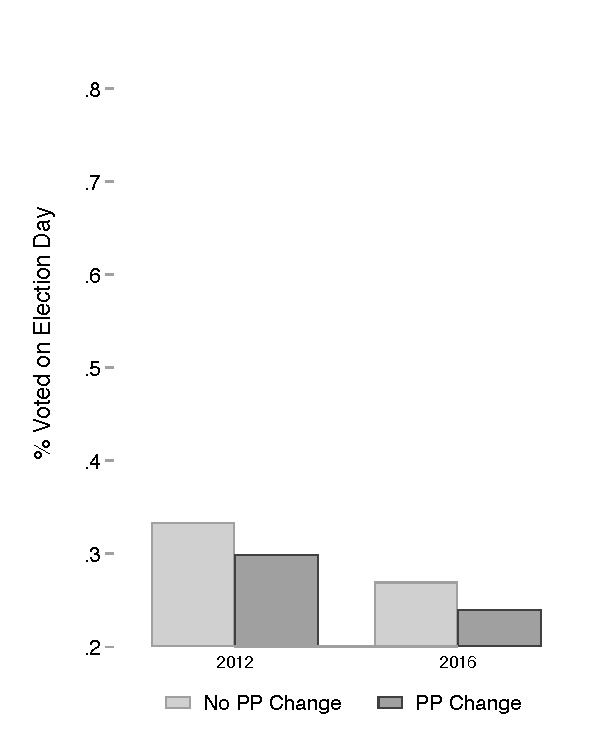
\includegraphics[ width=2in,  clip=true,  trim= 0.0in 0.4in 0in 0in ]{../../50_results_full/Plot_Bar_Vote_elecday.pdf}
				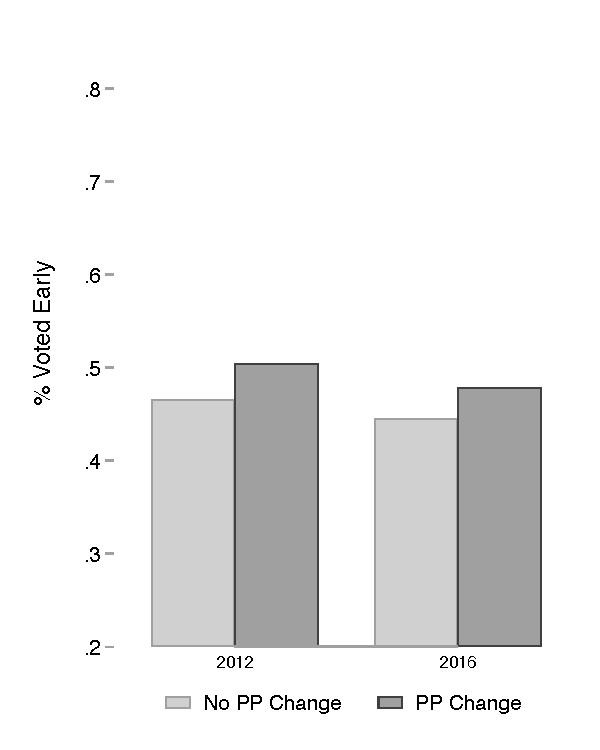
\includegraphics[ width=2in,  clip=true,  trim= 0.0in 0.4in 0in 0in ]{../../50_results_full/Plot_Bar_Vote_early.pdf}
				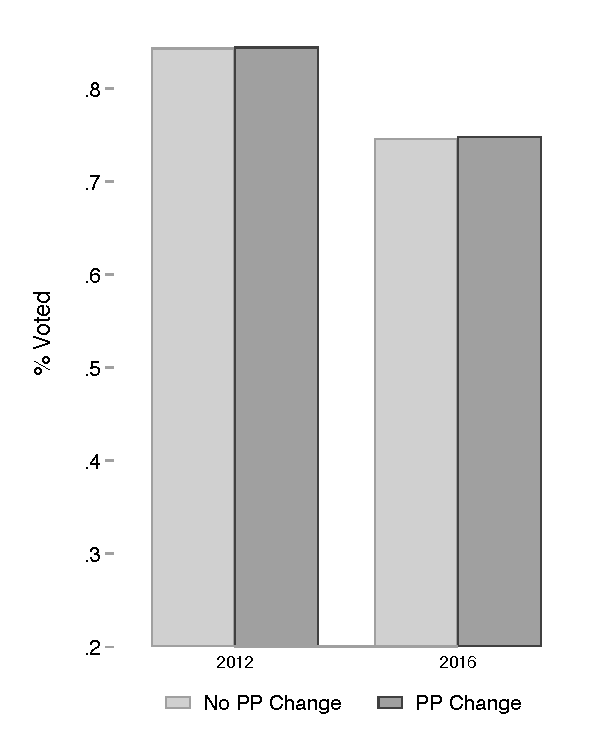
\includegraphics[ width=2in,  clip=true,  trim= 0.0in 0.4in 0in 0in ]{../../50_results_full/Plot_Bar_Vote_any.pdf} \\
				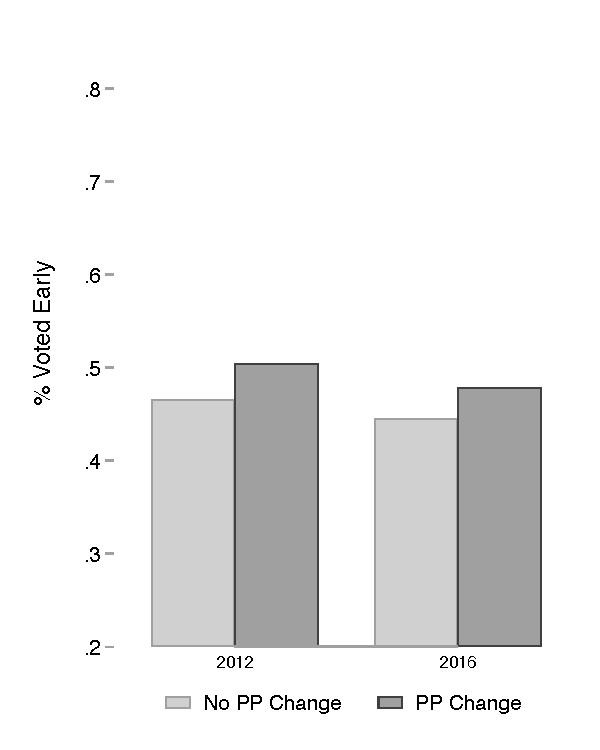
\includegraphics[ width=2.5in,  clip=true,  trim= 0.0in 0.0in 0in 4.5in ]{../../50_results_full/Plot_Bar_Vote_early.pdf}
		\label{figure_bar_pp_change}
		\end{center}
	\scriptsize{\emph{Notes:}  The bar plots present mean voter turnout by year by whether an individual experienced a polling place change relative to the previous presidential election year.  Plot (a) presents the relationship for Election Day voting only, plot (b) presents the relationship for early voting, and plot (c) presents the relationship for all types of voting (total turnout).  The residual category is absentee voting which represents a minuscule proportion of voting in North Carolina.  Note that the y-axes are the same for each plot, but do not include zero to better visualize differences between categories and years.}
\end{figure} \normalsize


To visualize how these relationships depend on travel time, Figure \ref{figure_scatter_drivetime} plots the change in estimated drive time in minutes to the current year's polling place relative to the previous polling place for each Election Day voting (Plot (a)) and early voting (Plot (b)).  The hollow circles denote the binned average turnout by voting mode for every 2 minute interval of drive time change.  The descriptive plots show only a small relationship between travel costs and voting, except at the extreme tails of travel time changes.  This is perhaps due to the small size of most North Carolina precincts. The tails in Figure \ref{figure_scatter_drivetime} indicate a lower likelihood of Election Day voting (and a higher likelihood of early voting) for those moved further from their polling place, while the reverse is true for those moved closer.  This suggests that the decision to vote early in response may be conditioned by how close or far a polling place is moved.


%  FIGURE: Scatterplots of drive time
%------------------------------------
\begin{figure}[t!]
	\begin{center}
	\caption{Descriptive Relationship Between the Change in Driving Time to Polling Place and Type of Voting}
		\small \vspace*{.05in}
		\smallskip
		\hspace*{.1in} (a) Election Day Voting  \hspace*{1.8in} (b) Early Voting \\
				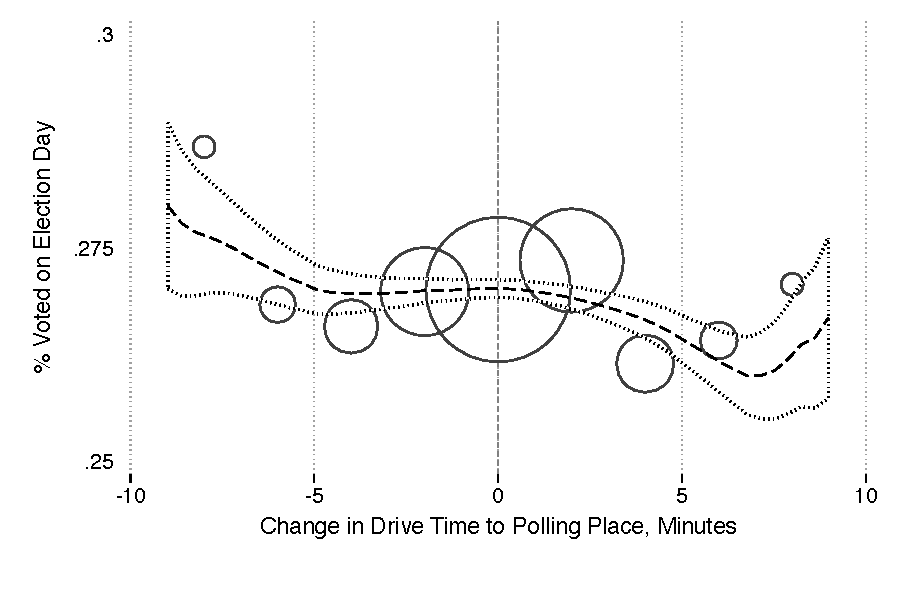
\includegraphics[ width=3in,  clip=true,  trim= 0.0in 0in 0in 0in ]{../../50_results_full/Plot_Scatter_DriveTime_elecday.pdf}
				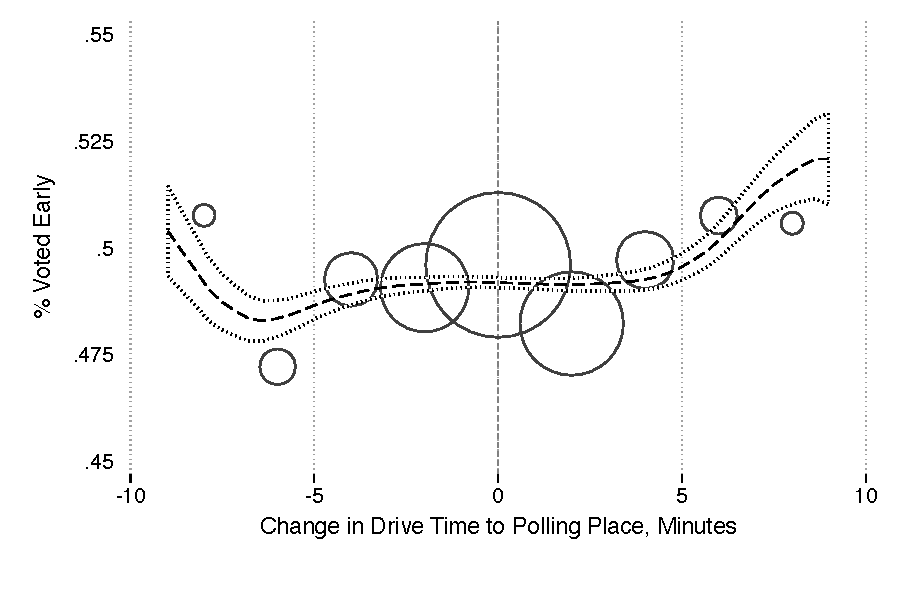
\includegraphics[ width=3in,  clip=true,  trim= 0.0in 0in 0in 0in ]{../../50_results_full/Plot_Scatter_DriveTime_early.pdf}
		\label{figure_scatter_drivetime}
		\end{center}
	\scriptsize{\emph{Notes:}   The plots graph the change in drive time to polling place in minutes (closer,<0, or further, >0) from the previous presidential election year and the percentage of individuals voting early (Plot (a)), and on Election Day (Plot (b)). Plots are conditional on voters experiencing a polling place change in either 2012 or 2016.  Hollow circles are binned averages of the outcome for every 2 minute interval of drive time change and they are sized relative to the population in the bin (excluding changes in drive times that are greater than the 99th percentile of drive time changes).  The dashed line represents a local polynomial fit (bandwidth = 3) to all data for changes that within the 99th percentile.  We exclude data not in the 99th percentile while at the same time not fitting a linear relationship because the sensitivity of linear fits to extreme outliers.  Note that the y-axis are different.}
\end{figure} \normalsize


These descriptive plots suggest minimal overall turnout effects as a consequence of polling place changes, in addition to only minimal turnout effects as a consequence of \emph{where} polling places are moved relative to voters. To better identify the impact of polling place changes on turnout beyond these descriptive results requires controlling for factors associated with an individual's likelihood of voting and estimating the counterfactual of how those same voters would have behaved in the absence of a polling place change.  Existing work seeks to identify the effect of polling place changes by matching voters based on observables \citep{brady2011turning} or statistically controlling for observables \citep{amos2017reprecincting} to compare the behavior of voters who are and are \emph{not} impacted by a polling place change.  Comparing the turnout behavior of individuals who share observable demographic features is certainly reasonable, but it may produce misleading estimates if the groups differ in terms of unmeasured or unmeasur\emph{able} characteristics.\footnote{Although matching is certainly a defensible alternative strategy and can reduce some parametric assumptions required for this fixed effects strategy, we consider the ability to control for \emph{all} time-invariant individual characteristics and specific time-varying unobserved confounders, as our strategy does, preferable to matching on observables.  }  % Given the individual-level co-variates that we have access to, the only non-fixed feature of voters is their turnout in the ``pre-treatment'' period: 2008.

We weaken the identification assumptions required by \emph{between}-individual comparisons and estimate the counterfactual by leveraging our balanced panel to provide a \emph{within}-individual comparison that is better able to account for all of the ways that individuals may differ in their propensity to vote, and to vote by a given mode.  Thus, we track how polling place changes affect the behavior of the same voters over time, controlling for fixed \emph{individual}-level differences that may affect the likelihood and method of voting.\footnote{We do \emph{not} contend that  the inclusion of individual fixed effects means that voters will never change voting modes for their own reasons, as other work documents \citep{stein1997}; rather, the fixed effects allow us to say that there is no difference in the \emph{likelihood of changing modes across people with and without polling place changes}.}  These fixed individual-level differences \emph{also} control for stable-over-time differences in voting that may be caused by, or associated with, differences in neighborhood, precinct, or county.  Therefore, our within-individual identification of the effect of polling place changes results from comparing how the turnout of an individual experiencing a polling place change varies relative to the turnout behavior of the \emph{same} individual when they do not experience a polling place change.\footnote{To be clear, voters who always vote or never vote are included in our sample and contribute meaningful variation to our estimates.  The only voters who are not included in our estimation as a consequence of our use of voter fixed effects are voters who \emph{always or never} experience a polling place change.  For those voters, it is not possible to determine how those individuals would have behaved in the absence of (or the presence of) of a polling place change.}

Because we are also concerned that there may be time-varying factors that affect both the movement of polling places and the turnout behavior of voters, we leverage our large sample size to estimate a set of fixed effects interactions to account as best as possible for such confounders.  Insofar as we think individuals of different races may have different trends in turnout and choice of mode of voting, we control for differential generalized trends in turnout by race.  We are also able to control for differential trends by the fixed characteristics of counties that might impact \emph{both} when and where polling places are moved \emph{and} how voters cast their ballots  (e.g. changes in the availability of county-level early voting).  Together, these strategies help to alleviate concerns about time-varying omitted variable bias; in other words, bolstering the (inherently un-testable) parallel trends assumption. Results for our 2012 cross-section where we are able to estimate the relationship between future polling place changes and contemporaneous turnout (after accounting for past polling place changes and other covariates) further support a causal interpretation for the majority of our results -- that is that past turnout behavior does not predict future polling place changes in a way that would bias our results.\footnote{Appendix N presents these results. They indicate no relationship between future polling place changes and neither early voting nor turnout in general.  There may be a negative relationship between future polling place changes and contemporaneous Election Day turnout, but if anything, this suggests that the negative Election Day turnout results that we find are \emph{over}estimating the true causal effect, consistent with our overall story.  It's also important to note that, while helpful, these lead regressions are not our preferred specifications since they cannot include our full set of fixed effects and fixed effect interactions. } Finally, we might be concerned that polling place location changes are being conducted in a targeted and partisan manner (as work such as \cite{amos2017reprecincting} argue occurs).  However, as previously noted, research by \cite{clintontargering2018} finds no evidence that polling place changes in North Carolina  are correlated with voters' party registration or race -- suggesting that the data generating process for polling place changes is not strategically designed to influence turnout.

More formally, for voter $i$, in county $c$, during presidential election year $t$, we estimate the average effect of polling place changes on turnout using the following OLS specification:\footnote{We use OLS to estimate a linear probability model (LPM) rather than a logit or probit model to increase interpretability, improve computation, and avoid the incidental parameters problem arising with the use of fixed effects in non-linear models such an a multinomial probit or logit.}
\begin{align}
	Pr(Vote_{i,t}) = \boldsymbol{\alpha_{i}} + \boldsymbol{\gamma_{t}}  + \beta \Delta PollingPlace_{i,t}
    +\delta \Delta MuchFurther_{i,t}  \label{equation_traveltime_panel} \\
    + \lambda \Delta MuchCloser_{i,t} + \boldsymbol{\mu}(\boldsymbol{Race_{i}} \cdot \boldsymbol{Year_{t}}) + \boldsymbol{\tau}(\boldsymbol{County_{c}} \cdot \boldsymbol{Year_{t}})  + \epsilon_{i,t} \nonumber
\end{align}


\noindent where $Pr(Vote_{i,t})$ is an indicator for whether a vote is cast, $\Delta PollingPlace_{i,t}$ is an indicator equal to $1$ if voters experienced a change in the location of their polling place from the previous presidential election year, $\Delta MuchFurther_{i,t}$ is an indicator equal to 1 if a voter's polling place was moved more than 5 minutes drive time further from them, and $\Delta MuchCloser_{i,t}$ is an indicator equal to 1 if a voter's polling place was moved more than 5 minutes closer to them (the residual category contains voters whose polling place is moved less than 5 minutes closer \emph{or} further; that is, voters with a small change in drive time, either positive or negative). Conditional on a polling place change, a 5 minute change in travel time is approximately equal to two standard deviations of the travel time variation.  Thus, this measurement strategy allows us to effectively compare ``standard changes'' to extreme changes in a straightforwardly interpretable way.\footnote{The conditional standard deviation is     2.8\unskip.  Theoretical guidance on the expected functional form of the relationship between travel time and turnout is limited.  Thus our dichotomization at two standard deviations is both a data-driven choice reflecting how the relationship looks in Figure~\ref{figure_scatter_drivetime}, as well as choice to ease interpretability of our results (particularly when we add additional interactions).  Because this approach imposes somewhat restrictive parametric assumptions, Appendix E reports substantively identical results using alternative specifications of travel time.  One could also think of ``standard'' versus ``extreme'' changes as reflecting changes made in urban versus rural settings.}  Note that because we are comparing presidential elections, every voter in every precinct has the same top-of-the-ticket race in each election. $\boldsymbol{Race_{i}}$ is a vector of race indicators which we interact with year indicators to account for differential turnout trends over time amongst different races, $\boldsymbol{County_{c}}$ is a vector of county indicators, which we interact with year indicators ($\boldsymbol{Year_{t}}$) to account for differential turnout trends by county that may result from population changes or early voting changes, $\boldsymbol{\alpha_{i}}$ are individual fixed effects that capture level differences in the probability of voting for each individual in our sample, and $\boldsymbol{\gamma_{t}}$ are year fixed effects that account for common shocks to individuals by year.   Although we have data on past voting behavior, but we do not included lagged dependent variables as doing so introduces Nickell bias \citep{Nickell:1981eo} in panels with individual fixed effects when the N dimension of the panel is substantially larger than the T dimension. Finally, $\epsilon_{i,t}$ is the idiosyncratic error term.  We (robustly) cluster our standard errors by shared precinct assignment histories to account for serial correlation and the hetereoskedasticity of errors in a linear probability model.\footnote{Precincts are not stable over time, therefore we use the group formed by a common history of precinct assignments (whether a non-moving voter was ever part of the same precinct as another non-moving voter in our sample) as our clustering unit.  This is slightly more conservative than clustering on one set of precincts in one time period.}

The coefficient $\beta$ estimates the \emph{general} marginal impact of a polling place change, while $\delta$ and $\lambda$ are the \emph{additional} impacts of a significant decrease ($\delta$) or increase ($\lambda$) in travel time.  Of primary interest is the relative impact of a change of any kind ($\beta$) --- costs that represent the net impact of search costs, confusion, habit disruption and any priming effects --- versus travel costs ($\delta$,$\lambda$).  Because the average marginal effect of a polling place change regardless of travel time is also an important quantity of interest, we also estimate equation~\ref{equation_traveltime_panel} without the travel time indicators (i.e. excluding $MuchFurther$ and $MuchCloser$).  This effect constitutes the population-weighted average impact of a polling place change.





% TABLE 4: Average Effect of Polling Place Changes and Drive Time Changes
%------------------------------------------------------------------------

\begin{table}[t!]\centering \footnotesize
\def\sym#1{\ifmmode^{#1}\else\(^{#1}\)\fi}
	\caption{The Average Effect of Polling Place Changes and Drive Time on Voter Turnout}\label{table_pp_panel}
	\smallskip
	\begin{tabular}{@{\extracolsep{5pt}}l*{6}{c}}
	\noalign{\smallskip}\hline\hline\noalign{\smallskip}\noalign{\smallskip}
			&  \multicolumn{2}{c}{$Pr(VoteElecDay)$} &  \multicolumn{2}{c}{$Pr(VoteEarly)$} &  \multicolumn{2}{c}{$Pr(VoteAny)$}  \\
			\cline{2-3} \cline{4-5} \cline{6-7} \noalign{\smallskip}
				                &\multicolumn{1}{c}{(1)}         &\multicolumn{1}{c}{(2)}         &\multicolumn{1}{c}{(3)}         &\multicolumn{1}{c}{(4)}         &\multicolumn{1}{c}{(5)}         &\multicolumn{1}{c}{(6)}         \\
\midrule
$\Delta$\emph{PollingPlace} $(\hat{\beta})$&  -0.0073\sym{**} &  -0.0067\sym{*}  &   0.0063\sym{*}  &   0.0058         &  -0.0015         &  -0.0015         \\
                & (0.0037)         & (0.0037)         & (0.0037)         & (0.0038)         & (0.0015)         & (0.0016)         \\
$\Delta$\emph{MuchCloser} $(\hat{\lambda})$&                  &    0.014         &                  &   -0.011         &                  &   0.0022         \\
                &                  &  (0.012)         &                  &  (0.013)         &                  & (0.0059)         \\
$\Delta$\emph{MuchFurther} $(\hat{\delta})$&                  &   -0.031\sym{**} &                  &    0.027\sym{*}  &                  &  -0.0026         \\
                &                  &  (0.014)         &                  &  (0.014)         &                  & (0.0054)         \\
\midrule
Individual FE   &\checkmark         &\checkmark         &\checkmark         &\checkmark         &\checkmark         &\checkmark         \\
Year FE         &\checkmark         &\checkmark         &\checkmark         &\checkmark         &\checkmark         &\checkmark         \\
County x Year FE&\checkmark         &\checkmark         &\checkmark         &\checkmark         &\checkmark         &\checkmark         \\
Race x Year FE  &\checkmark         &\checkmark         &\checkmark         &\checkmark         &\checkmark         &\checkmark         \\
Year Sample     &Full Panel         &Full Panel         &Full Panel         &Full Panel         &Full Panel         &Full Panel         \\
Observations    &  4681792         &  4681792         &  4681792         &  4681792         &  4681792         &  4681792         \\
Mean of DV      &     0.30         &     0.30         &     0.46         &     0.46         &     0.80         &     0.80         \\
SD of DV        &     0.25         &     0.25         &     0.26         &     0.26         &     0.21         &     0.21         \\
 \\  %% CHANGE THIS
	\noalign{\vspace*{-.17in}}\hline\hline\noalign{\smallskip}
\multicolumn{7}{p{6.1in}}{\scriptsize Standard errors clustered by precinct assignment history. } \\
\multicolumn{7}{l}{\scriptsize \sym{*} \(p<0.1\), \sym{**} \(p<0.05\), \sym{***} \(p<0.01\)}\\
\multicolumn{7}{p{6.1in}}{\scriptsize  \emph{Notes}: The table presents coefficients from estimating Equation~\ref{equation_traveltime_panel} with and without the travel time indicators.  The unit of analysis is the voter-election.  See Table \ref{table_pp_panel_combined_wcontrols} in Appendix C for the full set of coefficient estimates.  The SD of the DV is the average of the within-$i$ standard deviations of the outcome variable. $Pr(VoteAny)$ includes non-in-person modes of voting, like mail-in voting, and thus the mean of the $VoteElecDay$ and $VoteEarly$ do not sum to the mean of $VoteAny$.  The residual category for $MuchCloser$ and $MuchFurther$ are voters whose polling place is moved less than 5 minutes drive \emph{either} closer or further.  ``Full panel'' refers to panel regressions estimated on our balanced panel of voters, as opposed to cross-sectional regressions estimated on voters from that panel.}
\end{tabular}
\end{table}


Existing work suggests that voters may respond to increased costs to one method of voting by switching their mode of voting \citep{michelson2012effect}.  Therefore, we not only estimate the effect of \emph{whether} a voter voted, but also \emph{how} they cast their ballot.  To do so, we estimate Equation~\ref{equation_traveltime_panel} separately for the following outcomes: whether the voter voted on Election Day ($Pr(VoteElecDay)$), whether the voter voted early ($Pr(VoteEarly)$), and whether they voted \emph{at all} regardless of method ($Pr(VoteAny)$).

Our results are presented in Table~\ref{table_pp_panel}.  We find that polling place changes decrease Election Day turnout for our balanced sample of non-movers. Indeed the average effect is to reduce Election Day turnout by    -0.7\unskip~percentage points (column 1).  In addition, this is due in part to the polling place change \emph{per se}, and in part due to changes in travel costs --- being moved further from one's polling place depresses Election Day turnout by approximately    -3.1\unskip~percentage points \emph{more} than a voter who experiences a drive time change of less than 5 minutes --- but the effects are not symmetric.  Polling places that are moved significantly closer increase Election Day turnout, but by a much smaller amount ($\hat{\lambda}$).\footnote{In Appendix E, we allow the slope as well as the intercept to differ for polling places moved 5 minutes closer/further.  We find that there is a more negative slope for those whose drive time is made longer by more than 5 minutes in terms of their Election Day turnout, and a more positive slope for early voting.  Thus, they substitute statistically significantly more.  However, the magnitude of the difference in substitution is small.}  The finding that polling place changes decrease Election Day voting --- especially for polling place changes that are moved more than 5 minutes away --- is consistent with prior findings, albeit for a longer panel, and larger sample of voters across an entire state.

Table~\ref{table_pp_panel} also reveals a more novel and striking finding --- the negative effects of a polling place chance on Election Day voting are nearly entirely offset by substitution into early voting. On average, polling place changes increase early voting by     0.6\unskip~percentage points (column 3). Moreover, voters who are moved much further from their polling place are     2.7\unskip~percentage points \emph{more} likely to vote early relative to those who remain relatively close by, but voters are no more or less likely to vote early if their polling place is moved much closer.  Columns 5 and 6 confirm that these effects are nearly completely offsetting --- the decrease in Election Day voting and the increase in early voting combine to produce less than a half-percentage point point overall change in turnout.

Overall, the results suggest that polling place changes do not decrease overall turnout --- even those that greatly increase travel costs --- but they do lead voters to change how they vote.\footnote{As noted previously, we find a differential decline in turnout for those voters who move residences in such a manner that they would have voted at their same polling place had the location not been administratively moved.  The magnitude of this differential decline is 1 percentage point.  See Appendix O. }  At least in the high-stakes presidential election contests we examine, voters respond to an increase in the costs of voting on Election Day by casting their vote early. Moreover, although all voters are more likely to vote early in response to a polling place change, the substitution effects are nearly three times larger for voters whose polling places are moved more than 5 minutes further away from their residence. Because most polling place changes result in travel time changes of less than 5 minutes, however, it is the disruptive impact of a change \emph{per se} that is most responsible for changes in voter behavior (as evidenced by the similar magnitudes of the estimates of $\hat{\beta}$ in Table~\ref{table_pp_panel}).

One explanation for these results is \emph{substitution} between modes of voting --- voters who \emph{would have} voted on Election Day, instead decided to vote early when their polling place was changed.  However, it is alternately possible that polling place changes induce a population of non-voters to vote early --- potentially by the mailers informing them of a polling place change and priming them to turnout --- and a distinct (but coincidentally equal sized) population of Election Day voters failed to vote on election day. As discussed in detail in Appendix G, additional analyses suggest that our results are primarily driven by substitution --- the increase in early voting occurs among those who otherwise would have voted on Election Day absent the polling place change. As the counter-factual intention of voters is unobservable, however, these results can only be suggestive.





%% ---------------------------------- SECTION: COUNTY HETEROGENEITY ---------------------------------- %%
\section{Effects of Polling Place Changes by County}\label{section_countylevel}

\noindent In this section we investigate the extent to which the average state-wide effects we estimate in the previous section hide county-level heterogeneity.  To be clear, because we leverage within-voter variation, the average statewide effects we identify are crucially not a function of county-level differences in the propensity to vote, or vote by a particular mode.  Even so, characterizing the county-level variation in the effects of polling place changes is important for situating our statewide estimates vis-a-vis the results of prior studies based on changes in a single locality.  Insofar as there is considerable between-county variation in the effects of polling place changes occurring within the same state and election, it is difficult to generalize such ``local'' estimates.  The difficulty of generalizing impacts not only our ability, as a discipline, to identify the mechanisms of impact, but also the ability to predict how the effects of polling place changes might affect election outcomes by affecting turnout.

To estimate the county-level effects of polling place changes on turnout, we use the equation~\ref{equation_traveltime_panel} to separately estimate the effects of a polling place changes for the subset of our voter-level panel residing in each county.\footnote{The estimation excludes the county-by-year fixed effects as these are un-estimable at the county level.  Standard errors continue to be clustered by precinct assignment history.}  To summarize the results, Figure~\ref{county_elec_appendix} plots the county-specific coefficient estimates ($\hat{\beta}$) that identify the effect of a polling place change on Election Day voting. Bars around each estimate show the naive 95\% confidence interval, while estimates in red marked with solid diamonds are also statistically significant after a multi-test correction to keep the False Discovery Rate below 5\% using a \cite{Benjamini:2006gd} two-step multi-test correction. (The appendix reports the estimated effects for early voting (Figure~\ref{county_early_appendix}).)  Our null hypothesis remains $H_{0}: \hat{\beta}=0$ because our interest in is whether the analysis of any given individual county could provide evidence that polling place changes decrease (or even increase) turnout or result in statistically significant substitution between voting modes, \emph{not} whether counties differ from the average effect we calculated before (to which any given county contributed variation).


%% FIGURE: County plots of the effect of polling place change on early voting turnout
%%-----------------------------------------------------------------------------------
\begin{figure}[t!]
	\begin{center}
	\caption{County-Specific Estimates of the Effect of a Polling Place Change on Election Day Voting}
		\small \vspace*{.05in}
		\smallskip
		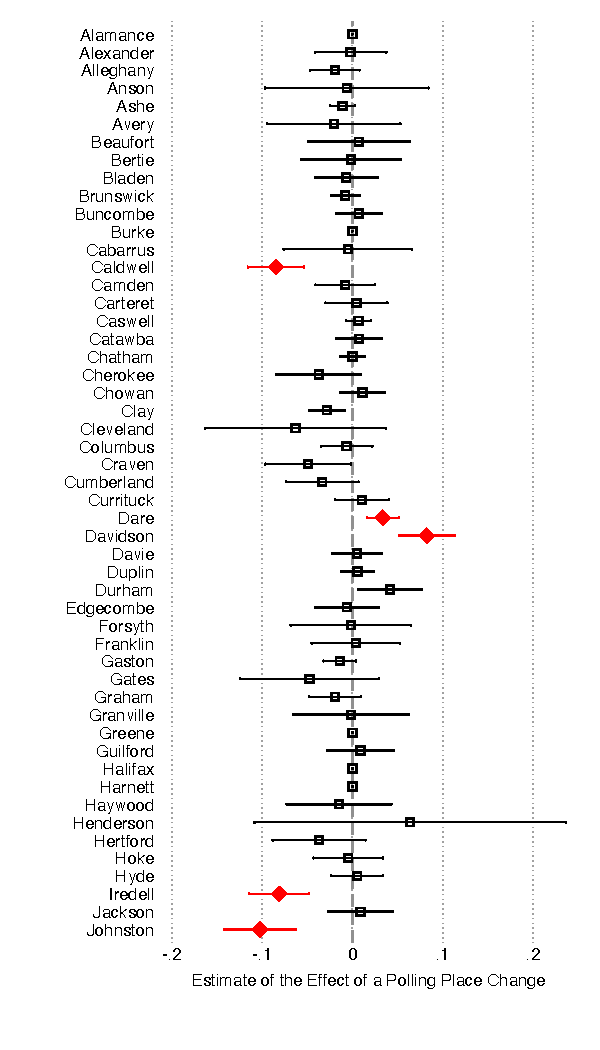
\includegraphics[ width=3in,  clip=true,  trim= 0.0in 0in 0in 0in ]{../../50_results_full/Plot_County_Coefficients_elecvote1.pdf}
		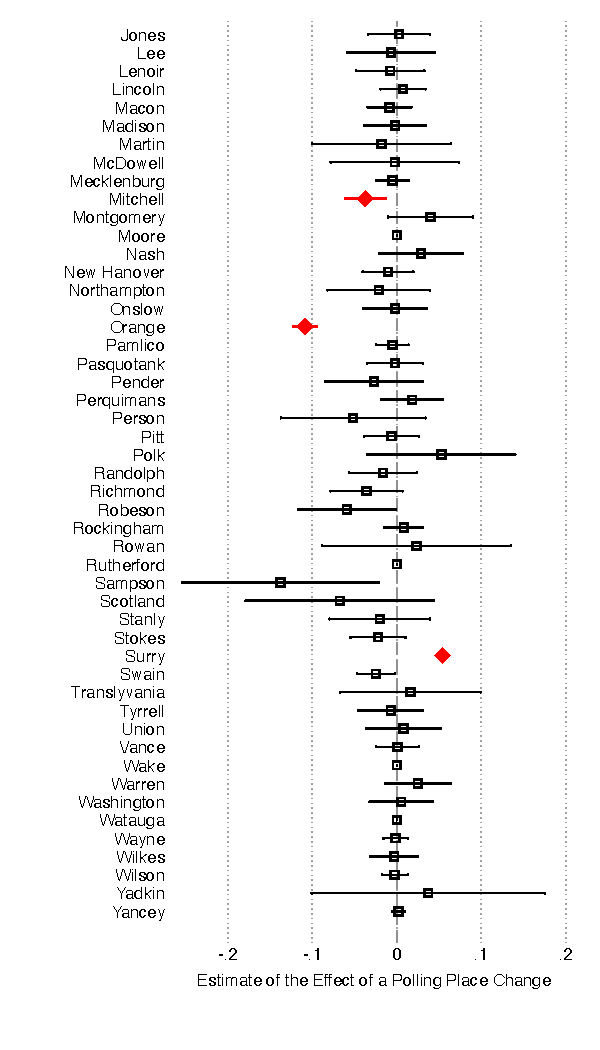
\includegraphics[ width=3in,  clip=true,  trim= 0.0in 0in 0in 0in ]{../../50_results_full/Plot_County_Coefficients_elecvote2.pdf}
		\label{county_elec}
		\end{center}
	\scriptsize{\emph{Notes:}The above plot presents estimates of Equation~\ref{equation_traveltime_panel} for each county individually along with 95\% confidence intervals.  The outcome is $Pr(VoteElecDay)$.  Estimates are plotted with naive 95\% confidence intervals clustered by precinct assignment history. Red estimates whose point estimates are plotted as solid diamonds are statistically significant after applying the \citet{Benjamini:2006gd} multiple test correction with a False Discovery Rate limit of 0.05; insignificant estimates are black squares.  Some county estimates cannot be estimated because no precincts in those counties experienced a polling place change. }
\end{figure} \normalsize

Figure~\ref{county_elec} reveals substantial heterogeneity in the estimated effect of a polling place change between counties when using the conventional levels of statistical significance that would be employed when studying the effects in an individual county. In fact, we recover estimates of the effect of a polling place change on Election Day voting that vary in direction, magnitude and statistical significance.  For example, polling place changes in Sampson county were estimated to decrease the probability of a voter casting an Election Day vote by nearly 15\%, but the changes made in Polk county were estimated to increase the probability of voting on Election Day by nearly 5\%.  Insofar as data limitations have forced existing work to estimate the impact of polling place changes using limited geographies, the variation we document highlights the difficulty of generalizing to the state-wide level from a specific, or set of specific, localities.

Figure~\ref{county_any} plots the county-level coefficient estimate ($\hat{\beta}$) of the effect of a polling place change on overall turnout regardless of method (i.e. the net effect of Election Day and early voting).  (For space, we include the early voting figures in Appendix F).  The figure shows that after employing multi-test corrections to account for the fact that we are essentially performing multiple hypothesis tests, we find only four counties where effects on turnout are statistically different from zero (two with positive effects and two with negative effects). In contrast, the results in ten additional counties would suggest that there are statistically significant effects on turnout if we relied on conventional (naive) p-values when analyzing individual counties --- including Richmond, one of most populous counties in North Carolina. As a consequence, were the findings of a selected single county generalized, one could potentially conclude that polling place changes have a radical impact on turnout whereas a more systematic analysis does not.


%% FIGURE: County plots of the effect of polling place change on overall turnout
%%-------------------------------------------------------------------------------------------------------
\begin{figure}[t!]
	\begin{center}
	\caption{County-Specific Estimates of the Effect of a Polling Place Change on Overall Voter Turnout}
		\small \vspace*{.05in}
		\smallskip
		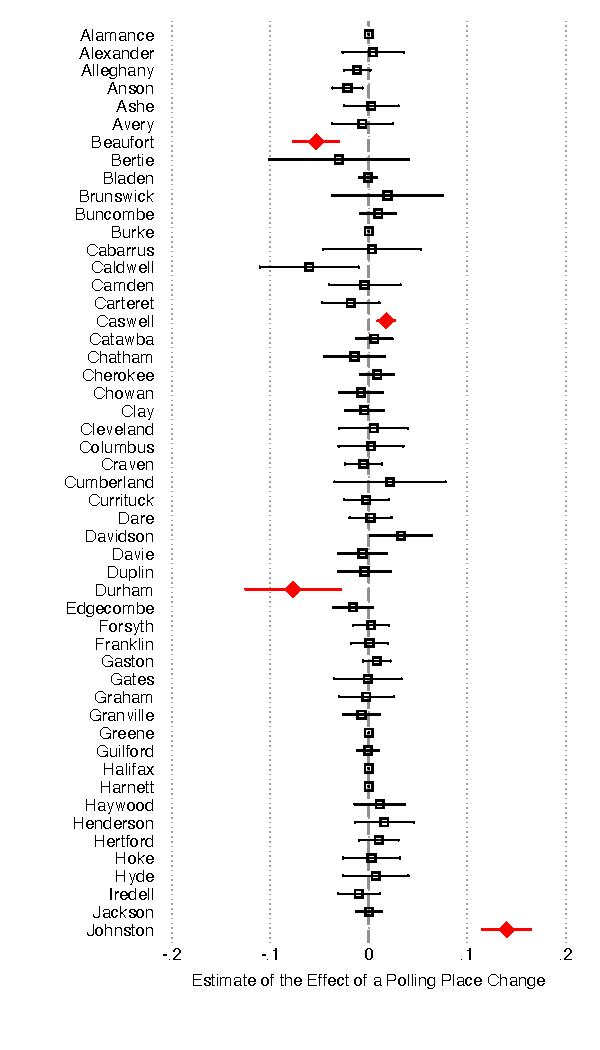
\includegraphics[ width=3in,  clip=true,  trim= 0.0in 0in 0in 0in ]{../../50_results_full/Plot_County_Coefficients_anyvote1.pdf}
		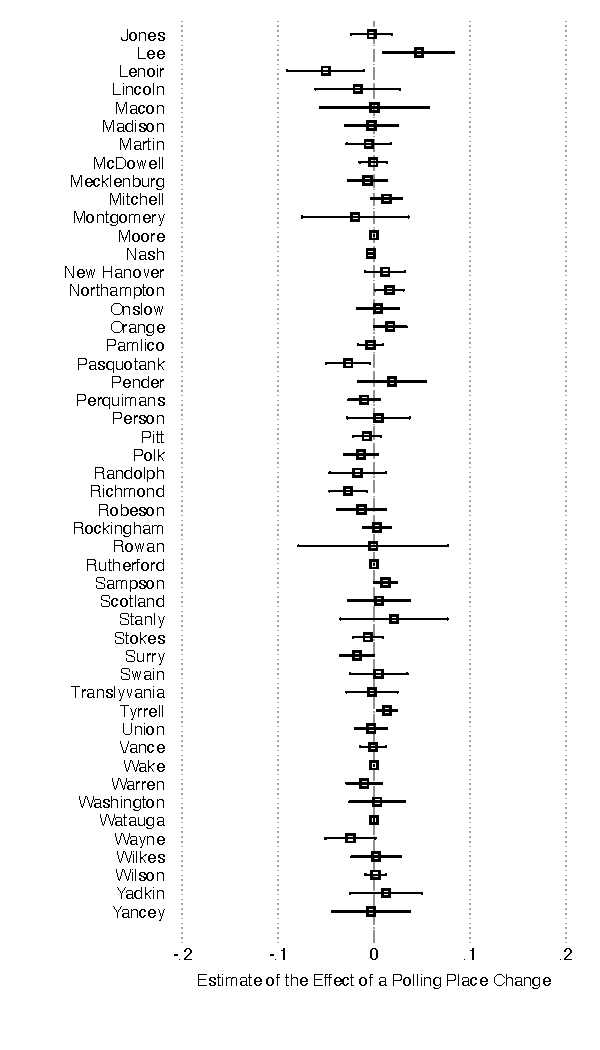
\includegraphics[ width=3in,  clip=true,  trim= 0.0in 0in 0in 0in ]{../../50_results_full/Plot_County_Coefficients_anyvote2.pdf}
		\label{county_any}
		\end{center}
	\scriptsize{\emph{Notes:}  The above plot presents estimates of Equation~\ref{equation_traveltime_panel} for each county individually along with 95\% confidence intervals.  The outcome is $Pr(VoteAny)$.  Estimates are plotted with naive 95\% confidence intervals clustered by precinct assignment history. Red estimates whose point estimates are plotted as solid diamonds are statistically significant after applying the \citet{Benjamini:2006gd} multiple test correction with a False Discovery Rate limit of 0.05; insignificant estimates are black hollow squares.  Some county estimates cannot be estimated because no precincts in those counties experienced a polling place change. }
\end{figure} \normalsize

One possibility is that perhaps the county-level differences reflect differential effects caused by compositional differences in the counties being compared --- e.g., the availability of early voting in the county, the percentage of lower-resourced voters in the county who are less able to overcome the costs imposed by a polling place change.\footnote{We note again that other work on North Carolina finds no evidence that partisan election administrators differentially target voters of different parties or races in a way that suggestions an intent to manipulate turnout \citep{clintontargering2018}.}  To consider whether this is the case, we now examine whether the average substitution effect varies in the ability to vote early or according to voter characteristics that may impact the ability or willingness to overcome the costs of a polling place change.






%%---------------------------- SECTION: Heterogenous Effects ----------------------------------- %%
\section{Differential Effects of Polling Place Changes by Early Voting Availability and Race}\label{section_heterogeneity}

\noindent Our results show that, on average, polling place changes create a substitution effect from Election Day voting to early voting.  We now probe this relationship in more detail to determine whether the substitution effects we identify vary depending on characteristics that are plausibly related to voters' ability to overcome the costs created by polling place changes. We focus in the text on two characteristics: (1) the availability of early voting, and thus the ease of substituting to early voting; and (2) the race of affected voters, which might be related to the resources that voters have to overcome costs associated with polling place changes and/or the desire of voters that have been historically disenfranchised to overcome increased costs of voting. Additional analyses in Appendix I and Appendix K examine whether the effects vary by age and income, respectively.\footnote{In the case of differential effects by age, we find evidence that middle aged voters are more likely to substitute relative to \emph{both} older and younger voters, but no differences in the overall turnout effect of polling place changes by age.  In the case of differential effects by income, we find differences in rates of substitution --- with wealthier voters less likely to substitute into early voting --- but no overall turnout effects.}

%% Subsection: Early voting
%%------------------------
\subsection{Differential Impacts by the Availability of Early Voting}

All North Carolina counties had at least one early voting site in each of the presidential elections that we study.  However, the number of those sites, and the hours that those sites were open differed between counties and over time.  Although the stability of the location of early voting sites is also of interest, the fact that there is not a one-to-one mapping of voters to early voting locations, and the fact that voters can use any early voting location in a county makes it more challenging to construct a simple voter-level indicator for change.    The average effects we identify in Section~\ref{section_empirical_main}  control for these differences using voter-level fixed effects and interactions between county fixed effects and year indicators, but we might expect that variation in early voting availability would moderate the effect of polling place changes and the magnitude of the substitution effects we identify.  Increased access to early voting might increase the likelihood of substituting into early voting, although there is disagreement in the literature about how beneficial early voting is \citep{burden2017complicated,burden2014election,herron2015race,fullmer2015}.\footnote{The availability of other forms of ``convenience voting" have also been associated with mixed turnout results \citep{gronke2007early, karp2000going, kousser2007does, gerber2013identifying}.}

To evaluate whether the effects of polling place changes depend on the availability of  early voting,  we estimate a cross-sectional version of our panel specification (equation~\ref{equation_traveltime_panel}) without the travel time indicators.  We do this separately for each county and the outcome $Pr(VoteEarly)$.  We then compare the resulting coefficients on the impact of a polling place change ($\hat{\beta}$) with measures of early voting availability (results demonstrating the same relationship for population-normalized early voting are in Appendix J).  Figure~\ref{figure_scatter_earlyvotingavailability} summarizes the relationship reported in Appendix F between the county-level effects of a polling place change ($\hat{\beta}$) and the number of early voting locations in a county (Plot (a)) and the total number of hours that early voting is available in a county (Plot (b)).\footnote{This data was obtained from the county boards of election for both 2012 and 2016 from \url{https://dl.ncsbe.gov/?prefix=One-Stop_Early_Voting/2016/}.}

Again highlighting the difficulty of generalizing from specific localities when assessing the effects of polling place changes on turnout and outcomes, Figure~\ref{figure_scatter_earlyvotingavailability} reveals tremendous variation not only in the availability of early voting across counties, but also in the estimated effects of a polling place change on the likelihood of voting early (as Figure~\ref{county_elec_appendix} documents). (Appendix J plots the distributions of early voting availability by partisan election administration regime.)\footnote{We by no means deny that our statewide effects average across potentially very different effects in different counties.  Exploring the county-level variation in the estimated effects is important (and is one of the reasons that we document such variation the previous section of the paper).  But the focus of our paper is on the overall impact of polling place changes at the state level, rather than theorizing and testing the reasons \emph{why} the effects may vary across counties.}  Because we are interested in the average statewide effect of polling place changes, we use the county-level estimates to examine whether the county-level substitution effects vary depending on the relative availability of early voting in the county.

%  FIGURE: Scatterplots for Early Voting
%----------------------------------------------------
\begin{figure}[t!]
	\begin{center}
	\caption{Relationship Between Early Voting Availability and Early Voting by Year}
		\small \vspace*{.05in}
		\bigskip
		\hspace*{.4in} (a) Number of Early Voting Locations  \hspace*{1.0in} (b) Hours of Early Voting Availability \\
				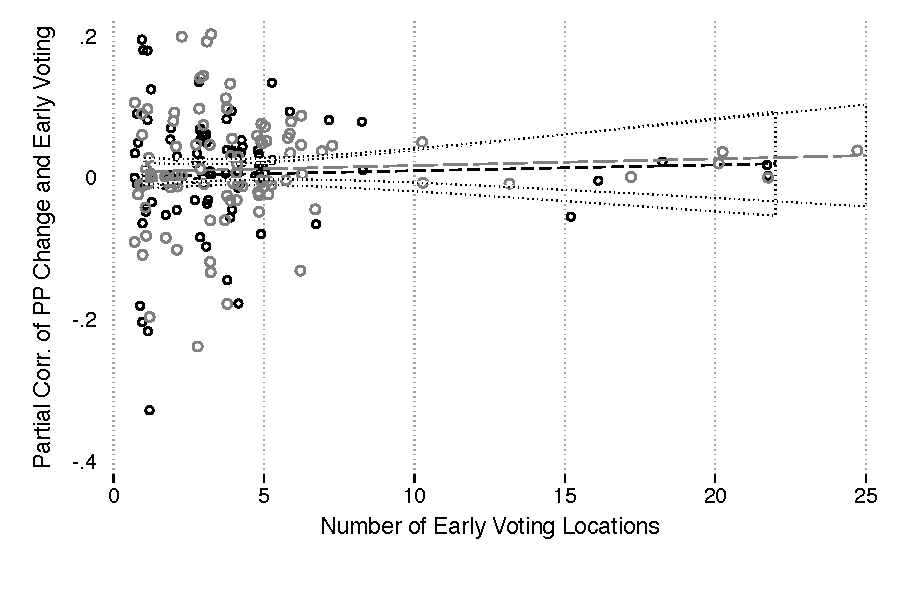
\includegraphics[ width=3in,  clip=true,  trim= 0.0in 0in 0in 0in ]{../../50_results_full/Plot_Scatter_EarlyLocations_EarlyVote.pdf}
				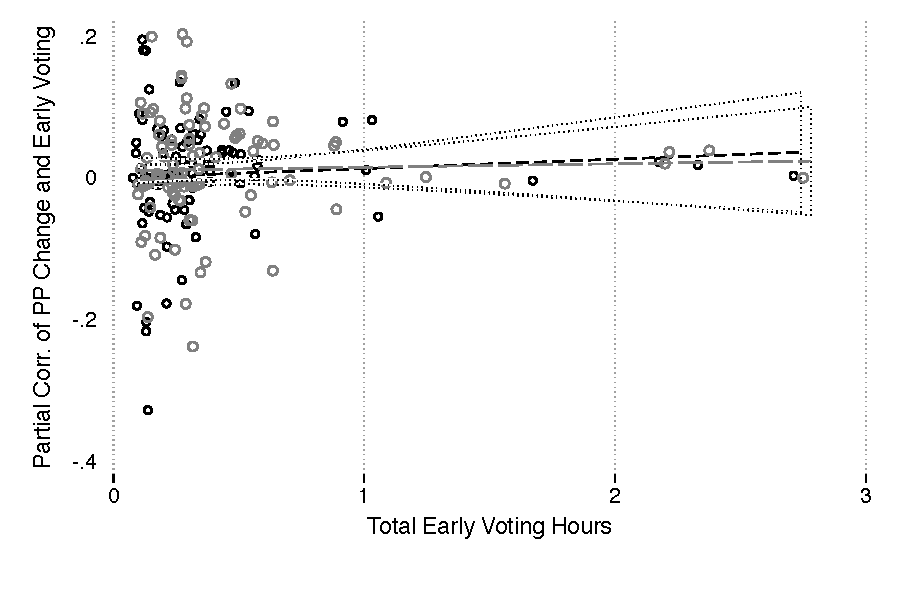
\includegraphics[ width=3in,  clip=true,  trim= 0.0in 0in 0in 0in ]{../../50_results_full/Plot_Scatter_EarlyHours_EarlyVote.pdf} \\ \vspace*{-.12in}
				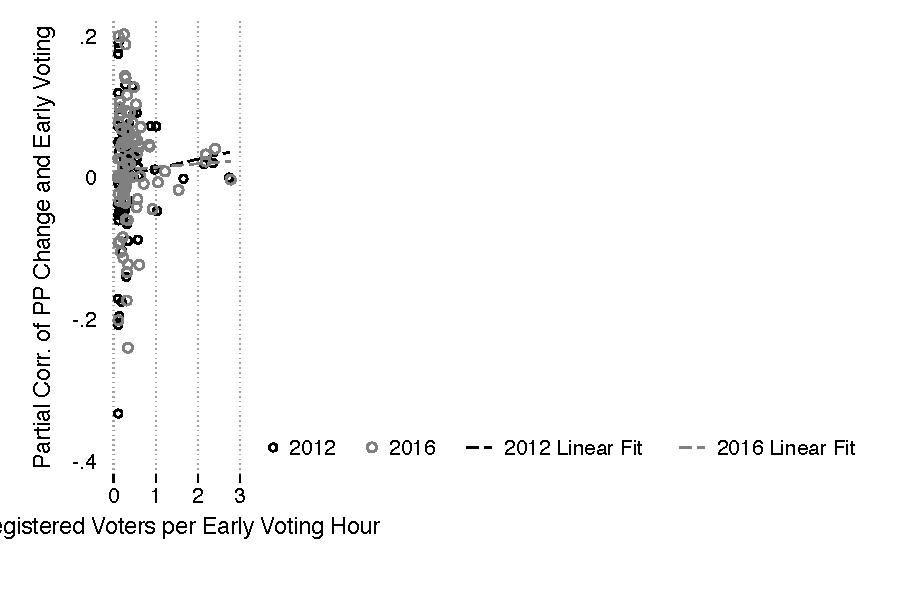
\includegraphics[ width=4.0in,  clip=true,  trim= 0.5in .2in 0in 3.3in ]{../../50_results_full/Plot_Scatter_EarlyHours_Legend.pdf}
		\label{figure_scatter_earlyvotingavailability}
		\end{center}
	\scriptsize{\emph{Notes:}   Plot (a) represents the relationship between the number of early voting locations and the average effect of a polling place change on early voting by county.  Plot (b) represents the relationship between the total number of early voting hours (in thousands) and the average effect of a polling place change on early voting by county.  The average effect of a polling place on early voting by county is obtained by estimating Equation~\ref{equation_traveltime_panel} as a cross-section separately for each county using the outcome of $Pr(VoteEarly)$.  Points are jittered to aid visualization and linear fits are plotted with 95\% confidence intervals.  Identical relationships that normalize early voting availability by county population are found in Appendix J and exhibit the same lack of systematic relationship.}
\end{figure} \normalsize

The plotted regression lines reveal that the variation in the county-level substitution effects we estimate do not correlate meaningfully with early voting availability in either 2012 or 2016 --- a result borne out  by formal regression estimates and investigations that disaggregate early voting hours by weekends and evenings.  The results are also qualitatively the same as estimates that normalize all measures of early voting availability by county population to ensure that variation in the characteristics of differently populated counties do not account for the lack of correlation (Appendix J). With the qualification that our analysis of early voting does not account for early voting location movement (a fruitful avenue for future research), our results suggest that other mechanisms other than the availability of early voting must be responsible for the substitution effects that we identify.


%% Subsection: Race
%%------------------
\subsection{Differential Impacts by Race}\label{subsection_racehetero}

The history of race and disenfranchisement in North Carolina is long and fraught.  That recent battles over election administration have frequently centered on race-based voter suppression suggests that which voters of which race vote is of critical contemporary importance in the state \citep{insightus2016, vasilogambros2018, michaelson2016, roth2015, berman2016}. In this section we explore potential differences in our effects by race.  Doing so helps us to understand some aspects of the historical legacy of voter disenfranchisement, as well as speaking to the ability of different voters to overcome the costs associated with polling place changes.

Our expectations regarding the differential effects of polling place changes by race are ambiguous. On the one hand, the effects of polling place changes may be larger, on average, among black voters because of differences in material resources that allow voters to overcome costs \citep{verba1995voice, wolfinger1980votes, leighley2013votes}, or the availability of early voting by race \citep{fullmer2015race}. However, the effect of limited resources may be mitigated by greater value placed on voting by groups with a past history of struggling to secure voting rights \citep{anollnorms} or by other social norms that tend to incentivize turnout in high salience elections \citep{doherty2017voting}.  Race-related mobilization efforts such as ``souls to the polls'' events may also differentially moderate the effect of polling place changes.

To investigate whether polling place changes have larger or smaller effects depending on the race of the affected voters, we estimate our panel with the addition of an interaction between polling place change and an indicator for non-white voters --- classifying a voter as non-white if they ever indicate that they are such in the voter rolls.  We collapse racial categories into a binary ``white'' and ``non-white'' (including hispanics) category to aid interpretability, but similar effects are obtained by estimating separate effects by disaggregated race (Appendix D).  Blacks by far constitute the largest group of non-whites in North Carolina and our racially disaggregated results in the appendix suggest our effect is primarily a function of the voting behavior of blacks.


% TABLE 6: Polling Place Changes by Mode of Voting,Race
%----------------------------------------------------------------------------
\begin{table}[t!]\centering \footnotesize
\def\sym#1{\ifmmode^{#1}\else\(^{#1}\)\fi}
	\caption{The Differential Effects of Polling Place Changes by Race}\label{table_pp_nwhite}
	\smallskip
	\begin{tabular}{@{\extracolsep{5pt}}l*{6}{c}}
	\noalign{\smallskip}\hline\hline\noalign{\smallskip}\noalign{\smallskip}
			&  \multicolumn{2}{c}{$Pr(VoteElecDay)$} &  \multicolumn{2}{c}{$Pr(VoteEarly)$} &  \multicolumn{2}{c}{$Pr(VoteAny)$}  \\
			\cline{2-3} \cline{4-5} \cline{6-7} \noalign{\smallskip}
				                &\multicolumn{1}{c}{(1)}         &\multicolumn{1}{c}{(2)}         &\multicolumn{1}{c}{(3)}         &\multicolumn{1}{c}{(4)}         &\multicolumn{1}{c}{(5)}         &\multicolumn{1}{c}{(6)}         \\
\midrule
$\Delta$\emph{PollingPlace} $(\hat{\beta})$&  -0.0085\sym{**} &  -0.0077\sym{*}  &   0.0089\sym{**} &   0.0082\sym{**} & -0.00032         & -0.00041         \\
                & (0.0041)         & (0.0041)         & (0.0041)         & (0.0041)         & (0.0018)         & (0.0019)         \\
$\Delta PollingPlace \cdot$\emph{NonWhite}&   0.0048         &   0.0042         &   -0.010\sym{**} &  -0.0095\sym{*}  &  -0.0049         &  -0.0043         \\
                & (0.0044)         & (0.0045)         & (0.0052)         & (0.0053)         & (0.0030)         & (0.0031)         \\
$\Delta$\emph{MuchCloser} $(\hat{\lambda})$&                  &    0.016         &                  &   -0.011         &                  &   0.0051         \\
                &                  &  (0.013)         &                  &  (0.014)         &                  & (0.0069)         \\
$\Delta$\emph{MuchFurther} $(\hat{\delta})$&                  &   -0.034\sym{**} &                  &    0.029\sym{*}  &                  &  -0.0021         \\
                &                  &  (0.015)         &                  &  (0.015)         &                  & (0.0058)         \\
$\Delta$\emph{MuchCloser}$\cdot NonWhite$&                  &   -0.011         &                  &  -0.0012         &                  &   -0.018         \\
                &                  &  (0.017)         &                  &  (0.016)         &                  &  (0.013)         \\
$\Delta$\emph{MuchFurther}$\cdot NonWhite$&                  &    0.017         &                  &   -0.022         &                  &  -0.0050         \\
                &                  &  (0.021)         &                  &  (0.019)         &                  &  (0.012)         \\
\midrule
Individual FE   &\checkmark         &\checkmark         &\checkmark         &\checkmark         &\checkmark         &\checkmark         \\
Year FE         &\checkmark         &\checkmark         &\checkmark         &\checkmark         &\checkmark         &\checkmark         \\
County x Year FE&\checkmark         &\checkmark         &\checkmark         &\checkmark         &\checkmark         &\checkmark         \\
Race x Year FE  &\checkmark         &\checkmark         &\checkmark         &\checkmark         &\checkmark         &\checkmark         \\
Year Sample     &Full Panel         &Full Panel         &Full Panel         &Full Panel         &Full Panel         &Full Panel         \\
Observations    &  4681792         &  4681792         &  4681792         &  4681792         &  4681792         &  4681792         \\
Mean of DV      &     0.30         &     0.30         &     0.46         &     0.46         &     0.80         &     0.80         \\
SD of DV        &     0.25         &     0.25         &     0.26         &     0.26         &     0.21         &     0.21         \\
 \\
	\noalign{\vspace*{-.14in}}\hline\hline\noalign{\smallskip}
\multicolumn{7}{p{5.6in}}{\scriptsize Standard errors clustered by precinct assignment history. } \\
\multicolumn{7}{l}{\scriptsize \sym{*} \(p<0.1\), \sym{**} \(p<0.05\), \sym{***} \(p<0.01\)}\\
\multicolumn{7}{p{5.8in}}{\scriptsize  \emph{Notes}: The table presents coefficients from estimating Equation~\ref{equation_traveltime_panel} with the addition of $\Delta PollingPlace$ interacted with voter race.  The unit of analysis is the voter-election. See Table~\ref{table_pp_panel_race_wcontrols} in Appendix C for the full set of coefficient estimates.  The SD of the DV is the within-$i$ standard deviation of the outcome.  $Pr(VoteAny)$ includes non-in-person modes of voting, like mail-in voting, and thus the mean of the $VoteElecDay$ and $VoteEarly$ do not sum to the mean of $VoteAny$. ``Full panel'' refers to panel regressions estimated on our balanced panel of voters, as opposed to cross-sectional regressions estimated on voters from that panel.}
\end{tabular}
\end{table}

Table~\ref{table_pp_nwhite} presents the estimated differential substitution effects by race. We present estimates of these interaction effects rather than sub-sample analysis to allow us to assess the statistical significance of the differential effects.  We find that non-white voters are less likely to substitute between Election Day voting and early voting when their polling place changes.  The estimated coefficient on $\Delta PollingPlace \cdot NonWhite$ is positive (though not significant) in model 1, indicating that non-white voters are more likely than white voters to continue voting on Election Day when their polling place is changed.  That coefficient becomes negative and significant in model 3, indicating that non-white voters are less likely, relative to white voters, to vote early when their polling place is changed.  Overall, we do not find statistically significant evidence that there is an overall turnout effect for non-white voters that differs from white voters, although the coefficient on the interaction is negative, suggesting that polling places changes could differentially deter non-whites from voting, on the order of approximately one half of one percentage point.

When we examine heterogeneity in the effect of polling place changes by race \emph{and} by the distance the polling place was moved, we find no evidence that non-white voters are differentially sensitive to how far their polling place is moved.  None of the estimated coefficients on the interactions between non-white and the change in distance to the Election Day polling place is statistically different from zero.   Overall, this indicates that while non-white voters substitute less into early voting as a consequence of a polling place change, how far the polling place is moved does not further condition the relationship.

These results might reflect subtle changes to early voting availability by county that differentially affect voters by race, or different habits of voting by race.  If early voting is more difficult in minority communities --- as some anecdotal evidence from North Carolina suggests --- but the value of voting amongst minority groups remains high, this could account for the small overall turnout effect and the more limited substitution that we find.  Most existing evidence suggests that convenience forms of voting, like early voting, tend to make it easier for white and well-resourced voters to vote, rather than reducing inequalities \citep{karp2000going,berinksy2005reform,gronke2008early}.  Similarly, if minority voters are motivated to overcome costs but have a habit of voting by a particular mode (rather than simply a habit of voting \emph{at all}), they might differentially turn out on Election Day rather than substitute into early voting.  Although beyond our capacity to explore, we offer these as potential explanations that for additional research probing the mechanisms underlying this effect should explore.


%------------------------------------------ SECTION: DISCUSSION -------------------------------------%
\section{Discussion}\label{section_discussion}

\noindent The ability to cast a ballot is fundamental to the legitimacy and functioning of democratic governments. But governments can impact the ability of voters to participate in elections in ways that go beyond formal restrictions on the franchise. In this paper, we examine how voters respond to changes in the location of their Election Day polling place across the entire swing-state of North Carolina. To do so, we collect data on every registered voter and we geolocate them relative to the location of nearly every Election Day polling place over three presidential election cycles (2008-2016).

Leveraging the within-voter variation provided by our panel of 2 million registered voters,\footnote{Recall that the scope of our results is for our balanced panel of non-moving voters.} we show that polling place changes decrease the probability of voters turning out on Election Day, but that those effects are nearly entirely offset by an increase in early voting.  Voters are indeed affected by the costs of polling place changes, but surprisingly these costs do not, on average, deter voters from casting a ballot.  In fact, our results show that, on average, voters respond to a polling place change by \emph{substituting} between modes of voting.  A variety of fixed effects and fixed effect interactions afforded by our panel and large sample of voters assure us that our results are \emph{not} the consequence of --- among other specific confounders --- the individual propensity to vote by a particular mode, county-level trends in election administration policies, nor differential state trends in the mode of voting amongst particular races.

Our results are perhaps surprising given our strong theoretical priors about how voters react to costly changes in their ability to cast a ballot.  But substitution between modes of voting, albeit only \emph{partial}, is found by other important work on polling place changes \cite{brady2011turning}. Other work has also found that voters substitute between modes of voting even when they face a \emph{reduction} in costs (e.g. stamps for absentee ballots) if they are sufficiently motivated to turnout and concerned that their vote may not count \citep{meredith2011convenience}.  We reason that the high-stakes competitive presidential elections that we study may be precisely those elections where voters are the most motivated to overcome costs \citep{kousser2007does}, as compared to lower salience elections considered in the literature.  These types of elections are also those that might induce counter-mobilization efforts to counteract the costs of polling place changes \cite{fraga2010voting}.  Therefore, we might expect our results to most plausibly generalize to similar high-stakes cases, while turnout may fall off in contexts where elections are less salient, lower stakes, and voters are less aware of their voting options.  This may help explain the difference between our results and those of \cite{brady2011turning}.

Another another key but not unique feature of the North Carolina electoral landscape is that voters affected by a polling place change are notified of the change.  This notification provides them with information about the location of their new polling place and websites where voters can access additional information about early voting. It therefore seems plausible that the informational mailer could offset search and confusion costs \emph{both} with regards to the Election Day poll, as well as the availability of early voting.  If voters are already motivated to participate because of the stakes of the election contests that we examine, this additional information may be entirely sufficient to counteract costs. Furthermore, if voters are motivated to vote and they worry about the risks associated with voting at a new polling place, voters may choose to vote early rather than wait until Election Day.

The notification may also remind affected voters to vote.  A vast literature on get-out-the-vote activities has shown the even simple reminders to vote can be powerful for increasing turnout \citep{gerber2000effects}.  The magnitude of the substitution we find aligns extremely well with existing estimates of the impact of informational mailers.  \cite{gerber2000effects} estimate a one half of one percentage point increase in turnout as a consequence of receiving a mailer, whereas we estimate a~    0.6\unskip~increase in early voting --- effectively our substitution effect.

To be clear, our results \emph{do not} indicate that polling place changes are not costly for voters.  When we consider the number of voters affected, at least 16\% of the 2 million voters we examine were subject to increased search costs, confusion, habit disruption and changes in their drive time.  Polling place changes are unequivocally confusing even when offset by substantial information about the location of the new polling place.  And many voters will face increased travel costs to visit their new poll.  What our results \emph{do} suggest, however, is that the availability of other modes of voting and official notifications may be enough to induce voters to overcome the costs they face in the context of highly-salient and highly-competitive elections.

Moreover, our results also do not eliminate the possibility that there were some important and consequential effects at the county level.  Our county-level estimates reveal considerable variation in the estimated effects using standard tests of statistical significance. Correcting for the problem of multiple comparisons we observe only a handful of counties where we can reject the null hypothesis of no relationship.  Nevertheless, while we are confident that there are no net effects on average, conclusions about the impacts in particular counties are less certain and could be studied further.

Although scholars have previously argued that early voting may decrease overall turnout \citep{burden2014election,meredith2011convenience}, our findings suggest that variation in early voting does \emph{not} explain county-level variation in North Carolina.  However, the simple existence of a mode of voting besides Election Day may nonetheless play a crucial role in reducing the impact of polling place changes.  Although untestable in our case, we would expect that the lack of \emph{any} early voting options to reduce turnout among voters affected by a change in polling place location, but that the additional time to vote provided by the presence of early voting may enable voters impacted by a polling place changes with enough time (and incentive) to adjust to the change by finding a new place and voting when convenient to the voter prior to Election Day.

Given this, our paper raises several important questions for further research.  First and foremost, research that leverages variation in voter notifications of polling place changes would be invaluable in more precisely identifying the cause of the substitution we hypothesize may be due to information and priming. Second, while our research clearly documents that non-white voters are substantially less responsive to polling place changes than white voters, additional research is needed to say why this may be the case.  But while work remains to investigate the precise mechanisms by which this substitution occurs --- and therefore the conditions under which polling place changes do or do not decrease turnout --- the causal effects we identify provides a uniquely comprehensive and essential start for these important future efforts.







%--------------------------------------------- REFERENCES ---------------------------------------------------%

% References
%----------------
%\clearpage
%\newpage

%\section*{Bibliography}

\singlespacing
\printbibliography

% \bibliography{precinct}
% \bibliographystyle{apsr.bst}












%------------------------------------------------------------------------------------------------------------------%
%----------------------------------------------------APPENDIX------------------------------------------------------%
%------------------------------------------------------------------------------------------------------------------%

\clearpage
\normalsize
\onehalfspacing
% \renewcommand{\footnotelayout}{\onehalfspacing}

\appendix
\setcounter{page}{1}

%TC:ignore


\begin{centering}

\section*{\normalfont \LARGE Appendix to:  ``Polling Place Changes and Political Participation: Evidence from North Carolina Presidential Elections, 2008-2016''}


	\vspace{.15in} \large
	%Joshua D. Clinton \hspace*{.2in} Nick Eubank  \hspace*{.2in} Adriane Fresh  \hspace*{.2in} Michael Shepherd




	\large
	\vspace{.2in}
	Date: December 23, 2019


	\large
	\vspace{.2in}

	\normalsize
	\vspace*{.2in}
	Note that this Appendix is to be published online only.
  \vspace*{.2in}

\end{centering}


\setcounter{footnote}{0}
\setcounter{equation}{0}
\renewcommand{\thesubsection}{\Alph{subsection}}



\vspace{.2in}
\noindent \textbf{Appendix Contents}

\vspace*{.1in}

\noindent \textbf{A} 	\hspace*{.2in} \textbf{Data Sources, Measurement, and Summary Statistics  } \dotfill page~\pageref{appendix_datasources}\\
\textbf{B} 		\hspace*{.205in} \textbf{Polling Place Change Informational Mailer } 		\dotfill page~\pageref{appendix_mailer} \\
\textbf{C} 		\hspace*{.2in}   \textbf{Full Results with Covariate Coefficients } 			\dotfill page~\pageref{appendix_fullresults} \\
\textbf{D} 		\hspace*{.193in} \textbf{Additional Racial Heterogeneity Specifications } 	\dotfill page~\pageref{appendix_racehetero} \\
\textbf{E} 		\hspace*{.202in} \textbf{Alternative Travel Time Change Specifications } 	\dotfill page~\pageref{appendix_traveltime} \\
\textbf{F} 		\hspace*{.22in}  \textbf{County-Specific Results } 		\dotfill page~\pageref{appendix_county} \\
\textbf{G} 		\hspace*{.193in} \textbf{Composition versus Substitution} 	\dotfill page~\pageref{appendix_substitution_v_composition} \\
\textbf{H} 		\hspace*{.190in} \textbf{Additional Plots for Travel Time Changes } \dotfill page~\pageref{appendix_distributionppchanges} \\
\textbf{I} 		\hspace*{.251in} \textbf{Differential Effects by Age } 	\dotfill page~\pageref{appendix_age} \\
\textbf{J} 		\hspace*{.233in} \textbf{Additional Results for Early Voting Availability } 	\dotfill page~\pageref{appendix_early} \\
\textbf{K} 		\hspace*{.199in} \textbf{Heterogeneity of Polling Place Change Effects by Income } 	\dotfill page~\pageref{appendix_incomehetero} \\
\textbf{L} 		\hspace*{.223in} \textbf{Details of the Geocoding Procedure} 	\dotfill page~\pageref{appendix_geocoding}\\
\textbf{M} 		\hspace*{.201in} \textbf{Partisan-Controlled Polling Place Changes} \dotfill page~\pageref{appendix_partisan}\\
\textbf{N} 		\hspace*{.223in} \textbf{Predicting 2012 Turnout with Future Polling Place Changes} \dotfill page~\pageref{appendix_lead}\\
\textbf{O} 		\hspace*{.219in} \textbf{Effects of Polling Place Changes on Movers with Stable Assignments} \dotfill page~\pageref{appendix_movers_w_same_assignments}\\

\onehalfspacing







%--------------------------------------------- APPENDIX A: DATA SOURCES --------------------------------------------------%
\clearpage
\subsection{A. Data Sources, Measurement, and Summary Statistics}\label{appendix_datasources}
\setcounter{table}{0}
\setcounter{figure}{0}
\renewcommand{\thetable}{A\arabic{table}}
\renewcommand{\thefigure}{A\arabic{figure}}

\noindent In this appendix, we provide additional details about the data sources and measurement as well as comprehensive summary statistics.  Table~\ref{table_covariates} presents the data sources and measurement information for the covariates used in the paper's analysis.  Table~\ref{table_summary} presents summary statistics for all variables used in the analysis.




%% TABLE: Control Variables, Data Sources and Measurement
%%--------------------------------------------------------

\begin{table}[h!]\centering \footnotesize
\def\sym#1{\ifmmode^{#1}\else\(^{#1}\)\fi}
	\caption{\small Measurement and Data Sources for Covariates}\label{table_covariates}
	\smallskip
	\begin{tabular}{@{\extracolsep{5pt}}l*{3}{l}}
	\noalign{\smallskip}\hline\hline\noalign{\smallskip}\noalign{\smallskip}
	Variable & Measurement & Source   \\
	\midrule
	Race & \multicolumn{1}{p{2.4in}}{Individual self-identification of race.  The race categories are: $White$, $black$, $hispanic$, $unknown$, $other$, $Native American$, $asian$ and $multi-race$.  Individuals who self-identify with different racial categories in different years are assigned their modal selected category.  We allow hispanic identification to supersede all others given the way that it is measured.  All racial categories are measured as indicators.} & \multicolumn{1}{p{2.0in}}{Self-identification, North Carolina State Board of Elections voter rolls.} \\
	\noalign{\smallskip}\noalign{\smallskip}
	$NonWhite$ &  \multicolumn{1}{p{2.4in}}{Indicator for whether the individual is non-white (all non-white racial categories combined, including hispanics) as compared to white.} & \multicolumn{1}{p{2.0in}}{Self-identification, North Carolina State Board of Elections voter rolls.}\\
	\noalign{\smallskip}\noalign{\smallskip}
	$Income$ &  \multicolumn{1}{p{2.4in}}{Median household income measured at the census block group, 0,000s of inflation adjusted dollars.} & \multicolumn{1}{p{2.0in}}{2006-2010 American Community Survey obtained from NHGIS.}\\
	\noalign{\smallskip}\noalign{\smallskip}
	Partisanship & \multicolumn{1}{p{2.4in}}{Individual party registration at the time of voter registration.  The partisan categories are: $Republican$, $Democrat$, $Unaffiliated$ and $Libertarian$.  Each are measured as indicators.} & \multicolumn{1}{p{2.0in}}{North Carolina State Board of Elections voter rolls.} \\
	\noalign{\smallskip}\noalign{\smallskip}
	$Age$ and $Age^{2}$ & \multicolumn{1}{p{2.4in}}{Individual age reported at the time of voter registration.} & \multicolumn{1}{p{2.0in}}{North Carolina State Board of Elections voter rolls.} \\
	\noalign{\smallskip}\noalign{\smallskip}
	$Female$ & \multicolumn{1}{p{2.4in}}{Indicator for whether the individual self-identifies as female as compared to male at the time of voter registration.} & \multicolumn{1}{p{2.0in}}{North Carolina State Board of Elections voter rolls.} \\
	\noalign{\smallskip}\noalign{\smallskip}
	Lagged Vote & \multicolumn{1}{p{2.4in}}{Set of categorical variables for how the voter voted in the last election: on Election Day, mail in, early, or provisional.} & \multicolumn{1}{p{2.0in}}{North Carolina State Board of Elections voter rolls.} \\
	\noalign{\smallskip}\noalign{\smallskip}
	$EarlyLocs$ & \multicolumn{1}{p{2.4in}}{Number of early voting locations by county.} & \multicolumn{1}{p{2.0in}}{County Board of Elections.} \\
	\noalign{\smallskip}\noalign{\smallskip}
	$EarlyHours$ & \multicolumn{1}{p{2.4in}}{Total number of early voting hours by county, measured in thousands.} & \multicolumn{1}{p{2.0in}}{County Board of Elections.} \\
	\noalign{\smallskip}\noalign{\smallskip}
	$EarlyHoursWeekends$ & \multicolumn{1}{p{2.4in}}{Total number of early voting hours on Saturday and Sunday only by county, measured in thousands.} & \multicolumn{1}{p{2.0in}}{County Board of Elections.} \\
	\noalign{\smallskip}\noalign{\smallskip}
	$EarlyHoursEvenings$ & \multicolumn{1}{p{2.4in}}{Total number of early voting hours in the evenings by county, measured in thousands.} & \multicolumn{1}{p{2.0in}}{County Board of Elections.} \\
	\noalign{\smallskip}\noalign{\smallskip}
	\noalign{\smallskip}
	\hline\hline\noalign{\smallskip}
\end{tabular}
\end{table}



%  TABLE: Summary Statistics
%--------------------------------------
\begin{table}[h!]\centering \footnotesize
\caption{Summary Statistics}\label{table_summary}
\vspace*{.055in}
\begin{tabular}{l c c c c c }
\hline\hline\noalign{\smallskip}
	\multicolumn{1}{c}{Variable} & Mean & Std. Dev. & Min &  Max & N \\
	\hline \noalign{\smallskip}
		$Voted$  &    0.80 &   0.403 &   0.000 &   1.000 &      4,681,792  \\
		$VotedEarly$ &    0.46 &   0.498 &   0.000 &   1.000 &      4,681,792  \\
		$VotedElecDay$&    0.30 &   0.457 &   0.000 &   1.000 &      4,681,792  \\
		$VotedMailIn$ &    0.04 &   0.185 &   0.000 &   1.000 &      4,681,792  \\
		$VotedLastElec$&    0.89 &   0.313 &   0.000 &   1.000 &      4,681,792  \\
		$\Delta PollingPlace$&    0.16 &   0.368 &   0.000 &   1.000 &      4,681,792  \\
		$\Delta DriveTime$&    0.02 &   1.135 & -23.217 &  22.717 &      4,681,792  \\
		$EarlyLocs$ &    9.24 &   7.710 &   1.000 &  25.000 &      4,681,792  \\
		$EarlyHours$&    0.97 &   0.893 &   0.100 &   2.780 &      4,681,792  \\
		$EarlyHoursWeekends$ &    0.17 &   0.194 &   0.004 &   0.594 &      4,681,792 \\
		$EarlyHoursEvenings$ &    0.14 &   0.162 &   0.000 &   0.528 &      4,681,792\\
		$Income$&    5.44 &   2.673 &   0.250 &  25.000 &      4,680,586  \\
		$Age$&   57.02 &  16.221 &  20.000 & 116.000 &      4,681,792  \\
		$Age^{2}$& 3514.55 & 1895.658 & 400.000 &  1.3e+04 &      4,681,792  \\
		$Female$&    0.55 &   0.510 &   0.000 &   2.000 &      4,681,792  \\
		$White$&    0.76 &   0.426 &   0.000 &   1.000 &      4,681,792  \\
		$NonWhite$&    0.24 &   0.426 &   0.000 &   1.000 &      4,681,792  \\
		$Black$&    0.24 &   0.426 &   0.000 &   1.000 &      4,681,792  \\
		$Hispanic$&    0.00 &   0.047 &   0.000 &   1.000 &      4,681,792  \\
		$Unknown$&    0.01 &   0.115 &   0.000 &   1.000 &      4,681,792  \\
		$Other$&    0.01 &   0.111 &   0.000 &   1.000 &      4,681,792  \\
		$Asian$&    0.01 &   0.080 &   0.000 &   1.000 &      4,681,792  \\
		$NativeAm$&    0.01 &   0.074 &   0.000 &   1.000 &      4,681,792  \\
		$MultiRace$&    0.00 &   0.053 &   0.000 &   1.000 &      4,681,792  \\
		$Republican$&    0.35 &   0.476 &   0.000 &   1.000 &      4,681,792  \\
		$Democrat$&    0.44 &   0.497 &   0.000 &   1.000 &      4,681,792  \\
		$Unaffiliated$&    0.21 &   0.406 &   0.000 &   1.000 &      4,681,792  \\
		$Libertarian$&    0.00 &   0.030 &   0.000 &   1.000 &      4,681,792  \\
	\noalign{\smallskip}\hline\hline\noalign{\smallskip}
	\multicolumn{6}{p{4.6in}}{\scriptsize{\emph{Notes:} The unit of analysis for all variables is the voter-election, except for $income$ which is measured at the census block group.  Summary statistics are calculated for 2012 and 2016, pooled.}}
\end{tabular}
\end{table}






%-------------------------------------------------- APPENDIX B: MAILER ------------------------------------------------%
\clearpage \newpage
\subsection{B. Polling Place Change Informational Mailer}\label{appendix_mailer}
\setcounter{table}{0}
\setcounter{figure}{0}
\renewcommand{\thetable}{B\arabic{table}}
\renewcommand{\thefigure}{B\arabic{figure}}


\noindent This appendix presents an example (from Wake county) of the information mailer sent to voters when either their polling place or precinct changes.  The inside of the mailer also contains a single slip of paper on which the new polling place is written in very large bold letters.


%  FIGURE:  Information Mailer
%----------------------------------------
\begin{figure}[h!]
	\begin{center}
	\caption{Mailer sent to voters when their polling place or precinct changes}
	\small \bigskip
			\frame{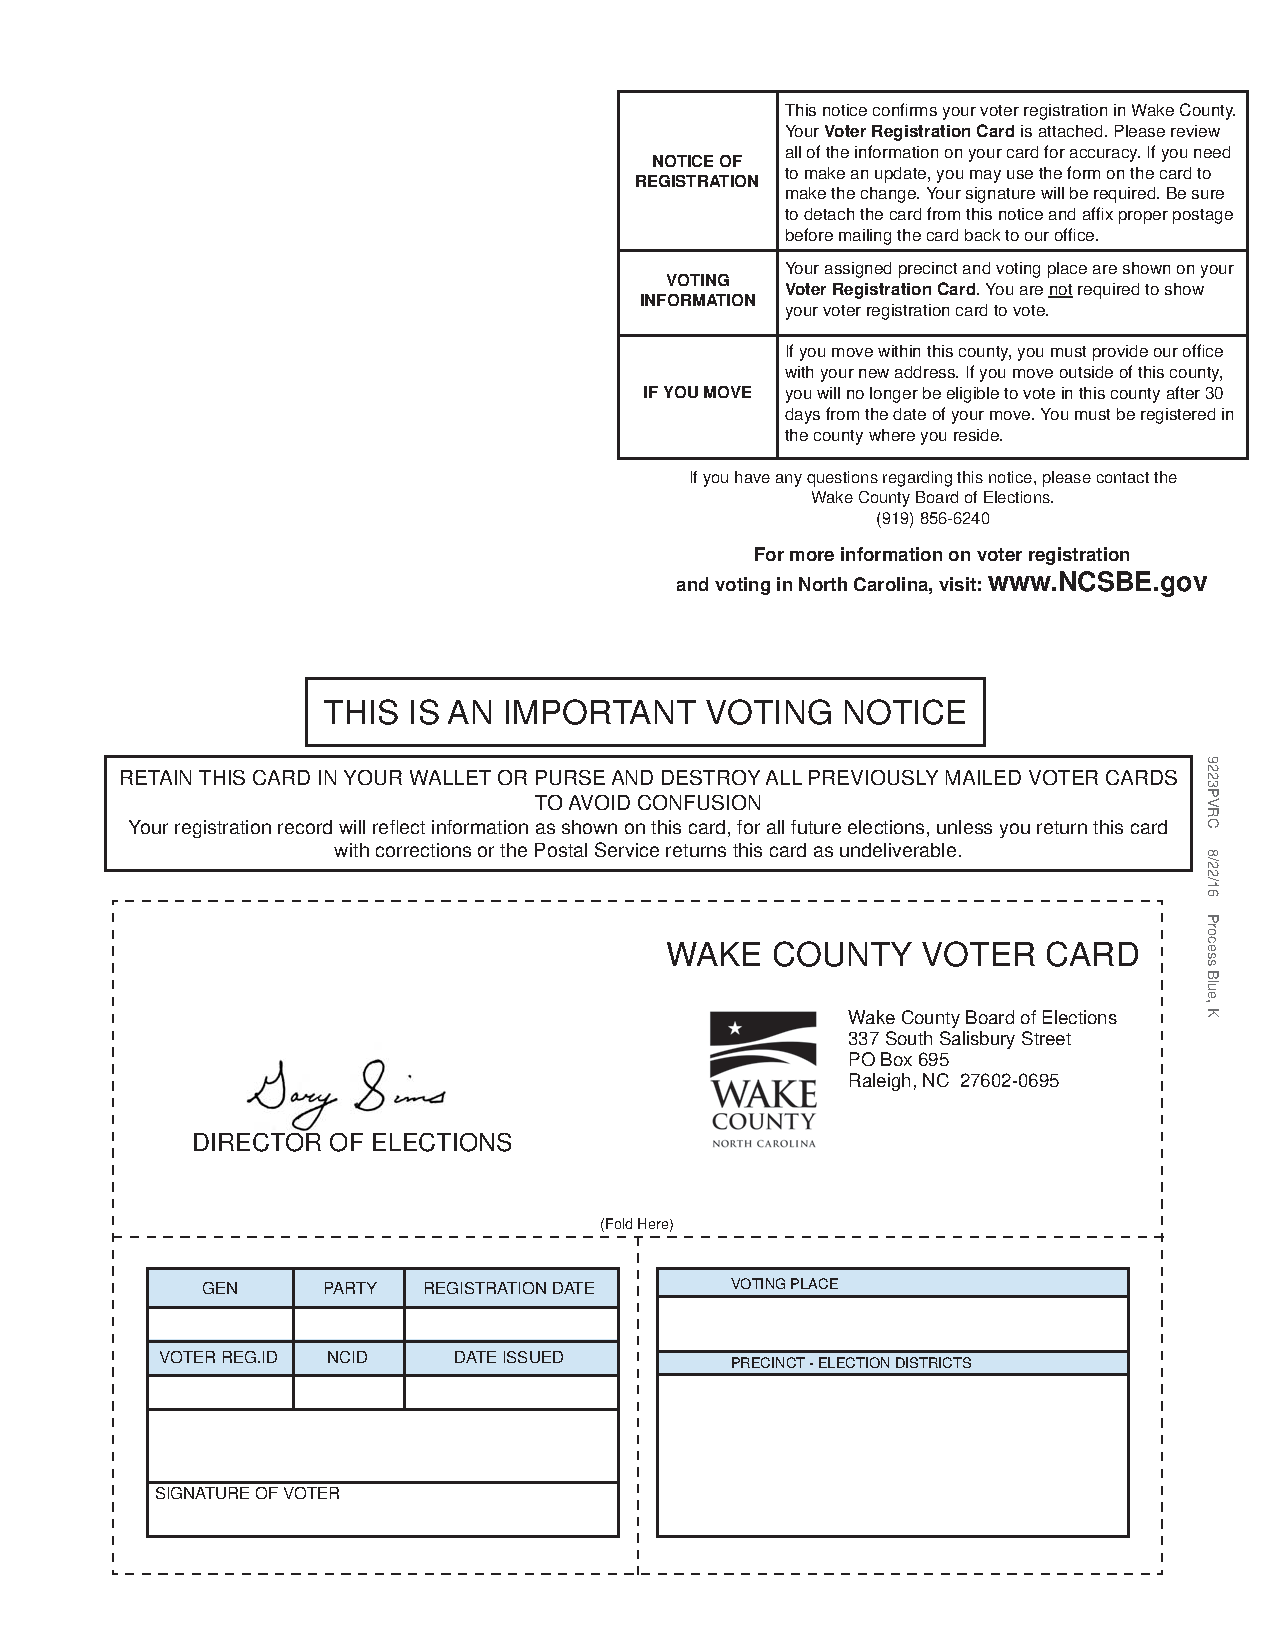
\includegraphics[width=5in, clip=true,  trim= 0in 0in 0in 0in ]{../../60_supplementary_materials/Mailer.pdf} }
	\label{figure_mailer}
	\end{center}
\end{figure}






%----------------------------------------------- APPENDIX C: FULL RESULTS ---------------------------------------------------%
\clearpage \newpage
\subsection{C. Full Results with Covariate Coefficients}\label{appendix_fullresults}
\setcounter{table}{0}
\setcounter{figure}{0}
\renewcommand{\thetable}{C\arabic{table}}
\renewcommand{\thefigure}{C\arabic{figure}}

This appendix presents the results from the main tables in the paper with the coefficient estimates for the control variables.  We omit those coefficients from the tables in the main tables in the paper for the sake of space.



% TABLE 4: Average Effect of Polling Place Changes and Drive Time Changes
%------------------------------------------------------------------------
\begin{table}[h!]\centering \scriptsize
\def\sym#1{\ifmmode^{#1}\else\(^{#1}\)\fi}
	\caption{The Average Effect of Polling Place Changes and Drive Time on Voter Turnout With Controls}\label{table_pp_panel_combined_wcontrols}
	\smallskip
	\begin{tabular}{@{\extracolsep{5pt}}l*{6}{c}}
	\noalign{\smallskip}\hline\hline\noalign{\smallskip}\noalign{\smallskip}
			&  \multicolumn{2}{c}{$Pr(VoteElecDay)$} &  \multicolumn{2}{c}{$Pr(VoteEarly)$} &  \multicolumn{2}{c}{$Pr(VoteAny)$}  \\
			\cline{2-3} \cline{4-5} \cline{6-7} \noalign{\smallskip}
				                &\multicolumn{1}{c}{(1)}         &\multicolumn{1}{c}{(2)}         &\multicolumn{1}{c}{(3)}         &\multicolumn{1}{c}{(4)}         &\multicolumn{1}{c}{(5)}         &\multicolumn{1}{c}{(6)}         \\
\midrule
$\Delta$\emph{PollingPlace} $(\hat{\beta})$&  -0.0073\sym{**} &  -0.0067\sym{*}  &   0.0063\sym{*}  &   0.0058         &  -0.0015         &  -0.0015         \\
                & (0.0037)         & (0.0037)         & (0.0037)         & (0.0038)         & (0.0015)         & (0.0016)         \\
\emph{Black}$\cdot 2016$&    0.076\sym{***}&    0.076\sym{***}&    -0.12\sym{***}&    -0.12\sym{***}&   -0.028\sym{***}&   -0.028\sym{***}\\
                & (0.0025)         & (0.0025)         & (0.0031)         & (0.0031)         & (0.0018)         & (0.0018)         \\
\emph{Hispanic}$\cdot 2016$&   -0.094\sym{***}&   -0.094\sym{***}&     0.14\sym{***}&     0.14\sym{***}&    0.040\sym{***}&    0.040\sym{***}\\
                &  (0.011)         &  (0.011)         &  (0.011)         &  (0.011)         & (0.0094)         & (0.0094)         \\
\emph{Unknown}$\cdot 2016$&   -0.063\sym{***}&   -0.063\sym{***}&    0.095\sym{***}&    0.095\sym{***}&    0.024\sym{***}&    0.024\sym{***}\\
                & (0.0043)         & (0.0043)         & (0.0048)         & (0.0048)         & (0.0040)         & (0.0040)         \\
\emph{Other}$\cdot 2016$&   -0.071\sym{***}&   -0.071\sym{***}&     0.14\sym{***}&     0.14\sym{***}&    0.060\sym{***}&    0.060\sym{***}\\
                & (0.0052)         & (0.0052)         & (0.0056)         & (0.0056)         & (0.0043)         & (0.0043)         \\
\emph{NativeAm}$\cdot 2016$&   -0.042\sym{***}&   -0.042\sym{***}&     0.11\sym{***}&     0.11\sym{***}&    0.070\sym{***}&    0.070\sym{***}\\
                &  (0.016)         &  (0.016)         &  (0.013)         &  (0.013)         &  (0.011)         &  (0.011)         \\
\emph{Asian}$\cdot 2016$&   -0.057\sym{***}&   -0.056\sym{***}&     0.14\sym{***}&     0.14\sym{***}&    0.068\sym{***}&    0.068\sym{***}\\
                & (0.0070)         & (0.0070)         & (0.0076)         & (0.0076)         & (0.0064)         & (0.0064)         \\
\emph{MultiRace}$\cdot 2016$&   -0.057\sym{***}&   -0.057\sym{***}&    0.083\sym{***}&    0.083\sym{***}&    0.018\sym{**} &    0.018\sym{**} \\
                & (0.0083)         & (0.0083)         & (0.0092)         & (0.0092)         & (0.0080)         & (0.0080)         \\
$\Delta$\emph{MuchCloser} $(\hat{\lambda})$&                  &    0.014         &                  &   -0.011         &                  &   0.0022         \\
                &                  &  (0.012)         &                  &  (0.013)         &                  & (0.0059)         \\
$\Delta$\emph{MuchFurther} $(\hat{\delta})$&                  &   -0.031\sym{**} &                  &    0.027\sym{*}  &                  &  -0.0026         \\
                &                  &  (0.014)         &                  &  (0.014)         &                  & (0.0054)         \\
\midrule
Individual FE   &\checkmark         &\checkmark         &\checkmark         &\checkmark         &\checkmark         &\checkmark         \\
Year FE         &\checkmark         &\checkmark         &\checkmark         &\checkmark         &\checkmark         &\checkmark         \\
County x Year FE&\checkmark         &\checkmark         &\checkmark         &\checkmark         &\checkmark         &\checkmark         \\
Year Sample     &Full Panel         &Full Panel         &Full Panel         &Full Panel         &Full Panel         &Full Panel         \\
Observations    &  4681792         &  4681792         &  4681792         &  4681792         &  4681792         &  4681792         \\
Mean of DV      &     0.30         &     0.30         &     0.46         &     0.46         &     0.80         &     0.80         \\
SD of DV        &     0.25         &     0.25         &     0.26         &     0.26         &     0.21         &     0.21         \\
 \\
	\noalign{\vspace*{-.10in}}\hline\hline\noalign{\smallskip}
\multicolumn{7}{p{5.2in}}{\scriptsize Standard errors clustered by precinct assignment history. } \\
\multicolumn{7}{l}{\scriptsize \sym{*} \(p<0.1\), \sym{**} \(p<0.05\), \sym{***} \(p<0.01\)}\\
\multicolumn{7}{p{5.2in}}{\scriptsize  \emph{Notes}: The table presents coefficients from estimating Equation~\ref{equation_traveltime_panel} both with and without the drive time indicators.  The unit of analysis is the voter-election.  This table presents the full covariates from Table \ref{table_pp_panel} in the paper.  The SD of the DV is the average of the within-$i$ standard deviations of the outcome variable. }
\end{tabular}
\end{table}






% TABLE 4: Polling Place Changes by Mode of Voting, Cross-Sectional, With Controls
%--------------------------------------------------------------------------------
\begin{table}[h!]\centering \scriptsize
\def\sym#1{\ifmmode^{#1}\else\(^{#1}\)\fi}
	\caption{The Average Effect of Polling Place Changes by Year With Covariate Coefficient Estimates}\label{table_pp_crosssec_wcontrols}
	\smallskip
	\begin{tabular}{@{\extracolsep{5pt}}l*{6}{c}}
	\noalign{\smallskip}\hline\hline\noalign{\smallskip}\noalign{\smallskip}
			&  \multicolumn{2}{c}{$Pr(VoteElecDay)$} &  \multicolumn{2}{c}{$Pr(VoteEarly)$} &  \multicolumn{2}{c}{$Pr(VoteAny)$}  \\
			\cline{2-3} \cline{4-5} \cline{6-7} \noalign{\smallskip}
				                &\multicolumn{1}{c}{(1)}         &\multicolumn{1}{c}{(2)}         &\multicolumn{1}{c}{(3)}         &\multicolumn{1}{c}{(4)}         &\multicolumn{1}{c}{(5)}         &\multicolumn{1}{c}{(6)}         \\
\midrule
$\Delta$\emph{PollingPlace} $(\hat{\beta})$&   -0.016\sym{***}&   -0.028\sym{***}&    0.019\sym{***}&    0.023\sym{***}&   0.0020         &  -0.0037\sym{**} \\
                & (0.0035)         & (0.0059)         & (0.0045)         & (0.0055)         & (0.0024)         & (0.0018)         \\
\emph{LagElecDayVoter}&     0.20\sym{***}&     0.37\sym{***}&   -0.053\sym{***}&     0.14\sym{***}&    0.096\sym{***}&     0.50\sym{***}\\
                & (0.0086)         & (0.0063)         & (0.0040)         & (0.0067)         &  (0.011)         &  (0.012)         \\
\emph{LagEarlyVoter}&    -0.15\sym{***}&    0.032\sym{***}&     0.32\sym{***}&     0.52\sym{***}&     0.13\sym{***}&     0.54\sym{***}\\
                & (0.0039)         & (0.0066)         & (0.0069)         & (0.0048)         &  (0.011)         &  (0.011)         \\
\emph{LagMailInVoter}&    -0.21\sym{***}&   -0.021\sym{***}&   -0.013\sym{*}  &     0.12\sym{***}&    0.031\sym{***}&     0.36\sym{***}\\
                & (0.0049)         & (0.0065)         & (0.0070)         & (0.0058)         & (0.0099)         &  (0.015)         \\
\emph{LagProvisionalVoter}&   -0.011         &     0.16\sym{***}&   -0.017         &     0.15\sym{***}&   -0.064\sym{***}&     0.32\sym{***}\\
                &  (0.016)         &  (0.012)         &  (0.011)         &  (0.012)         &  (0.017)         &  (0.014)         \\
\emph{Age}      &   0.0065\sym{***}&   0.0036\sym{***}&    0.023\sym{***}&    0.027\sym{***}&    0.027\sym{***}&    0.030\sym{***}\\
                &(0.00078)         &(0.00043)         &(0.00085)         & (0.0016)         & (0.0012)         & (0.0017)         \\
\emph{Age}$^{2}$&-0.000070\sym{***}&-0.000037\sym{***}& -0.00017\sym{***}& -0.00024\sym{***}& -0.00021\sym{***}& -0.00027\sym{***}\\
                &(0.0000072)         &(0.0000041)         &(0.0000074)         &(0.000014)         &(0.000010)         &(0.000015)         \\
\emph{Female}   &  -0.0079\sym{***}&  -0.0049\sym{***}&   0.0075\sym{***}&    0.018\sym{***}&   0.0036\sym{***}&    0.017\sym{***}\\
                & (0.0010)         & (0.0013)         & (0.0013)         & (0.0014)         & (0.0010)         &(0.00075)         \\
\emph{Black}    &   -0.090\sym{***}&   -0.010\sym{**} &     0.12\sym{***}&   -0.011\sym{**} &    0.024\sym{***}&   -0.029\sym{***}\\
                & (0.0056)         & (0.0049)         & (0.0056)         & (0.0043)         & (0.0030)         & (0.0039)         \\
\emph{Hispanic} &    0.049\sym{***}&   -0.029\sym{***}&    -0.17\sym{***}& -0.00025         &    -0.11\sym{***}&   -0.023\sym{**} \\
                &  (0.011)         & (0.0065)         & (0.0086)         & (0.0076)         & (0.0099)         & (0.0087)         \\
\emph{UnknownRace}&    0.024\sym{***}&   -0.018\sym{***}&    -0.16\sym{***}&   -0.032\sym{***}&    -0.13\sym{***}&   -0.047\sym{***}\\
                & (0.0058)         & (0.0043)         & (0.0045)         & (0.0042)         & (0.0066)         & (0.0049)         \\
\emph{OtherRace}&    0.044\sym{***}&  -0.0055         &    -0.15\sym{***}&  -0.0015         &    -0.10\sym{***}&  -0.0028         \\
                & (0.0057)         & (0.0078)         & (0.0037)         & (0.0052)         & (0.0054)         & (0.0061)         \\
\emph{NativeAm} &    0.074\sym{***}&    0.049\sym{***}&    -0.15\sym{***}&   -0.031\sym{***}&   -0.073\sym{***}&    0.023\sym{**} \\
                & (0.0072)         &  (0.016)         & (0.0063)         & (0.0079)         & (0.0072)         & (0.0094)         \\
\emph{Asian}    &    0.025\sym{***}&   -0.012         &    -0.18\sym{***}&  -0.0052         &    -0.14\sym{***}&   -0.012         \\
                & (0.0074)         & (0.0098)         &  (0.013)         &  (0.010)         &  (0.018)         &  (0.014)         \\
\emph{MultiRace}&  -0.0027         &   -0.031\sym{***}&    -0.14\sym{***}&   -0.026\sym{***}&    -0.13\sym{***}&   -0.051\sym{***}\\
                & (0.0063)         & (0.0046)         & (0.0062)         & (0.0058)         & (0.0081)         & (0.0061)         \\
\emph{Income}   &  -0.0021\sym{***}&  -0.0030\sym{**} &   0.0084\sym{***}&   0.0064\sym{***}&   0.0077\sym{***}&   0.0040\sym{***}\\
                &(0.00069)         & (0.0015)         &(0.00093)         & (0.0016)         &(0.00050)         &(0.00041)         \\
\emph{Republican}&  -0.0077\sym{***}&    0.028\sym{***}&    0.024\sym{***}&   -0.010\sym{*}  &    0.036\sym{***}&    0.021\sym{***}\\
                & (0.0019)         & (0.0041)         & (0.0035)         & (0.0061)         & (0.0024)         & (0.0029)         \\
\emph{Unaffiliated}&   -0.011\sym{***}&   0.0091\sym{***}&   -0.013\sym{***}&  -0.0059         &   -0.019\sym{***}&   0.0073\sym{***}\\
                & (0.0025)         & (0.0023)         & (0.0031)         & (0.0038)         & (0.0016)         & (0.0022)         \\
\emph{Libertarian}&  -0.0070         &    0.014         &   -0.055\sym{***}&   -0.034\sym{***}&   -0.058\sym{***}&   -0.016         \\
                &  (0.011)         & (0.0086)         &  (0.014)         & (0.0097)         &  (0.010)         &  (0.010)         \\
\midrule
County FE       &\checkmark         &\checkmark         &\checkmark         &\checkmark         &\checkmark         &\checkmark         \\
Year Sample     &     2012         &     2016         &     2012         &     2016         &     2012         &     2016         \\
Observations    &  2340293         &  2340293         &  2340293         &  2340293         &  2340293         &  2340293         \\
Mean of DV      &     0.33         &     0.26         &     0.47         &     0.45         &     0.84         &     0.75         \\
SD of DV        &     0.46         &     0.44         &     0.49         &     0.49         &     0.36         &     0.43         \\
 \\
	\noalign{\vspace*{-.10in}}\hline\hline\noalign{\smallskip}
  \multicolumn{7}{p{5.4in}}{\scriptsize Robust standard errors in parentheses. } \\
\multicolumn{7}{l}{\scriptsize \sym{*} \(p<0.1\), \sym{**} \(p<0.05\), \sym{***} \(p<0.01\)}\\
\multicolumn{7}{p{5.9in}}{\scriptsize  \emph{Notes}: The table presents coefficients from estimating Equation~\ref{equation_aggregate_crosssectional_closefurther} without the drive time indicators.  The unit of analysis is the voter.   The SD is the average of the within-county standard deviations of the outcome.  }
\end{tabular}
\end{table}



% TABLE 5: Travel Time Changes by Mode of Voting, Cross-Sectional With Controls
%------------------------------------------------------------------------------
\begin{table}[t!]\centering \scriptsize
\def\sym#1{\ifmmode^{#1}\else\(^{#1}\)\fi}
	\caption{The Average Effect of Changes in Travel Time to Polling Places by Year With Covariate Coefficient Estimates}\label{table_pp_crosssec_closerfurther_wcontrols}
	\smallskip
	\begin{tabular}{@{\extracolsep{5pt}}l*{6}{c}}
	\noalign{\smallskip}\hline\hline\noalign{\smallskip}\noalign{\smallskip}
			&  \multicolumn{2}{c}{$Pr(VoteElecDay)$} &  \multicolumn{2}{c}{$Pr(VoteEarly)$} &  \multicolumn{2}{c}{$Pr(VoteAny)$}  \\
			\cline{2-3} \cline{4-5} \cline{6-7} \noalign{\smallskip}
				                &\multicolumn{1}{c}{(1)}         &\multicolumn{1}{c}{(2)}         &\multicolumn{1}{c}{(3)}         &\multicolumn{1}{c}{(4)}         &\multicolumn{1}{c}{(5)}         &\multicolumn{1}{c}{(6)}         \\
\midrule
$\Delta$\emph{MuchCloser} $(\hat{\lambda})$&    0.017         &    0.026\sym{***}&   -0.013         &   -0.033\sym{***}&  0.00016         &  -0.0039         \\
                &  (0.015)         & (0.0087)         &  (0.014)         & (0.0093)         & (0.0048)         & (0.0050)         \\
$\Delta$\emph{MuchFurther} $(\hat{\delta})$&  -0.0077         &   -0.045\sym{***}&   0.0095         &    0.039\sym{**} &   0.0044         &  -0.0073         \\
                & (0.0075)         &  (0.016)         & (0.0075)         &  (0.019)         & (0.0048)         & (0.0045)         \\
$\Delta$\emph{PollingPlace} $(\hat{\beta})$&   -0.017\sym{***}&   -0.027\sym{***}&    0.019\sym{***}&    0.023\sym{***}&   0.0018         &  -0.0033\sym{*}  \\
                & (0.0034)         & (0.0055)         & (0.0045)         & (0.0051)         & (0.0025)         & (0.0018)         \\
\emph{LagElecDayVoter}&     0.20\sym{***}&     0.37\sym{***}&   -0.053\sym{***}&     0.14\sym{***}&    0.096\sym{***}&     0.50\sym{***}\\
                & (0.0086)         & (0.0063)         & (0.0040)         & (0.0067)         &  (0.011)         &  (0.012)         \\
\emph{LagEarlyVoter}&    -0.15\sym{***}&    0.032\sym{***}&     0.32\sym{***}&     0.52\sym{***}&     0.13\sym{***}&     0.54\sym{***}\\
                & (0.0039)         & (0.0066)         & (0.0069)         & (0.0048)         &  (0.011)         &  (0.011)         \\
\emph{LagMailInVoter}&    -0.21\sym{***}&   -0.021\sym{***}&   -0.013\sym{*}  &     0.12\sym{***}&    0.031\sym{***}&     0.36\sym{***}\\
                & (0.0049)         & (0.0065)         & (0.0070)         & (0.0058)         & (0.0099)         &  (0.015)         \\
\emph{LagProvisionalVoter}&   -0.011         &     0.16\sym{***}&   -0.017         &     0.15\sym{***}&   -0.064\sym{***}&     0.32\sym{***}\\
                &  (0.016)         &  (0.012)         &  (0.011)         &  (0.012)         &  (0.017)         &  (0.014)         \\
\emph{Age}      &   0.0065\sym{***}&   0.0036\sym{***}&    0.023\sym{***}&    0.027\sym{***}&    0.027\sym{***}&    0.030\sym{***}\\
                &(0.00078)         &(0.00043)         &(0.00085)         & (0.0016)         & (0.0012)         & (0.0017)         \\
\emph{Age}$^{2}$&-0.000070\sym{***}&-0.000037\sym{***}& -0.00017\sym{***}& -0.00024\sym{***}& -0.00021\sym{***}& -0.00027\sym{***}\\
                &(0.0000072)         &(0.0000041)         &(0.0000074)         &(0.000014)         &(0.000010)         &(0.000015)         \\
\emph{Female}   &  -0.0079\sym{***}&  -0.0049\sym{***}&   0.0075\sym{***}&    0.018\sym{***}&   0.0036\sym{***}&    0.017\sym{***}\\
                & (0.0010)         & (0.0013)         & (0.0013)         & (0.0014)         & (0.0010)         &(0.00075)         \\
\emph{Black}    &   -0.090\sym{***}&   -0.010\sym{**} &     0.12\sym{***}&   -0.011\sym{**} &    0.024\sym{***}&   -0.029\sym{***}\\
                & (0.0056)         & (0.0049)         & (0.0056)         & (0.0043)         & (0.0030)         & (0.0039)         \\
\emph{Hispanic} &    0.049\sym{***}&   -0.028\sym{***}&    -0.17\sym{***}& -0.00035         &    -0.11\sym{***}&   -0.023\sym{**} \\
                &  (0.011)         & (0.0065)         & (0.0086)         & (0.0076)         & (0.0098)         & (0.0087)         \\
\emph{UnknownRace}&    0.024\sym{***}&   -0.018\sym{***}&    -0.16\sym{***}&   -0.032\sym{***}&    -0.13\sym{***}&   -0.047\sym{***}\\
                & (0.0058)         & (0.0043)         & (0.0045)         & (0.0042)         & (0.0066)         & (0.0049)         \\
\emph{OtherRace}&    0.044\sym{***}&  -0.0054         &    -0.15\sym{***}&  -0.0015         &    -0.10\sym{***}&  -0.0028         \\
                & (0.0057)         & (0.0077)         & (0.0037)         & (0.0052)         & (0.0054)         & (0.0061)         \\
\emph{NativeAm} &    0.074\sym{***}&    0.048\sym{***}&    -0.15\sym{***}&   -0.030\sym{***}&   -0.073\sym{***}&    0.023\sym{**} \\
                & (0.0072)         &  (0.016)         & (0.0063)         & (0.0078)         & (0.0072)         & (0.0094)         \\
\emph{Asian}    &    0.025\sym{***}&   -0.012         &    -0.18\sym{***}&  -0.0052         &    -0.14\sym{***}&   -0.012         \\
                & (0.0074)         & (0.0098)         &  (0.013)         &  (0.011)         &  (0.018)         &  (0.014)         \\
\emph{MultiRace}&  -0.0028         &   -0.031\sym{***}&    -0.14\sym{***}&   -0.026\sym{***}&    -0.13\sym{***}&   -0.051\sym{***}\\
                & (0.0063)         & (0.0046)         & (0.0062)         & (0.0058)         & (0.0081)         & (0.0061)         \\
\emph{Income}   &  -0.0021\sym{***}&  -0.0030\sym{**} &   0.0084\sym{***}&   0.0064\sym{***}&   0.0077\sym{***}&   0.0040\sym{***}\\
                &(0.00068)         & (0.0015)         &(0.00092)         & (0.0016)         &(0.00050)         &(0.00041)         \\
\emph{Republican}&  -0.0077\sym{***}&    0.028\sym{***}&    0.024\sym{***}&   -0.010\sym{*}  &    0.036\sym{***}&    0.021\sym{***}\\
                & (0.0019)         & (0.0041)         & (0.0035)         & (0.0061)         & (0.0024)         & (0.0029)         \\
\emph{Unaffiliated}&   -0.011\sym{***}&   0.0091\sym{***}&   -0.013\sym{***}&  -0.0059         &   -0.019\sym{***}&   0.0073\sym{***}\\
                & (0.0025)         & (0.0023)         & (0.0031)         & (0.0038)         & (0.0016)         & (0.0022)         \\
\emph{Libertarian}&  -0.0070         &    0.014         &   -0.055\sym{***}&   -0.034\sym{***}&   -0.058\sym{***}&   -0.016         \\
                &  (0.011)         & (0.0086)         &  (0.014)         & (0.0097)         &  (0.010)         &  (0.010)         \\
\midrule
County FE       &\checkmark         &\checkmark         &\checkmark         &\checkmark         &\checkmark         &\checkmark         \\
Year Sample     &     2012         &     2016         &     2012         &     2016         &     2012         &     2016         \\
Observations    &  2340293         &  2340293         &  2340293         &  2340293         &  2340293         &  2340293         \\
Mean of DV      &     0.33         &     0.26         &     0.47         &     0.45         &     0.84         &     0.75         \\
SD of DV        &     0.46         &     0.44         &     0.49         &     0.49         &     0.36         &     0.43         \\
 \\
	\noalign{\vspace*{-.10in}}\hline\hline\noalign{\smallskip}
\multicolumn{7}{p{5.4in}}{\scriptsize Robust standard errors in parentheses. } \\
\multicolumn{7}{l}{\scriptsize \sym{*} \(p<0.1\), \sym{**} \(p<0.05\), \sym{***} \(p<0.01\)}\\
\multicolumn{7}{p{5.4in}}{\scriptsize  \emph{Notes}: The table presents coefficients from estimating Equation~\ref{equation_aggregate_crosssectional_closefurther}.  The unit of analysis is the voter.  The SD is the average of the within-county standard deviations of the outcome.}
\end{tabular}
\end{table}



% TABLE 6: Polling Place Changes by Mode of Voting, Cross-Sectional by Race with Controls
%----------------------------------------------------------------------------------------
\begin{table}[t!]\centering \scriptsize
\def\sym#1{\ifmmode^{#1}\else\(^{#1}\)\fi}
	\caption{The Differential Effects of Polling Place Changes by Race With Controls}\label{table_pp_panel_race_wcontrols}
	\smallskip
	\begin{tabular}{@{\extracolsep{5pt}}l*{6}{c}}
	\noalign{\smallskip}\hline\hline\noalign{\smallskip}\noalign{\smallskip}
			&  \multicolumn{2}{c}{$Pr(VoteElecDay)$} &  \multicolumn{2}{c}{$Pr(VoteEarly)$} &  \multicolumn{2}{c}{$Pr(VoteAny)$}  \\
			\cline{2-3} \cline{4-5} \cline{6-7} \noalign{\smallskip}
				                &\multicolumn{1}{c}{(1)}         &\multicolumn{1}{c}{(2)}         &\multicolumn{1}{c}{(3)}         &\multicolumn{1}{c}{(4)}         &\multicolumn{1}{c}{(5)}         &\multicolumn{1}{c}{(6)}         \\
\midrule
$\Delta$\emph{PollingPlace} $(\hat{\beta})$&  -0.0085\sym{**} &  -0.0077\sym{*}  &   0.0089\sym{**} &   0.0082\sym{**} & -0.00032         & -0.00041         \\
                & (0.0041)         & (0.0041)         & (0.0041)         & (0.0041)         & (0.0018)         & (0.0019)         \\
$\Delta PollingPlace \cdot$\emph{NonWhite}&   0.0048         &   0.0042         &   -0.010\sym{**} &  -0.0095\sym{*}  &  -0.0049         &  -0.0043         \\
                & (0.0044)         & (0.0045)         & (0.0052)         & (0.0053)         & (0.0030)         & (0.0031)         \\
\emph{Black}$\cdot 2016$&    0.076\sym{***}&    0.076\sym{***}&    -0.12\sym{***}&    -0.12\sym{***}&   -0.028\sym{***}&   -0.028\sym{***}\\
                & (0.0025)         & (0.0025)         & (0.0031)         & (0.0031)         & (0.0018)         & (0.0018)         \\
\emph{Hispanic}$\cdot 2016$&   -0.094\sym{***}&   -0.094\sym{***}&     0.14\sym{***}&     0.14\sym{***}&    0.040\sym{***}&    0.040\sym{***}\\
                &  (0.011)         &  (0.011)         &  (0.011)         &  (0.011)         & (0.0094)         & (0.0094)         \\
\emph{Unknown}$\cdot 2016$&   -0.063\sym{***}&   -0.063\sym{***}&    0.095\sym{***}&    0.095\sym{***}&    0.024\sym{***}&    0.024\sym{***}\\
                & (0.0043)         & (0.0043)         & (0.0048)         & (0.0048)         & (0.0040)         & (0.0040)         \\
\emph{Other}$\cdot 2016$&   -0.071\sym{***}&   -0.071\sym{***}&     0.14\sym{***}&     0.14\sym{***}&    0.060\sym{***}&    0.060\sym{***}\\
                & (0.0052)         & (0.0052)         & (0.0056)         & (0.0056)         & (0.0043)         & (0.0043)         \\
\emph{NativeAm}$\cdot 2016$&   -0.042\sym{***}&   -0.042\sym{***}&     0.11\sym{***}&     0.11\sym{***}&    0.070\sym{***}&    0.070\sym{***}\\
                &  (0.016)         &  (0.016)         &  (0.013)         &  (0.013)         &  (0.011)         &  (0.011)         \\
\emph{Asian}$\cdot 2016$&   -0.057\sym{***}&   -0.056\sym{***}&     0.14\sym{***}&     0.14\sym{***}&    0.068\sym{***}&    0.069\sym{***}\\
                & (0.0069)         & (0.0069)         & (0.0076)         & (0.0076)         & (0.0064)         & (0.0064)         \\
\emph{MultiRace}$\cdot 2016$&   -0.057\sym{***}&   -0.057\sym{***}&    0.083\sym{***}&    0.083\sym{***}&    0.018\sym{**} &    0.018\sym{**} \\
                & (0.0083)         & (0.0083)         & (0.0092)         & (0.0092)         & (0.0080)         & (0.0080)         \\
$\Delta$\emph{MuchCloser} $(\hat{\lambda})$&                  &    0.016         &                  &   -0.011         &                  &   0.0051         \\
                &                  &  (0.013)         &                  &  (0.014)         &                  & (0.0069)         \\
$\Delta$\emph{MuchFurther} $(\hat{\delta})$&                  &   -0.034\sym{**} &                  &    0.029\sym{*}  &                  &  -0.0021         \\
                &                  &  (0.015)         &                  &  (0.015)         &                  & (0.0058)         \\
$\Delta$\emph{MuchCloser}$\cdot NonWhite$&                  &   -0.011         &                  &  -0.0012         &                  &   -0.018         \\
                &                  &  (0.017)         &                  &  (0.016)         &                  &  (0.013)         \\
$\Delta$\emph{MuchFurther}$\cdot NonWhite$&                  &    0.017         &                  &   -0.022         &                  &  -0.0050         \\
                &                  &  (0.021)         &                  &  (0.019)         &                  &  (0.012)         \\
\midrule
Individual FE   &\checkmark         &\checkmark         &\checkmark         &\checkmark         &\checkmark         &\checkmark         \\
Year FE         &\checkmark         &\checkmark         &\checkmark         &\checkmark         &\checkmark         &\checkmark         \\
County x Year FE&\checkmark         &\checkmark         &\checkmark         &\checkmark         &\checkmark         &\checkmark         \\
Year Sample     &Full Panel         &Full Panel         &Full Panel         &Full Panel         &Full Panel         &Full Panel         \\
Observations    &  4681792         &  4681792         &  4681792         &  4681792         &  4681792         &  4681792         \\
Mean of DV      &     0.30         &     0.30         &     0.46         &     0.46         &     0.80         &     0.80         \\
SD of DV        &     0.25         &     0.25         &     0.26         &     0.26         &     0.21         &     0.21         \\
 \\
	\noalign{\vspace*{-.10in}}\hline\hline\noalign{\smallskip}
\multicolumn{7}{p{5.1in}}{\scriptsize Standard errors clustered by precinct assignment history. } \\
\multicolumn{7}{l}{\scriptsize \sym{*} \(p<0.1\), \sym{**} \(p<0.05\), \sym{***} \(p<0.01\)}\\
\multicolumn{7}{p{5.1in}}{\scriptsize  \emph{Notes}: The table presents coefficients from estimating Equation~\ref{equation_traveltime_panel} without the drive time indicators.  The unit of analysis is the voter-election.   This table presents the full covariates from Table ~\ref{table_pp_panel_race} in the paper.  The SD is the average of the within-$i$ standard deviations of the outcome.}
\end{tabular}
\end{table}






%------------------------------------------ APPENDIX D: RACE HETEROGENEITY ---------------------------------------------%
\clearpage \newpage
\subsection{D. Additional Racial Heterogeneity Specifications}\label{appendix_racehetero}
\setcounter{table}{0}
\setcounter{figure}{0}
\renewcommand{\thetable}{D\arabic{table}}
\renewcommand{\thefigure}{D\arabic{figure}}


\noindent In this appendix, we present additional results that examine heterogeneity in the effect of polling place changes by race. Table~\ref{table_pp_crosssec_closerfurther_nwhite} begins by showing that the effects of polling place changes by race do not vary by how those changes impact travel costs, nor are the results different in the panel analysis either overall (Table~\ref{table_pp_panel_race}) or depending on drive time (Table~\ref{table_pp_panel_closefurther_race}).  Finally, we present the main table polling place change table from the paper but with the non-white category broken out into each race indicator (Table~\ref{table_pp_crosssec_allraces}).  Because we observe no differential travel time effects for white as compared to non-white, and given the heinousness of a table with interactions across two distances for six races, we do not present the table for drive times interacted with each individual race.

Table~\ref{table_pp_crosssec_closerfurther_nwhite} examines different travel time changes by race.  We see no evidence that changes in travel time --- either increases or reductions --- under different partisan regimes differentially affected non-white voters.

% TABLE: Travel Time Changes by Mode of Voting, Cross-Sectional by Race
%-----------------------------------------------------------------------
\begin{table}[h!]\centering \scriptsize
\def\sym#1{\ifmmode^{#1}\else\(^{#1}\)\fi}
	\caption{The Differential Effects of Changes in Travel Time to Polling Places by Year and Race}\label{table_pp_crosssec_closerfurther_nwhite}
	\smallskip
	\begin{tabular}{@{\extracolsep{5pt}}l*{6}{c}}
	\noalign{\smallskip}\hline\hline\noalign{\smallskip}\noalign{\smallskip}
			&  \multicolumn{2}{c}{$Pr(VoteElecDay)$} &  \multicolumn{2}{c}{$Pr(VoteEarly)$} &  \multicolumn{2}{c}{$Pr(VoteAny)$}  \\
			\cline{2-3} \cline{4-5} \cline{6-7} \noalign{\smallskip}
				                &\multicolumn{1}{c}{(1)}         &\multicolumn{1}{c}{(2)}         &\multicolumn{1}{c}{(3)}         &\multicolumn{1}{c}{(4)}         &\multicolumn{1}{c}{(5)}         &\multicolumn{1}{c}{(6)}         \\
\midrule
$\Delta$\emph{PollingPlace} $(\hat{\beta})$&   -0.020\sym{***}&   -0.031\sym{***}&    0.022\sym{***}&    0.029\sym{***}&   0.0012         &  -0.0024         \\
                & (0.0042)         & (0.0059)         & (0.0051)         & (0.0055)         & (0.0026)         & (0.0019)         \\
$\Delta PollingPlace \cdot$\emph{NonWhite}&    0.014\sym{***}&    0.016\sym{***}&   -0.015\sym{**} &   -0.023\sym{***}&   0.0022         &  -0.0041         \\
                & (0.0049)         & (0.0048)         & (0.0063)         & (0.0053)         & (0.0037)         & (0.0034)         \\
\emph{NonWhite} &   -0.085\sym{***}&   -0.014\sym{***}&    0.091\sym{***}&   -0.011\sym{**} &  -0.0021         &   -0.032\sym{***}\\
                & (0.0044)         & (0.0041)         & (0.0045)         & (0.0043)         & (0.0029)         & (0.0034)         \\
$\Delta$\emph{MuchCloser} $(\hat{\lambda})$&    0.016         &    0.028\sym{***}&  -0.0095         &   -0.035\sym{***}&   0.0032         &  -0.0022         \\
                &  (0.016)         & (0.0098)         &  (0.014)         &  (0.010)         & (0.0048)         & (0.0057)         \\
$\Delta$\emph{MuchFurther} $(\hat{\delta})$&  -0.0087         &   -0.046\sym{***}&    0.011         &    0.040\sym{**} &   0.0047         &  -0.0065         \\
                & (0.0099)         &  (0.017)         & (0.0092)         &  (0.019)         & (0.0062)         & (0.0047)         \\
$\Delta$\emph{MuchCloser}$\cdot NonWhite$&   0.0084         &  -0.0022         &   -0.030\sym{*}  &  0.00041         &   -0.021         &  -0.0077         \\
                &  (0.015)         &  (0.021)         &  (0.017)         &  (0.013)         &  (0.013)         &  (0.016)         \\
$\Delta$\emph{MuchFurther}$\cdot NonWhite$&   0.0079         &    0.013         &  -0.0056         &   -0.025         &   0.0039         &  -0.0099         \\
                &  (0.018)         &  (0.017)         &  (0.026)         &  (0.017)         &  (0.017)         &  (0.012)         \\
\midrule
County FE       &\checkmark         &\checkmark         &\checkmark         &\checkmark         &\checkmark         &\checkmark         \\
Individual Controls&\checkmark         &\checkmark         &\checkmark         &\checkmark         &\checkmark         &\checkmark         \\
Year Sample     &     2012         &     2016         &     2012         &     2016         &     2012         &     2016         \\
Observations    &  2340293         &  2340293         &  2340293         &  2340293         &  2340293         &  2340293         \\
Mean of DV      &     0.33         &     0.26         &     0.47         &     0.45         &     0.84         &     0.75         \\
SD of DV        &     0.46         &     0.44         &     0.49         &     0.49         &     0.36         &     0.43         \\
 \\
	\noalign{\vspace*{-.10in}}\hline\hline\noalign{\smallskip}
\multicolumn{7}{p{5.2in}}{\scriptsize Robust standard errors in parentheses. } \\
\multicolumn{7}{l}{\scriptsize \sym{*} \(p<0.1\), \sym{**} \(p<0.05\), \sym{***} \(p<0.01\)}\\
\multicolumn{7}{p{5.2in}}{\scriptsize  \emph{Notes}: The table presents coefficients from estimating Equation~\ref{equation_aggregate_crosssectional_closefurther} with voter-race interactions.  The unit of analysis is the voter. The SD is the average of the within-county standard deviations of the outcome. }
\end{tabular}
\end{table}

Our panel results in Table~\ref{table_pp_panel_race} indicate that non-white voters are slightly more likely to continue voting on Election Day when they experience a polling place change, and less likely to vote early.  The net effect of this substitution is that they are less likely to turnout in general when they experience a polling place change.  The results in

% TABLE: Average Effect of Polling Place Changes, Race
%-----------------------------------------------------
\begin{table}[h!]\centering \scriptsize
\def\sym#1{\ifmmode^{#1}\else\(^{#1}\)\fi}
	\caption{The Average Effect of Polling Place Changes on Voter Turnout by Race}\label{table_pp_panel_race}
	\smallskip
	\begin{tabular}{@{\extracolsep{5pt}}l*{4}{c}}
	\noalign{\smallskip}\hline\hline\noalign{\smallskip}\noalign{\smallskip}
			&  \multicolumn{1}{c}{$Pr(VoteElecDay)$} &  \multicolumn{1}{c}{$Pr(VoteEarly)$} &  \multicolumn{1}{c}{$Pr(VoteAny)$}  \\
			\cline{2-4}  \noalign{\smallskip}
				                &\multicolumn{1}{c}{(1)}         &\multicolumn{1}{c}{(2)}         &\multicolumn{1}{c}{(3)}         \\
\midrule
$\Delta$\emph{PollingPlace} $(\hat{\beta})$&  -0.0085\sym{**} &   0.0089\sym{**} & -0.00032         \\
                & (0.0041)         & (0.0041)         & (0.0018)         \\
$\Delta PollingPlace \cdot$\emph{NonWhite}&   0.0048         &   -0.010\sym{**} &  -0.0049         \\
                & (0.0044)         & (0.0052)         & (0.0030)         \\
\midrule
Individual FE   &\checkmark         &\checkmark         &\checkmark         \\
Year FE         &\checkmark         &\checkmark         &\checkmark         \\
County x Year FE&\checkmark         &\checkmark         &\checkmark         \\
Race x Year FE  &\checkmark         &\checkmark         &\checkmark         \\
Year Sample     &Full Panel         &Full Panel         &Full Panel         \\
Observations    &  4681792         &  4681792         &  4681792         \\
Mean of DV      &     0.30         &     0.46         &     0.80         \\
SD of DV        &     0.25         &     0.26         &     0.21         \\
 \\
	\noalign{\vspace*{-.10in}}\hline\hline\noalign{\smallskip}
\multicolumn{4}{p{4.4in}}{\scriptsize Standard errors clustered by precinct assignment history. } \\
\multicolumn{4}{l}{\scriptsize \sym{*} \(p<0.1\), \sym{**} \(p<0.05\), \sym{***} \(p<0.01\)}\\
\multicolumn{4}{p{4.4in}}{\scriptsize  \emph{Notes}: The table presents coefficients from estimating Equation~\ref{equation_traveltime_panel} without the travel time indicators.  The unit of analysis is the voter-election. The SD is the average of the within-$i$ standard deviations of the outcome. }
\end{tabular}
\end{table}



% TABLE: Polling Place Changes and Travel Costs by Mode of Voting by Race
%------------------------------------------------------------------------
\begin{table}[h!]\centering \scriptsize
\def\sym#1{\ifmmode^{#1}\else\(^{#1}\)\fi}
	\caption{The Average Effect of Changes in Travel Time to Polling Place on Turnout by Race}\label{table_pp_panel_closefurther_race}
	\smallskip
	\begin{tabular}{@{\extracolsep{5pt}}l*{4}{c}}
	\noalign{\smallskip}\hline\hline\noalign{\smallskip}\noalign{\smallskip}
			&  \multicolumn{1}{c}{$Pr(VoteElecDay)$} &  \multicolumn{1}{c}{$Pr(VoteEarly)$} &  \multicolumn{1}{c}{$Pr(VoteAny)$}  \\
			\cline{2-4}  \noalign{\smallskip}
				                &\multicolumn{1}{c}{(1)}         &\multicolumn{1}{c}{(2)}         &\multicolumn{1}{c}{(3)}         \\
\midrule
$\Delta$\emph{PollingPlace} $(\hat{\beta})$&  -0.0077\sym{*}  &   0.0082\sym{**} & -0.00041         \\
                & (0.0041)         & (0.0041)         & (0.0019)         \\
$\Delta PollingPlace \cdot$\emph{NonWhite}&   0.0042         &  -0.0095\sym{*}  &  -0.0043         \\
                & (0.0045)         & (0.0053)         & (0.0031)         \\
$\Delta$\emph{MuchCloser} $(\hat{\lambda})$&    0.016         &   -0.011         &   0.0051         \\
                &  (0.013)         &  (0.014)         & (0.0069)         \\
$\Delta$\emph{MuchFurther} $(\hat{\delta})$&   -0.034\sym{**} &    0.029\sym{*}  &  -0.0021         \\
                &  (0.015)         &  (0.015)         & (0.0058)         \\
$\Delta$\emph{MuchCloser}$\cdot NonWhite$&   -0.011         &  -0.0012         &   -0.018         \\
                &  (0.017)         &  (0.016)         &  (0.013)         \\
$\Delta$\emph{MuchFurther}$\cdot NonWhite$&    0.017         &   -0.022         &  -0.0050         \\
                &  (0.021)         &  (0.019)         &  (0.012)         \\
\midrule
Individual FE   &\checkmark         &\checkmark         &\checkmark         \\
Year FE         &\checkmark         &\checkmark         &\checkmark         \\
County x Year FE&\checkmark         &\checkmark         &\checkmark         \\
Race x Year FE  &\checkmark         &\checkmark         &\checkmark         \\
Year Sample     &Full Panel         &Full Panel         &Full Panel         \\
Observations    &  4681792         &  4681792         &  4681792         \\
Mean of DV      &     0.30         &     0.46         &     0.80         \\
SD of DV        &     0.25         &     0.26         &     0.21         \\
 \\
	\noalign{\vspace*{-.10in}}\hline\hline\noalign{\smallskip}
\multicolumn{4}{p{4.3in}}{\scriptsize Standard errors clustered by precinct assignment history. } \\
\multicolumn{4}{l}{\scriptsize \sym{*} \(p<0.1\), \sym{**} \(p<0.05\), \sym{***} \(p<0.01\)}\\
\multicolumn{4}{p{4.3in}}{\scriptsize  \emph{Notes}: The table presents coefficients from estimating Equation~\ref{equation_traveltime_panel}.  The unit of analysis is the voter-election. The SD is the average of the within-$i$ standard deviations of the outcome. }
\end{tabular}
\end{table}


We note that there is little consistent evidence that our results for non-white vary meaningfully by specific races.  We might be interested in whether the effects for black are distinct from other races that are a smaller part of the population or have a less fraught history with voting rights in North Carolina.  But Table~\ref{table_pp_crosssec_allraces} provides little evidence of this.



% TABLE 6: Polling Place Changes by Mode of Voting, Cross-Sectional by Race ALL RACES
%-------------------------------------------------------------------------------------
\begin{table}[t!]\centering \scriptsize
\def\sym#1{\ifmmode^{#1}\else\(^{#1}\)\fi}
	\caption{The Differential Effects of Polling Place Changes by Year and Race}\label{table_pp_crosssec_allraces}
	\smallskip
	\begin{tabular}{@{\extracolsep{5pt}}l*{6}{c}}
	\noalign{\smallskip}\hline\hline\noalign{\smallskip}\noalign{\smallskip}
			&  \multicolumn{2}{c}{$Pr(VoteElecDay)$} &  \multicolumn{2}{c}{$Pr(VoteEarly)$} &  \multicolumn{2}{c}{$Pr(VoteAny)$}  \\
			\cline{2-3} \cline{4-5} \cline{6-7} \noalign{\smallskip}
				                &\multicolumn{1}{c}{(1)}         &\multicolumn{1}{c}{(2)}         &\multicolumn{1}{c}{(3)}         &\multicolumn{1}{c}{(4)}         &\multicolumn{1}{c}{(5)}         &\multicolumn{1}{c}{(6)}         \\
\midrule
$\Delta$\emph{PollingPlace} $(\hat{\beta})$&   -0.020\sym{***}&   -0.032\sym{***}&    0.023\sym{***}&    0.029\sym{***}&   0.0017         &  -0.0026         \\
                & (0.0044)         & (0.0063)         & (0.0053)         & (0.0060)         & (0.0024)         & (0.0019)         \\
$\Delta$\emph{PollingPlace}$\cdot Hispanic$&    0.025         &    0.028\sym{*}  &   -0.011         &  -0.0016         &    0.010         &    0.014         \\
                &  (0.019)         &  (0.016)         &  (0.015)         &  (0.018)         &  (0.014)         &  (0.012)         \\
$\Delta$\emph{PollingPlace}$\cdot Black$&    0.013\sym{**} &    0.018\sym{***}&   -0.015\sym{**} &   -0.026\sym{***}&  0.00023         &  -0.0052         \\
                & (0.0056)         & (0.0054)         & (0.0069)         & (0.0059)         & (0.0033)         & (0.0033)         \\
$\Delta$\emph{PollingPlace}$\cdot Unknown$&    0.017\sym{**} &  -0.0062         &   -0.017         &   0.0050         &   0.0030         &   0.0017         \\
                & (0.0075)         &  (0.011)         &  (0.012)         & (0.0098)         &  (0.011)         & (0.0077)         \\
$\Delta$\emph{PollingPlace}$\cdot Other$&  -0.0036         &   -0.011         & -0.00098         &   0.0085         &  -0.0068         &  -0.0019         \\
                & (0.0066)         & (0.0077)         &  (0.012)         & (0.0100)         & (0.0083)         & (0.0080)         \\
$\Delta$\emph{PollingPlace}$\cdot NativeAm$&    0.011         &   -0.012         &    0.015         &    0.021         &    0.028         &   0.0055         \\
                &  (0.022)         &  (0.027)         &  (0.017)         &  (0.026)         &  (0.025)         & (0.0093)         \\
$\Delta$\emph{PollingPlace}$\cdot Asian$&   0.0064         &  -0.0061         &   0.0062         &    0.028\sym{**} &    0.023         &    0.013         \\
                &  (0.010)         &  (0.010)         &  (0.024)         &  (0.013)         &  (0.019)         &  (0.014)         \\
$\Delta$\emph{PollingPlace}$\cdot MultiRace$&  -0.0030         &   0.0019         &   -0.019         &  -0.0071         &  -0.0097         &  -0.0027         \\
                &  (0.012)         &  (0.012)         &  (0.015)         &  (0.016)         &  (0.018)         &  (0.016)         \\
\emph{Black}    &   -0.092\sym{***}&   -0.013\sym{**} &     0.13\sym{***}&  -0.0067         &    0.024\sym{***}&   -0.028\sym{***}\\
                & (0.0054)         & (0.0050)         & (0.0056)         & (0.0044)         & (0.0031)         & (0.0040)         \\
\emph{UnknownRace}&    0.021\sym{***}&   -0.017\sym{***}&    -0.15\sym{***}&   -0.033\sym{***}&    -0.13\sym{***}&   -0.048\sym{***}\\
                & (0.0055)         & (0.0051)         & (0.0053)         & (0.0045)         & (0.0076)         & (0.0055)         \\
\emph{OtherRace}&    0.044\sym{***}&  -0.0038         &    -0.15\sym{***}&  -0.0027         &    -0.10\sym{***}&  -0.0025         \\
                & (0.0056)         & (0.0081)         & (0.0047)         & (0.0058)         & (0.0056)         & (0.0059)         \\
\emph{NativeAm} &    0.073\sym{***}&    0.050\sym{***}&    -0.15\sym{***}&   -0.034\sym{***}&   -0.078\sym{***}&    0.022\sym{**} \\
                & (0.0063)         &  (0.017)         & (0.0067)         & (0.0091)         & (0.0048)         & (0.0095)         \\
\emph{Asian}    &    0.024\sym{***}&   -0.011         &    -0.18\sym{***}&  -0.0093         &    -0.14\sym{***}&   -0.014         \\
                & (0.0077)         &  (0.011)         &  (0.016)         &  (0.012)         &  (0.020)         &  (0.015)         \\
\emph{MultiRace}&  -0.0023         &   -0.031\sym{***}&    -0.13\sym{***}&   -0.025\sym{***}&    -0.13\sym{***}&   -0.050\sym{***}\\
                & (0.0066)         & (0.0053)         & (0.0075)         & (0.0064)         & (0.0100)         & (0.0071)         \\
\emph{Hispanic} &    0.045\sym{***}&   -0.033\sym{***}&    -0.16\sym{***}&-0.000079         &    -0.11\sym{***}&   -0.025\sym{***}\\
                &  (0.011)         & (0.0068)         & (0.0091)         & (0.0087)         &  (0.010)         & (0.0088)         \\
\midrule
County FE       &\checkmark         &\checkmark         &\checkmark         &\checkmark         &\checkmark         &\checkmark         \\
Individual Controls&\checkmark         &\checkmark         &\checkmark         &\checkmark         &\checkmark         &\checkmark         \\
Year Sample     &     2012         &     2016         &     2012         &     2016         &     2012         &     2016         \\
Observations    &  2340293         &  2340293         &  2340293         &  2340293         &  2340293         &  2340293         \\
Mean of DV      &     0.33         &     0.26         &     0.47         &     0.45         &     0.84         &     0.75         \\
SD of DV        &     0.46         &     0.44         &     0.49         &     0.49         &     0.36         &     0.43         \\
 \\
	\noalign{\vspace*{-.10in}}\hline\hline\noalign{\smallskip}
\multicolumn{7}{p{5.6in}}{\scriptsize Robust standard errors in parentheses. } \\
\multicolumn{7}{l}{\scriptsize \sym{*} \(p<0.1\), \sym{**} \(p<0.05\), \sym{***} \(p<0.01\)}\\
\multicolumn{7}{p{5.6in}}{\scriptsize  \emph{Notes}: The table presents coefficients from estimating Equation~\ref{equation_aggregate_crosssectional_closefurther} without the travel time indicators but with $\Delta PollingPlace$ interacted with voter race.  The unit of analysis is the voter. The SD is the average of the within-county standard deviations of the outcome. }
\end{tabular}
\end{table}






%--------------------------------------- APPENDIX E: ALTERNATIVE TRAVEL TIME ------------------------------------------%
\clearpage \newpage
\subsection{E. Alternative Travel Time Changes Specifications}\label{appendix_traveltime}
\setcounter{table}{0}
\setcounter{figure}{0}
\renewcommand{\thetable}{E\arabic{table}}
\renewcommand{\thefigure}{E\arabic{figure}}


\noindent In the main paper we probe the effect of changes in the costs associated with traveling to the polls by estimating a model in which we compare level differences between those people moved more than 5 minutes closer or more than 5 minutes further from their polling place to those who had a smaller move (regardless of whether that move was closer or further).

In this appendix, we present additional results that model the relationship between changing drive time to polling place and voter turnout differently.  Specifically, we estimate a model similar to the model from the main paper (in which we trichotomize travel time changes into 5+ minutes closer, 5+ minutes further, and under 5 minutes closer or further) but allow the slope of the effects in those bins to vary.  That is, we interact the indicators for the general distance of a move with drive time change.  As compared to the main results in the paper, this accounts both for intercept differences and linear slope differences.

The results are presented in Table~\ref{table_pp_panel_closefurther_linear}. The excluded category are people who experience a polling place change of under 5 minutes (whether closer or further; this is why $\delta DriveTime$ is not included in the regression). We find that there is a differential linear slope in the effect of polling place change when voters are moved much further away.  The slope of the effect for Election Day voting is more negative relative to those who had smaller changes, and the slope of the effect for early voting is more positive.  These results indicate that the effect of a change in drive time does depend on whether that change is large or small when it comes to the choice of mode of vote.   However, critically, there is no differential overall turnout effect.



\vspace{.2in}
% TABLE: Polling Place Changes and Travel Costs by Mode of Voting
%----------------------------------------------------------------
\begin{table}[h!]\centering \scriptsize
\def\sym#1{\ifmmode^{#1}\else\(^{#1}\)\fi}
	\caption{The Average Effect of Changes in Travel Time to Polling Place on Turnout Using Linear Fits}\label{table_pp_panel_closefurther_linear}
	\smallskip
	\begin{tabular}{@{\extracolsep{5pt}}l*{4}{c}}
	\noalign{\smallskip}\hline\hline\noalign{\smallskip}\noalign{\smallskip}
			&  \multicolumn{1}{c}{$Pr(VoteElecDay)$} &  \multicolumn{1}{c}{$Pr(VoteEarly)$} &  \multicolumn{1}{c}{$Pr(VoteAny)$}  \\
			\cline{2-4}  \noalign{\smallskip}
				                &\multicolumn{1}{c}{(1)}         &\multicolumn{1}{c}{(2)}         &\multicolumn{1}{c}{(3)}         \\
\midrule
$\Delta$\emph{PollingPlace} $(\hat{\beta})$&   0.0029         &  -0.0087         &  -0.0075         \\
                &  (0.025)         &  (0.033)         &  (0.017)         \\
$\Delta$\emph{Closer}&   -0.014         &    0.018         &   0.0044         \\
                &  (0.025)         &  (0.033)         &  (0.016)         \\
$\Delta$\emph{Closer}$\cdot \Delta DriveTime$&  -0.0024         &   0.0017         & -0.00077         \\
                & (0.0018)         & (0.0022)         &(0.00091)         \\
$\Delta$\emph{Further}&  -0.0017         &   0.0073         &   0.0066         \\
                &  (0.024)         &  (0.032)         &  (0.016)         \\
$\Delta$\emph{Further}$\cdot \Delta DriveTime$&  -0.0053\sym{**} &   0.0046\sym{**} & -0.00025         \\
                & (0.0022)         & (0.0021)         &(0.00080)         \\
\midrule
Individual FE   &\checkmark         &\checkmark         &\checkmark         \\
Year FE         &\checkmark         &\checkmark         &\checkmark         \\
County x Year FE&\checkmark         &\checkmark         &\checkmark         \\
Race x Year FE  &\checkmark         &\checkmark         &\checkmark         \\
Year Sample     &Full Panel         &Full Panel         &Full Panel         \\
Observations    &  4681792         &  4681792         &  4681792         \\
Mean of DV      &     0.30         &     0.46         &     0.80         \\
SD of DV        &     0.25         &     0.26         &     0.21         \\
 \\
	\noalign{\vspace*{-.10in}}\hline\hline\noalign{\smallskip}
\multicolumn{4}{p{4.0in}}{\scriptsize Standard errors clustered by precinct assignment history. } \\
\multicolumn{4}{l}{\scriptsize \sym{*} \(p<0.1\), \sym{**} \(p<0.05\), \sym{***} \(p<0.01\)}\\
\multicolumn{4}{p{4.0in}}{\scriptsize  \emph{Notes}: The table presents coefficients from estimating Equation~\ref{equation_traveltime_panel} with additional interactions.  The unit of analysis is the voter-election.  The SD is the average of the within-$i$ standard deviations of the outcome. (either closer or further) }
\end{tabular}
\end{table}


In Table~\ref{table_pp_panel_closefurther_quadratic} we further allow the relationship between turnout and drive time to be non-linear -- specifically, to follow a quadratic functional form.  We do not find differential qualitative evidence that turnout changes as a (quadratic) function of the drive time to the new polling place.  The joint significance of the linear and quadratic terms for either the closer interactions or the further interactions are not significant.  Overall, the table suggests that differential linearity within the 5 minute bins constructed by our dummy accounts well for the relationship.


\vspace{.2in}
% TABLE: Polling Place Changes and Travel Costs by Mode of Voting
%----------------------------------------------------------------
\begin{table}[h!]\centering \scriptsize
\def\sym#1{\ifmmode^{#1}\else\(^{#1}\)\fi}
	\caption{The Average Effect of Changes in Travel Time to Polling Place on Turnout Using Quadratic Fits}\label{table_pp_panel_closefurther_quadratic}
	\smallskip
	\begin{tabular}{@{\extracolsep{5pt}}l*{4}{c}}
	\noalign{\smallskip}\hline\hline\noalign{\smallskip}\noalign{\smallskip}
			&  \multicolumn{1}{c}{$Pr(VoteElecDay)$} &  \multicolumn{1}{c}{$Pr(VoteEarly)$} &  \multicolumn{1}{c}{$Pr(VoteAny)$}  \\
			\cline{2-4}  \noalign{\smallskip}
				                &\multicolumn{1}{c}{(1)}         &\multicolumn{1}{c}{(2)}         &\multicolumn{1}{c}{(3)}         \\
\midrule
$\Delta$\emph{PollingPlace} $(\hat{\beta})$&  -0.0020         &  -0.0027         &  -0.0067         \\
                &  (0.025)         &  (0.033)         &  (0.017)         \\
$\Delta$\emph{Closer}&  -0.0099         &    0.015         &   0.0052         \\
                &  (0.025)         &  (0.033)         &  (0.016)         \\
$\Delta$\emph{Closer}$\cdot \Delta DriveTime$&  -0.0035         &   0.0046         &  0.00078         \\
                & (0.0032)         & (0.0040)         & (0.0018)         \\
$\Delta$\emph{Closer}$\cdot \Delta DriveTime^{2}$& -0.00013         &  0.00034         &  0.00018         \\
                &(0.00030)         &(0.00046)         &(0.00018)         \\
$\Delta$\emph{Further}& -0.00066         &   0.0045         &   0.0050         \\
                &  (0.024)         &  (0.032)         &  (0.016)         \\
$\Delta$\emph{Further}$\cdot \Delta DriveTime$&  -0.0015         &   0.0016         &  0.00050         \\
                & (0.0040)         & (0.0036)         & (0.0017)         \\
$\Delta$\emph{Further}$\cdot \Delta DriveTime^{2}$& -0.00042         &  0.00034         &-0.000084         \\
                &(0.00047)         &(0.00038)         &(0.00017)         \\
\midrule
Individual FE   &\checkmark         &\checkmark         &\checkmark         \\
Year FE         &\checkmark         &\checkmark         &\checkmark         \\
County x Year FE&\checkmark         &\checkmark         &\checkmark         \\
Race x Year FE  &\checkmark         &\checkmark         &\checkmark         \\
Year Sample     &Full Panel         &Full Panel         &Full Panel         \\
Observations    &  4681792         &  4681792         &  4681792         \\
Mean of DV      &     0.30         &     0.46         &     0.80         \\
SD of DV        &     0.25         &     0.26         &     0.21         \\
 \\
	\noalign{\vspace*{-.10in}}\hline\hline\noalign{\smallskip}
\multicolumn{4}{p{4.0in}}{\scriptsize Standard errors clustered by precinct assignment history. } \\
\multicolumn{4}{l}{\scriptsize \sym{*} \(p<0.1\), \sym{**} \(p<0.05\), \sym{***} \(p<0.01\)}\\
\multicolumn{4}{p{4.2in}}{\scriptsize  \emph{Notes}: The table presents coefficients from estimating Equation~\ref{equation_traveltime_panel} with additional interactions.  The unit of analysis is the voter-election.  The SD is the average of the within-$i$ standard deviations of the outcome.  The excluded category are voters who had their polling place moved under five minutes from them (either closer or further). }
\end{tabular}
\end{table}



We also estimate a specification that restricts the sample of voters to those who experience a polling place change of less than 10 minutes closer and less than 10 minutes further away.  This restriction better reflects what we plot in the scatter plots of the relationship between drive time and turnout.  And it also reflects the fact that there are extremely few observations in these far tails of the distribution.  And given that we use OLS, we want to be sensitive to the effect that extreme outliers might have on our results.


Table~\ref{table_pp_panel_closefurther_restricted} presents our results for the restricted sample.  These are slightly smaller in magnitude, and less significant than the results in the paper.  But the sign and pattern of magnitudes is very similar.



\vspace{.2in}
% TABLE: Polling Place Changes and Travel Costs by Mode of Voting for the Restricted Sample
%-------------------------------------------------------------------------------------------
\begin{table}[h!]\centering \scriptsize
\def\sym#1{\ifmmode^{#1}\else\(^{#1}\)\fi}
	\caption{The Average Effect of Changes in Travel Time to Polling Place on Turnout for the Restricted Sample}\label{table_pp_panel_closefurther_restricted}
	\smallskip
	\begin{tabular}{@{\extracolsep{5pt}}l*{4}{c}}
	\noalign{\smallskip}\hline\hline\noalign{\smallskip}\noalign{\smallskip}
			&  \multicolumn{1}{c}{$Pr(VoteElecDay)$} &  \multicolumn{1}{c}{$Pr(VoteEarly)$} &  \multicolumn{1}{c}{$Pr(VoteAny)$}  \\
			\cline{2-4}  \noalign{\smallskip}
				                &\multicolumn{1}{c}{(1)}         &\multicolumn{1}{c}{(2)}         &\multicolumn{1}{c}{(3)}         \\
\midrule
$\Delta$\emph{MuchCloser} $(\hat{\lambda})$&    0.016         &   -0.018         &  -0.0022         \\
                &  (0.013)         &  (0.012)         & (0.0056)         \\
$\Delta$\emph{MuchFurther} $(\hat{\delta})$&   -0.026\sym{**} &    0.022\sym{*}  &  -0.0028         \\
                &  (0.013)         &  (0.013)         & (0.0055)         \\
$\Delta$\emph{PollingPlace} $(\hat{\beta})$&  -0.0070\sym{*}  &   0.0062\sym{*}  &  -0.0015         \\
                & (0.0037)         & (0.0038)         & (0.0016)         \\
\midrule
Individual FE   &\checkmark         &\checkmark         &\checkmark         \\
Year FE         &\checkmark         &\checkmark         &\checkmark         \\
County x Year FE&\checkmark         &\checkmark         &\checkmark         \\
Race x Year FE  &\checkmark         &\checkmark         &\checkmark         \\
Year Sample     &Full Panel         &Full Panel         &Full Panel         \\
Observations    &  4675138         &  4675138         &  4675138         \\
Mean of DV      &     0.30         &     0.46         &     0.80         \\
SD of DV        &     0.25         &     0.26         &     0.21         \\
 \\
	\noalign{\vspace*{-.10in}}\hline\hline\noalign{\smallskip}
\multicolumn{4}{p{4.0in}}{\scriptsize Standard errors clustered by precinct assignment history. } \\
\multicolumn{4}{l}{\scriptsize \sym{*} \(p<0.1\), \sym{**} \(p<0.05\), \sym{***} \(p<0.01\)}\\
\multicolumn{4}{p{4.0in}}{\scriptsize  \emph{Notes}: The table presents coefficients from estimating Equation~\ref{equation_traveltime_panel}.  The unit of analysis is the voter-election.   The sample is restricted to those individuals in our sample who experienced drive time changes of less than 10 minutes closer or further away.  The SD is the average of the within-$i$ standard deviations of the outcome.}
\end{tabular}
\end{table}


Finally, we note that our results are robust to other models that readers might think capture the relationship between drive time and turnout --- specifically, models that simply dichotomize the closer/further relationship and model that relationship as linear, and models that dichotomize but model the model relationship as quadratic.  We do not present these results for the sake of space, but they are available upon request.  By robust, we mean that we find slightly more evidence of substitution when people are moved further from their polling place (as compared to closer), but that these substitution effects offset such that there is no differential overall turnout effect conditional on drive time.



%------------------------------------------ APPENDIX F: COUNTY-SPECIFIC -----------------------------------------%
\clearpage \newpage
\subsection{F. Individual County Estimates}\label{appendix_county}
\setcounter{table}{0}
\setcounter{figure}{0}
\renewcommand{\thetable}{F\arabic{table}}
\renewcommand{\thefigure}{F\arabic{figure}}


\noindent In this appendix, we present estimates of the effect of a polling place change for each county in North Carolina and for each the main modes of voting that we study:  Election Day voting (Figure~\ref{county_elec_appendix}), early voting (Figure~\ref{county_early_appendix}), and overall voter turnout (Figure~\ref{county_any}).






%% FIGURE: County plots of the effect of polling place change on early voting turnout
%%-------------------------------------------------------------------------------------------------------------
\begin{figure}[h!]
	\begin{center}
	\caption{County-Specific Estimates of the Effect of a Polling Place Change on Election Day Voting}
		\small \vspace*{.05in}
		\smallskip
		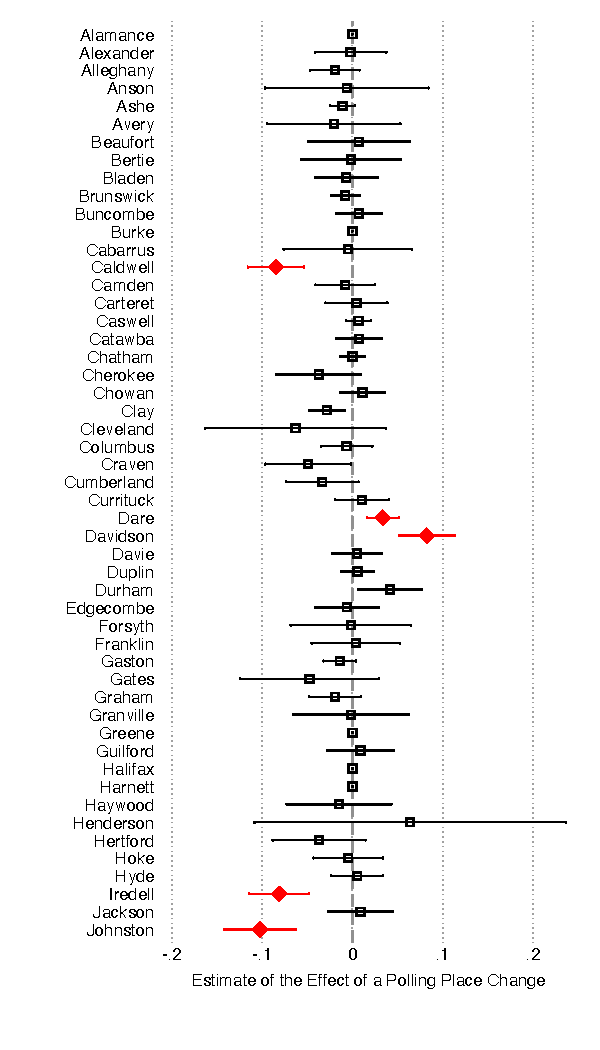
\includegraphics[ width=3in,  clip=true,  trim= 0.0in 0in 0in 0in ]{../../50_results_full/Plot_County_Coefficients_elecvote1.pdf}
		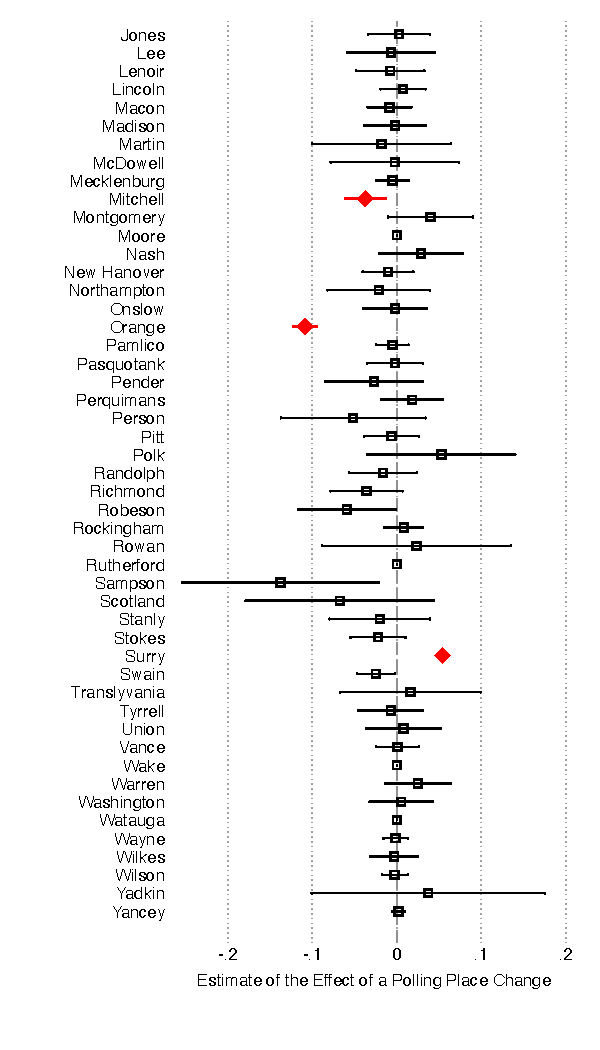
\includegraphics[ width=3in,  clip=true,  trim= 0.0in 0in 0in 0in ]{../../50_results_full/Plot_County_Coefficients_elecvote2.pdf}
		\label{county_elec_appendix}
		\end{center}
	\scriptsize{\emph{Notes:}   The above plot presents estimates of Equation~\ref{equation_traveltime_panel} for each county individually along with 95\% confidence intervals.  The outcome is $Pr(VoteElecDay)$.   Statistically insignificant estimates are presented with a black dot, those estimates statistically different from zero are presented with a hollow diamond.  Some county estimates cannot be estimated because no precincts in those counties experienced a polling place change. }
\end{figure} \normalsize

Given that the existing literature has estimated effects for counties alone, we present these county-specific estimates to highlight the fact that there is substantial heterogeneity in the effect across counties.  For example, in the case of Election Day voting, we can recover estimates of the effect of a polling place change that are both positive, negative and indistinguishable from zero (with varying degrees of precision).  Recall that we use a 10\% sample of from our sample of voters to estimate our effects for computational reasons.  This increases the imprecision of our estimates, but \emph{not} the coefficient estimate itself.








%% FIGURE: County plots of the effect of polling place change on early voting turnout
%%-------------------------------------------------------------------------------------------------------------
\begin{figure}[h!]
	\begin{center}
	\caption{County-Specific Estimates of the Effect of a Polling Place Change on Early Voting}
		\small \vspace*{.05in}
		\smallskip
		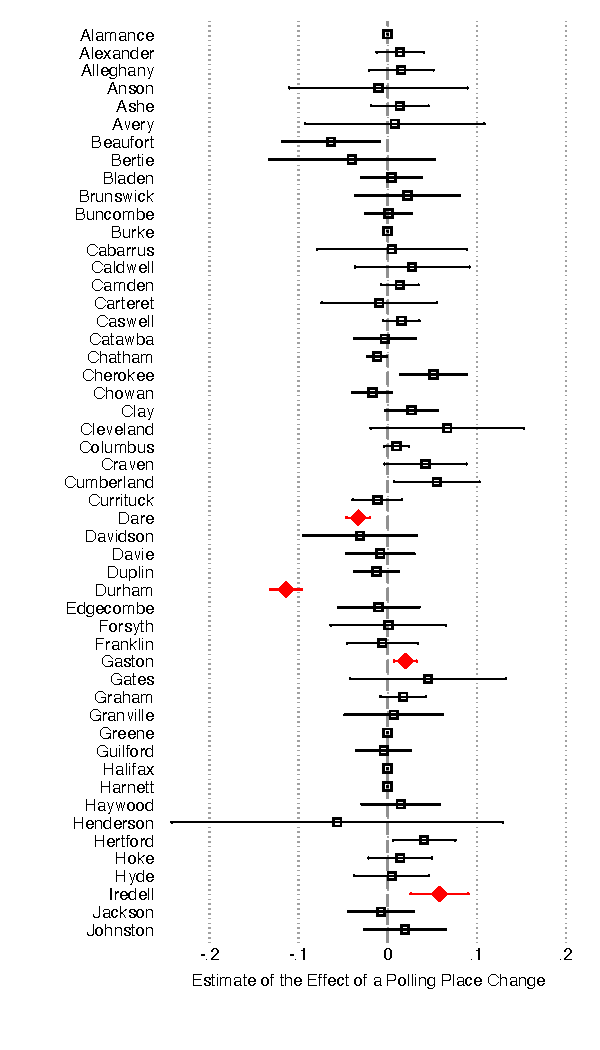
\includegraphics[ width=3in,  clip=true,  trim= 0.0in 0in 0in 0in ]{../../50_results_full/Plot_County_Coefficients_earlyvote1.pdf}
		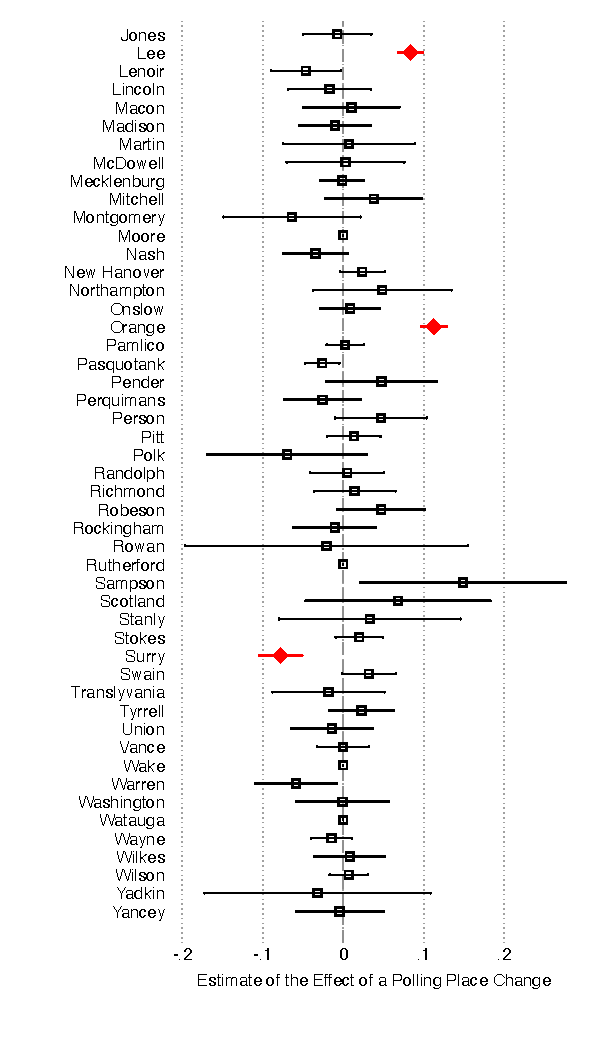
\includegraphics[ width=3in,  clip=true,  trim= 0.0in 0in 0in 0in ]{../../50_results_full/Plot_County_Coefficients_earlyvote2.pdf}
		\label{county_early_appendix}
		\end{center}
	\scriptsize{\emph{Notes:}   The above plot presents estimates of Equation~\ref{equation_traveltime_panel} for each county individually along with 95\% confidence intervals.  The outcome is $Pr(VoteEarly)$.   Statistically insignificant estimates are presented with a black dot, those estimates statistically different from zero are presented with a hollow diamond. Some county estimates cannot be estimated because no precincts in those counties experienced a polling place change.  }
\end{figure} \normalsize


The fact that there is variation across counties highlights the importance of our statewide estimates for understanding how polling place location changes affect statewide contests.  These results suggest that results from a single county \emph{cannot} be generalized to the state level, and doing so would likely lead to deeply erroneous conclusions.

That there is variation in the estimates is quite interesting, however we note that the purpose of our paper is not to theorize and test why the effects of polling place changes differ by counties (although we note that our results in the main paper suggest that it is \emph{not} a function of differences in the availability of early voting hours and locations).  Our purpose is to estimate the effect of polling place changes across an entire state (and to do so more rigorously and precisely than even county-level estimates have previously been estimated).  Of note is that the distribution of the estimates follows a normal distribution as indicated by Figure~\ref{county_distribution}, which suggests that variation may be due to voter-level shocks rather than systematic county-level differences.




%% FIGURE: County distribution of polling place changes
%%-----------------------------------------------------
\begin{figure}[h!]
	\begin{center}
	\caption{Distribution of the County-Specific Estimates of the Effect of a Polling Place Change on Overall Voter Turnout}
		\small \vspace*{.05in}
		\smallskip
		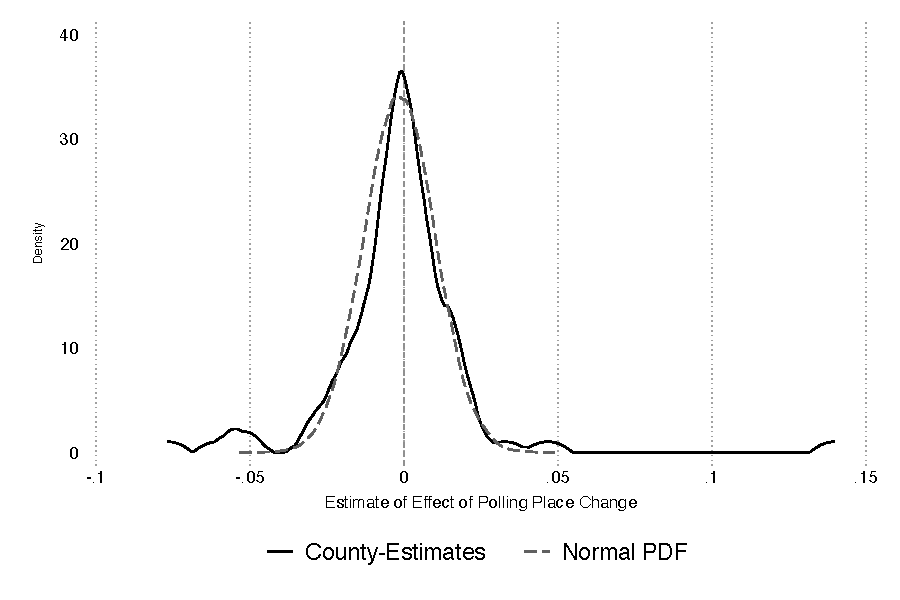
\includegraphics[ width=3.8in,  clip=true,  trim= 0.0in 0in 0in 0in ]{../../50_results_full/nc1_county_point_estimate_density_any.pdf}
		\label{county_distribution}
		\end{center}
	\scriptsize{\emph{Notes:}  The above plot presents estimates of Equation~\ref{equation_traveltime_panel} for each county individually along with 95\% confidence intervals.  The outcome is $Pr(VoteAny)$.  }
\end{figure} \normalsize









%------------------------------------ Appendix F: Substitution versus composition -------------------------------------%
\clearpage \newpage
\subsection{G. Substitution versus Composition}\label{appendix_substitution_v_composition}
\setcounter{table}{0}
\setcounter{figure}{0}
\renewcommand{\thetable}{G\arabic{table}}
\renewcommand{\thefigure}{G\arabic{figure}}

\noindent In order to establish whether the decline in Election Day voting and rise in early voting is the result of \emph{substitution} of Election Day voters into early voting or alternatively a decline in Election Day voting by one group of individuals and a rise in early voting \emph{by a different} group of previous non-voters, we examine two empirical patterns.

First, we estimate whether the effect of a polling place change on voting early varies by whether the voter voted on Election Day in the previous presidential election. Vote history can be thought of as a proxy for vote intention (absent a polling place change), and so if polling place changes are driving substitution into early voting by voters \emph{who would otherwise vote on Election Day}, we should see a \emph{larger} effect of polling place changes on early voting within this population. As shown in Table~\ref{table_pp_panel_lagged_interaction}, this is precisely what we observe -- voters who voted on Election Day in the last election and are impacted by a polling place change are almost 150\% more likely to vote early than other voters who experience a polling place change.



% TABLE 4: Average Effect of Polling Place Changes
%-------------------------------------------------
\begin{table}[h!]\centering \scriptsize
\def\sym#1{\ifmmode^{#1}\else\(^{#1}\)\fi}
	\caption{The Differential Effect of Polling Place Changes on Voter Turnout by Past Voting Mode}\label{table_pp_panel_lagged_interaction}
	\smallskip
	\begin{tabular}{@{\extracolsep{5pt}}l*{4}{c}}
	\noalign{\smallskip}\hline\hline\noalign{\smallskip}\noalign{\smallskip}
			&  \multicolumn{1}{c}{$Pr(VoteElecDay)$} &  \multicolumn{1}{c}{$Pr(VoteEarly)$} &  \multicolumn{1}{c}{$Pr(VoteAny)$}  \\
			\cline{2-4}  \noalign{\smallskip}
				                &\multicolumn{1}{c}{(1)}         &\multicolumn{1}{c}{(2)}         &\multicolumn{1}{c}{(3)}         \\
\midrule
$\Delta$\emph{PollingPlace} $(\hat{\beta})$&   -0.011\sym{***}&    0.012\sym{***}&  0.00034         \\
                & (0.0023)         & (0.0027)         & (0.0018)         \\
\emph{LagElecDayVoter}$\cdot \Delta PollingPlace$&   -0.032\sym{***}&    0.025\sym{***}&  -0.0053\sym{**} \\
                & (0.0034)         & (0.0035)         & (0.0022)         \\
\midrule
Individual FE   &                  &                  &                  \\
Indiv. Controls &\checkmark         &\checkmark         &\checkmark         \\
Year FE         &\checkmark         &\checkmark         &\checkmark         \\
County x Year FE&\checkmark         &\checkmark         &\checkmark         \\
Race x Year FE  &\checkmark         &\checkmark         &\checkmark         \\
Year Sample     &Full Panel         &Full Panel         &Full Panel         \\
Observations    &  4680586         &  4680586         &  4680586         \\
Mean of DV      &     0.30         &     0.46         &     0.80         \\
SD of DV        &     0.45         &     0.49         &     0.40         \\
 \\
	\noalign{\vspace*{-.10in}}\hline\hline\noalign{\smallskip}
\multicolumn{4}{p{4.3in}}{\scriptsize Standard errors clustered by precinct assignment history. } \\
\multicolumn{4}{l}{\scriptsize \sym{*} \(p<0.1\), \sym{**} \(p<0.05\), \sym{***} \(p<0.01\)}\\
\multicolumn{4}{p{4.3in}}{\scriptsize  \emph{Notes}: The table presents coefficients from estimating a version of Equation~\ref{equation_traveltime_panel} with no travel time coefficients, no fixed effects, and demographic controls from Equation~\ref{equation_aggregate_crosssectional_closefurther}. Omission of individual fixed effects is necessary as use of lagged dependent variables in a short panel results in Nickell bias \citep{Nickell:1981eo}. The unit of analysis is the voter-election.   }
\end{tabular}
\end{table}



As an additional test, we examine whether the \emph{composition} of voters varies between precincts with polling place changes and precincts without polling place changes.  If mailers are inducing what would otherwise be non-voters to vote, and preventing election-day voters from voting, then we would expect the overall composition of voters who cast a ballot to change as well.

Table \ref{table_substitution_v_composition} correlates overall turnout with voter party and polling place change. Note that these estimations exclude individual fixed effects, which is necessary when including lagged dependent variables in a short panel to avoid Nickell bias.  In general, the results tend to support the idea of substitution --- while there is some change in the composition of the electorate, the estimates are inconsistent across specifications and small in comparison to the degree of substitution observed --- about one-half percentage point change in composition versus    -0.7 and     0.6 percentage point changes in Election Day and early voting respectively. Combined with the fact that the largest effects of a polling place change occur among those who previously voted on Election Day -- a reasonable proxy for vote intention absent a polling place change --- it seems reasonable to conclude that the offsetting effects that we identify are a consequence of voters reacting to a change in polling place location by voting early rather than staying home.


% TABLE X: Polling Place Changes and Voter Composition
%------------------------------------------------------
\begin{table}[t!]\centering \scriptsize
\def\sym#1{\ifmmode^{#1}\else\(^{#1}\)\fi}
	\caption{Polling Place Changes and Voter Composition}\label{table_substitution_v_composition}
	\smallskip
	\begin{tabular}{@{\extracolsep{5pt}}l*{4}{c}}
	\noalign{\smallskip}\hline\hline\noalign{\smallskip}\noalign{\smallskip}
			&  \multicolumn{1}{c}{$Pr(VoteAny)$} &  \multicolumn{1}{c}{$Pr(VoteAny)$} &  \multicolumn{1}{c}{$Pr(VoteAny)$}  \\
			\cline{2-4}  \noalign{\smallskip}
				                &\multicolumn{1}{c}{(1)}         &\multicolumn{1}{c}{(2)}         &\multicolumn{1}{c}{(3)}         \\
\midrule
$\Delta$\emph{PollingPlace} $(\hat{\beta})$&  -0.0033         &   0.0032         &  -0.0066\sym{***}\\
                & (0.0020)         & (0.0026)         & (0.0020)         \\
$\Delta$\emph{PollingPlace}$\cdot$\emph{Rep}&   0.0022         &  -0.0026         &   0.0042         \\
                & (0.0026)         & (0.0025)         & (0.0028)         \\
$\Delta$\emph{PollingPlace}$\cdot$\emph{Unaffil}&   0.0048         &  -0.0017         &   0.0065\sym{**} \\
                & (0.0032)         & (0.0020)         & (0.0026)         \\
\midrule
Individual FE   &\checkmark         &                  &                  \\
Year FE         &\checkmark         &                  &                  \\
County x Year FE&\checkmark         &                  &                  \\
Race x Year FE  &\checkmark         &                  &                  \\
County FE       &                  &\checkmark         &\checkmark         \\
Controls        &                  &\checkmark         &\checkmark         \\
Year Sample     &Full Panel         &     2012         &     2016         \\
Observations    &  4677529         &  2338392         &  2337937         \\
Mean of DV      &     0.80         &     0.84         &     0.75         \\
SD of DV        &     0.21         &     0.36         &     0.43         \\
Party Joint Sig &     0.32         &     0.50         &    0.050         \\
 \\
	\noalign{\vspace*{-.17in}}\hline\hline\noalign{\smallskip}
\multicolumn{4}{p{4.3in}}{\scriptsize Standard errors clustered by precinct assignment history. } \\
\multicolumn{4}{l}{\scriptsize \sym{*} \(p<0.1\), \sym{**} \(p<0.05\), \sym{***} \(p<0.01\)}\\
\multicolumn{4}{p{4.3in}}{\scriptsize  \emph{Notes}: Omitted party ID is Democrat. A very small quantity of libertarians have been excluded for ease of interpretation. The table presents coefficients from estimating Equation~\ref{equation_traveltime_panel} without travel time coefficients.  The unit of analysis is the voter-election. The SD of the DV in the panel is the average of the within-$i$ standard deviations of the outcome variable. }
\end{tabular}
\end{table}











%---------------------------------- APPENDIX H: TRAVEL TIME -------------------------------------%
\clearpage \newpage
\subsection{H. Additional Plots for Travel Time Changes}\label{appendix_distributionppchanges}
\setcounter{table}{0}
\setcounter{figure}{0}
\renewcommand{\thetable}{H\arabic{table}}
\renewcommand{\thefigure}{H\arabic{figure}}


\noindent In the main paper, we pool the distributions of polling place distance changes and changes in drive time across our period.  In this appendix, we present the distributions separately for each year.  The separate distributions reveal little difference in either measure across years with the following exception --- in 2016, there were fewer people moved \emph{significantly} closer ($>10$ minutes) closer to their polling place (lower right plot).  But the number of individuals in the tail of the distribution there is extremely small.



%% FIGURE: Distribution Drive Time By Year, Appendix
%%--------------------------------------------------
\begin{figure}[h!]
	\begin{center}
	\caption{Distribution of Distance of Polling Place Changes and Changes in Drive Time by Year}
		\small \vspace*{.05in}
		\bigskip
		Change in Distance Between Past  and Current Polling Place Location \\
		\smallskip
		2012   \hspace*{2.85in} 2016 \\
		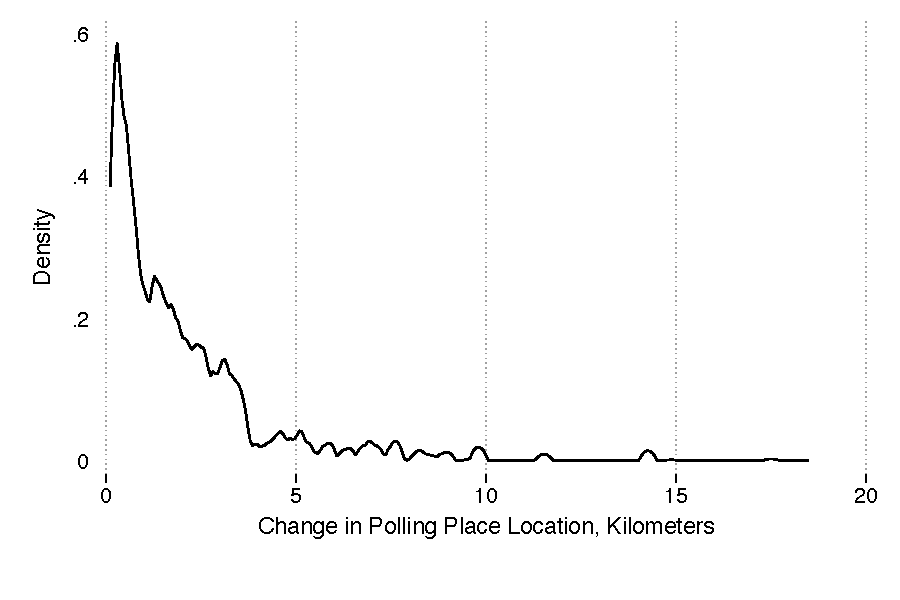
\includegraphics[ width=3in,  clip=true,  trim= 0.0in 0in 0in 0in ]{../../50_results_full/Plot_Distribution_PPMoveDistance_2012.pdf}
		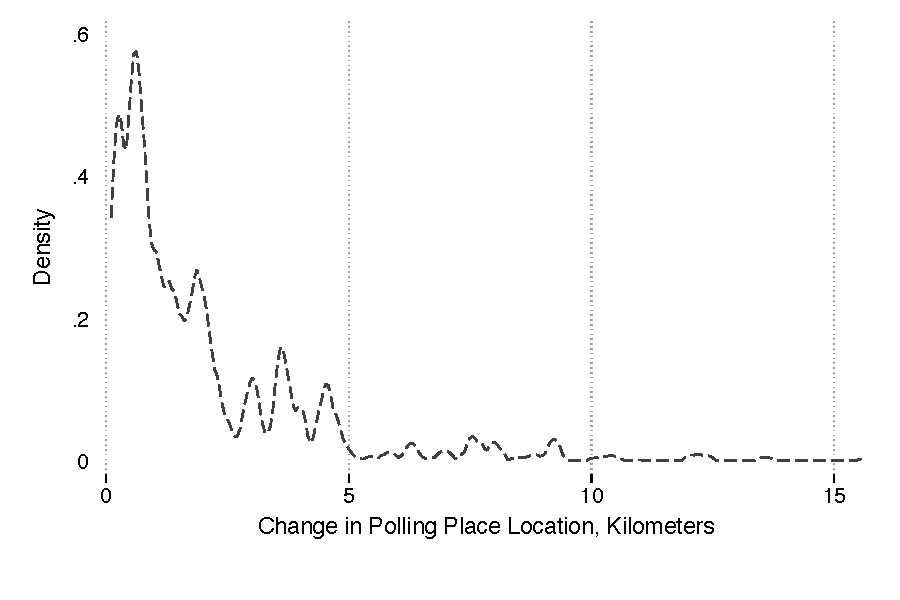
\includegraphics[ width=3in,  clip=true,  trim= 0.0in 0in 0in 0in ]{../../50_results_full/Plot_Distribution_PPMoveDistance_2016.pdf} \\

		Change in Drive Time to Polling Place and Current Polling Place Location \\
		\smallskip
		2012   \hspace*{2.85in} 2016 \\
		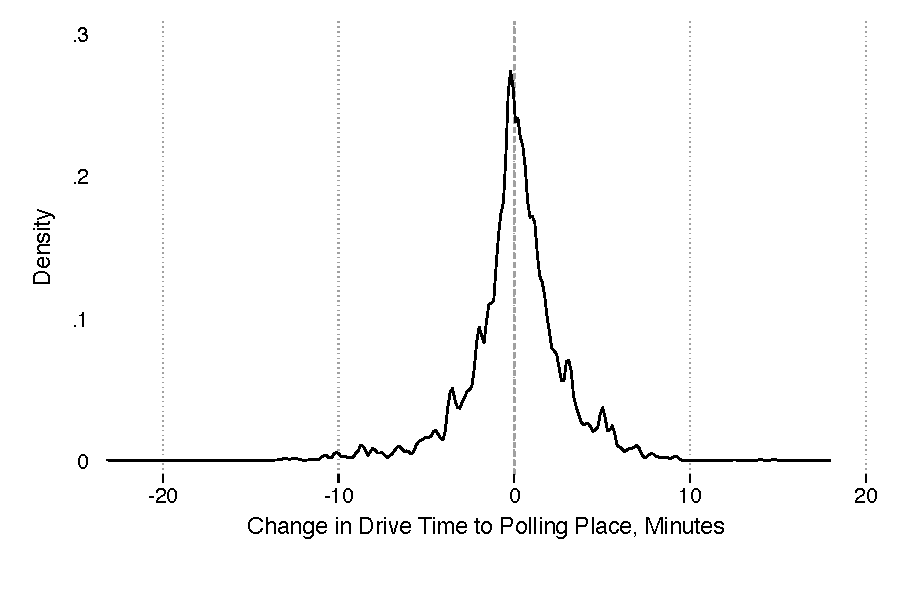
\includegraphics[ width=3in,  clip=true,  trim= 0.0in 0in 0in 0in ]{../../50_results_full/Plot_Distribution_DriveTime_2012.pdf}
		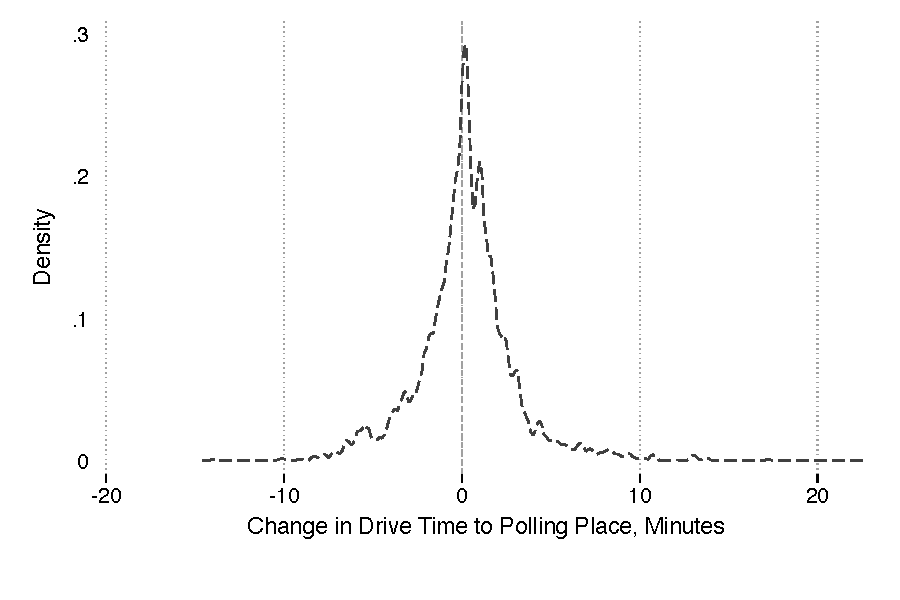
\includegraphics[ width=3in,  clip=true,  trim= 0.0in 0in 0in 0in ]{../../50_results_full/Plot_Distribution_DriveTime_2016.pdf}
		\label{figure_traveltime_distribution_appendix}
		\end{center}
	\scriptsize{\emph{Notes:}  The upper two presents the distribution of the distance between a precinct's polling place location in a given election year relative to its location in the previous election year, conditional on a voters' polling place having moved.  The unit of analysis in plot (a) is a voter; therefore, distance changes are weighted by the number of voters experiencing the change.  Polling place changes can result from the movement of a given individual's polling place, or from a voter being moved into a new precinct by a precinct boundary change.  Plot (b) presents the distribution of changes in drive time to a polling place for voters who experienced a polling place change.  Note that some voters can experience a polling place change without a change in drive time. }
\end{figure} \normalsize




%  FIGURE: Scatterplots of Drive Time and Total Voter Turnout
%---------------------------------------------------------------------------------
\begin{figure}[t!]
	\begin{center}
	\caption{Relationship Between the Change in Driving Time to Polling Place and Overall Turnout}
		\small \vspace*{.05in}
		\smallskip
				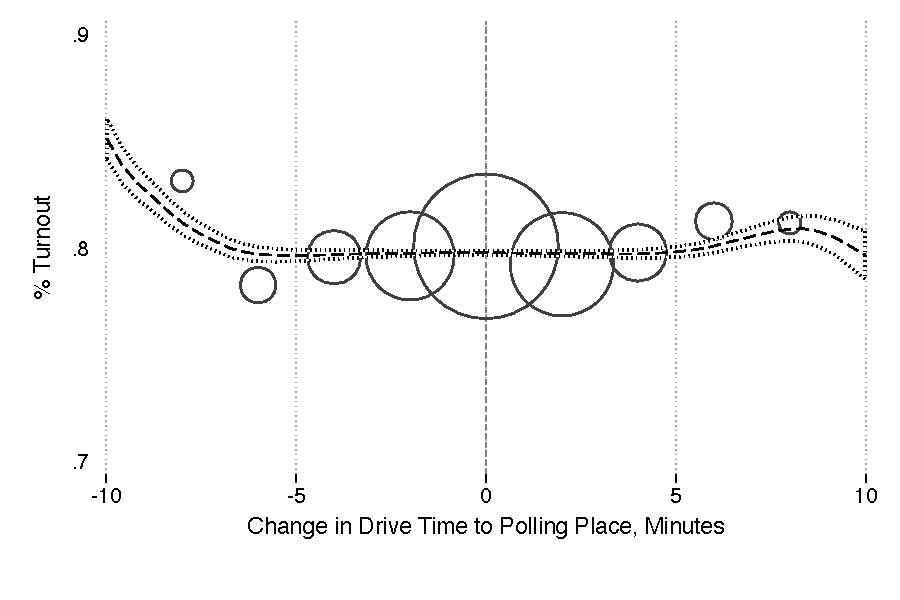
\includegraphics[ width=3.35in,  clip=true,  trim= 0.0in 0in 0in 0in ]{../../50_results_full/Plot_Scatter_DriveTime_ANY.pdf}
		\label{figure_scatter_drivetime_appendix}
		\end{center}
	\scriptsize{\emph{Notes:}   The above scatter plot presents the bivariate relationship between the change in drive time to polling place (measured in minutes) from the previous presidential election year and total voter turnout.  Change in drive time is conditional on a voter not having moved and having had their polling place change.  Hollow circles are binned averages of the outcome for every 2 minute interval of drive time change.  The circles are sized relative to the population in the bin.  We do not plot the very few observations at the tails of the distribution (those with drive time changes that are greater than 1.5 times the 99th percentile of drive time changes).  The dashed line represents a local polynomial fit (bandwidth = 3).  The fit lines are fit to all of the data, not just the bins.  However, we restrict the fits to within 10 minutes since the confidence intervals in the tails are extremely large as a consequence of the limited number of observations with large drive time changes.  Circles to the left of the vertical line at zero represent voters who had a polling place moved \emph{closer} to them; circles to the right of the vertical line at zero represent voters who had a polling place moved \emph{farther} away.  Data is pooled across 2012 and 2016.}
\end{figure} \normalsize







%--------------------------------------- APPENDIX I:  AGE ----------------------------------%
\clearpage \newpage
\subsection{I. Differential Effects by Age}\label{appendix_age}
\setcounter{table}{0}
\setcounter{figure}{0}
\renewcommand{\thetable}{I\arabic{table}}
\renewcommand{\thefigure}{I\arabic{figure}}


\noindent In this appendix, we examine whether the effects that we estimate in the main paper depend on the age of voters.

The expected effects of age on polling place changes are uncertain.  If older voters have a longer habit of voting a specific way --- e.g., at a specific Election Day polling place --- then they may be more impacted by a change in the location of their polling place relative to a younger voter with weaker voting habits tied to a particular polling place or mode.  However, if older voters have a stronger habit of voting \emph{generally} regardless of mode, polling place changes may be \emph{less} impactful because of their increased motivation to overcome the costs of polling place changes, or because they do not require a prime to remember to vote.  The youngest voters may also have higher expectations of costs associated with voting (precisely because they have not developed a habit of voting by a particular mode or at all), making a polling place change less disruptive because it is already factored into expectations.

Age-related differences may also impact the relative importance of priming, search costs and travel costs in uncertain ways.  Younger voters may be more attuned to technology and better able to locate new polling places than older voters, but they may also be better able to locate early voting locations when informed of a change in their polling place location by an official notification.  The willingness to risk a new polling place on Election Day rather than vote early may also vary by age if employed individuals are more likely to vote early than try to find a new polling place on Election Day.




%  FIGURE: Scatterplots of Age and Type of Voting
%------------------------------------------------
\begin{figure}[h!]
	\begin{center}
	\caption{Relationship Between Age, Mode of Voting and Polling Place Change}
		\small \vspace*{.05in}
		\smallskip
		\hspace*{.1in} (a) Election Day Voting  \hspace*{1.8in} (b) Early Voting \\
				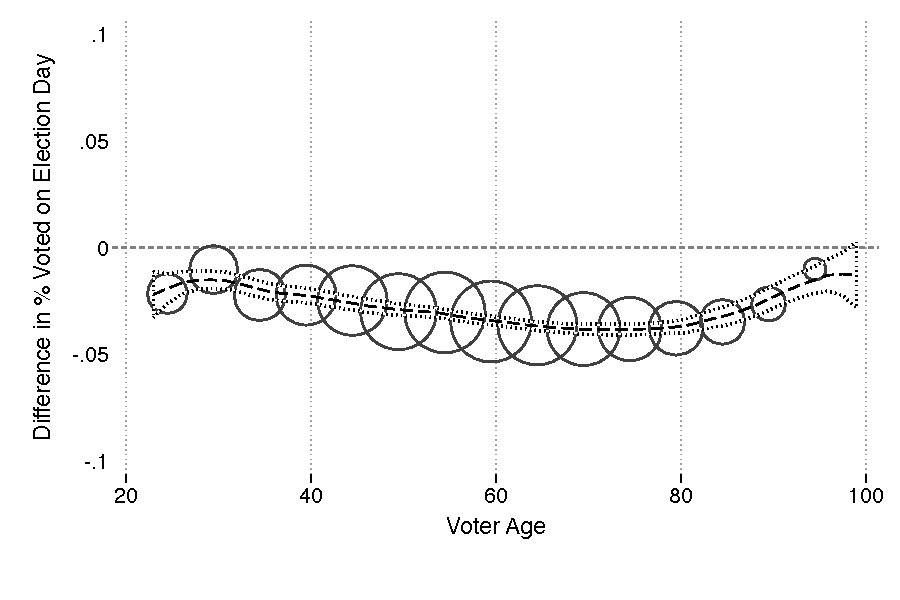
\includegraphics[ width=3in,  clip=true,  trim= 0.0in 0in 0in 0in ]{../../50_results_full/Plot_Scatter_Age_elecday_ppchange.pdf}
				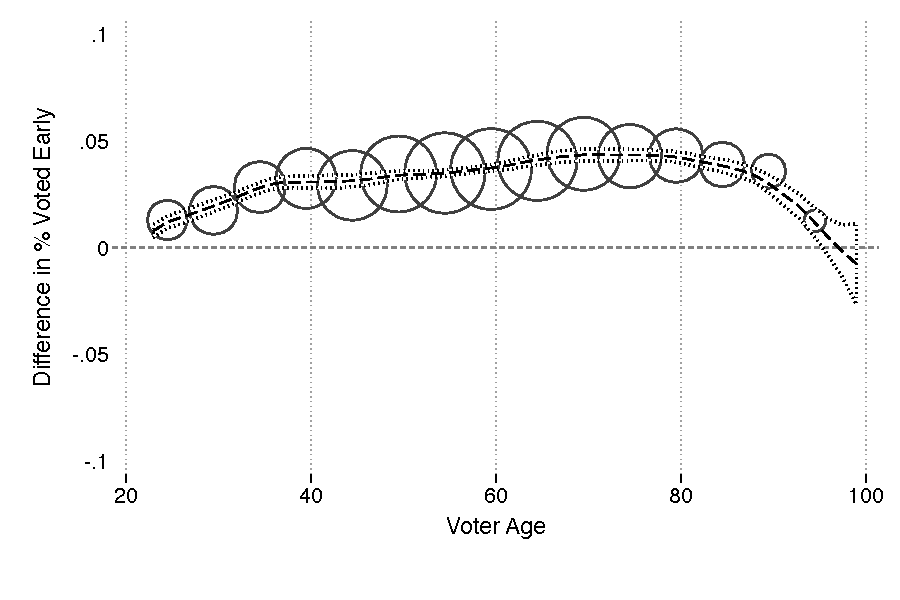
\includegraphics[ width=3in,  clip=true,  trim= 0.0in 0in 0in 0in ]{../../50_results_full/Plot_Scatter_Age_early_ppchange.pdf} \\
		\label{figure_scatter_age}
		\end{center}
	\scriptsize{\emph{Notes:}   The graphs present the relationship between age (in 2016) and the difference in turnout between those who do and do not experience a polling place change for Election Day voting (a) and early voting (b).  The hollow circles are sized relative to the population in the bin (at 5 year intervals).  The dashed line represents a local polynominal (bandwidth = 3) fit to all of the data, not just the bins, pooled across 2012 and 2016.  The gray horizontal line denotes no difference in turnout -- circles above (below) zero represent instances of higher (lower) turnout amongst those who experience a polling place change relative to those who do not.}
\end{figure} \normalsize

Figure~\ref{figure_scatter_age} plots the difference in voting behavior by age in 2016 for those who did and did not experience a change in polling place.   Voters are binned into 5 year age bins where the size of the bins corresponds to the sample size.  Points above (below) zero indicate instances when voters of a given age turnout more on average when they experience a polling place relative to those who do not.

The plots in Figure~\ref{figure_scatter_age} provide some evidence that the substitution into early voting in response to a polling place change varies by age.  In particular, the youngest and oldest voters have the smallest declines in Election Day voting and the smallest increases in early voting --- indicating that polling place changes are less likely to affect how they vote relative to middle-aged voters affected by a polling place change.  Voters in the middle of the distribution --- voters who are also most likely to be employed and invested in the community --- are the voters who are most likely to substitute to early voting in response to a polling place change. That said, the net effects of these two effects completely offset and overall turnout does not vary by age in response to a polling place change (figure~\ref{figure_scatter_age_any}).

% I don't know what this means:  That overall turnout does not change but middle-aged individuals are slightly more likely to substitute into early voting in response to a change in polling place location than younger or older voters suggests, but certainly does not prove, that different mechanisms may be responsible for the effects.

The fact that the youngest voters are the least likely to substitute into early voting suggests that they may be the most responsive to the informational mailers that remind them of their new polling place.  They may also better able to overcome the search and confusion costs associated with finding a new polling place given technological changes (e.g., smartphones).  Although the information mailers lack the emotional appeals found in much of the GOTV literature in political science \citep{gerber2017generalizability, gerber2008social}, the information provided may be sufficiently informative and the election competitive enough that the mailer is enough to mobilize younger voters who are less likely generally to participate \citep{arceneaux2009mobilized}.  Middle-aged voters may fear the uncertainty of a change in polling place location -- especially if they are motivated to vote in the high-stakes competitive presidential election contest -- and they may choose to vote early rather that risk the consequences of trying to cast an Election Day vote at a new polling place.  Although our investigations are not well-positioned to identify the particular mechanisms responsible for the substitution patterns we characterize, our results do suggest that age (or age-correlated characteristics) has only a limited impact of the effects of polling place changes.



%In this appendix, we present additional results related to the effects of polling place changes and drive times by age.  First, in Figure~\ref{figure_scatter_age_any} we show a scatterplot like those presented in the main paper for overall turnout.  Consistent with the results for early and Election Day voting in the paper, there are few differences in effects for age across the majority of the distribution.  However, those youngest voters in our sample are more likely to turnout to vote when their polling place has changed relative to voters of the same age who do not.  Although perhaps surprising, we think that this is likely a function of the mailer that voters receive when their polling place has changed.  This likely serves as a reminder to younger voters to turnout who have not yet developed a habit of voting.




%  FIGURE: Scatterplots of Age and Type of Voting
%------------------------------------------------
\begin{figure}[h!]
	\begin{center}
	\caption{Relationship Between Age, Overall Turnout and Polling Place Change}
		\small \vspace*{.05in}
				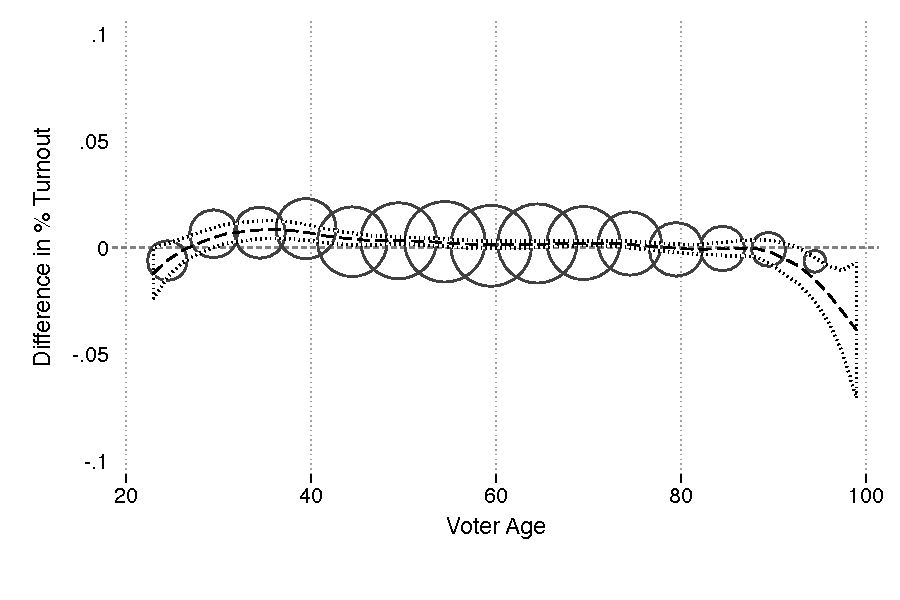
\includegraphics[ width=3.35in,  clip=true,  trim= 0.0in 0in 0in 0in ]{../../50_results_full/Plot_Scatter_Age_any_ppchange.pdf}
		\label{figure_scatter_age_any}
		\end{center}
	\scriptsize{\emph{Notes:}   The above scatter plot presents the simple bivariate relationship between age and the difference in turnout between those who experience a polling place change and those who do not for all modes of voting (overall turnout).  The hollow circles are sized relative to the population in the bin (at 5 year intervals).  The dashed line represents a local polynominal fit (bandwidth = 3).  The fit lines are fit to all of the data, not just the bins.  Data is pooled across 2012 and 2016.  The gray horizontal line is at zero; no difference in turnout.  Circles above zero represent instances of higher turnout amongst those who experience a polling place change relative to those who do not, while circles below zero represent instances of lower turnout amongst those who experience a polling place change relative to those who do not.}
\end{figure} \normalsize


The distribution of ages in our sample of voters is presented in Figure~\ref{figure_density_age_any}.


To more formally investigate the relationship between age, polling place change and voter turnout, we estimate the specifications from the main paper.  We trichotomize age to make it easier to interpret differential effects.  In particular, we construct an $Age <26$ category (dummy) for the youngest voters in our sample, and an $Age>76$ category (dummy) for the oldest voters in our sample.  These categorical variables allow us to estimate intercept shifts for the group, but constrain the slope of the effect by age.  The residual, or base category, is for voters between 26 and 76.




%  FIGURE:  Density Age
%----------------------
\begin{figure}[h!]
	\begin{center}
	\caption{Distribution of Age}
		\small \vspace*{.05in}
				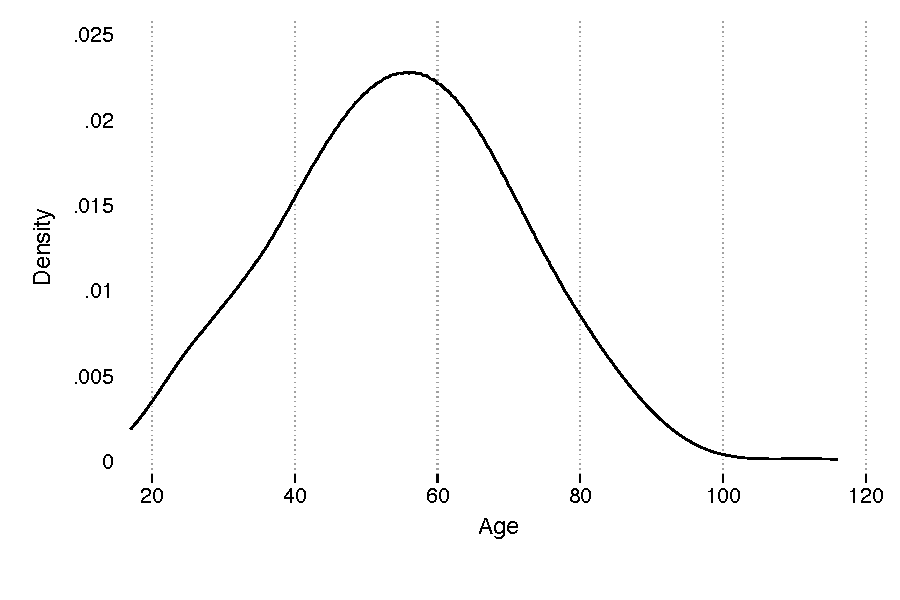
\includegraphics[ width=3.35in,  clip=true,  trim= 0.0in 0in 0in 0in ]{../../50_results_full/Plot_Distribution_Age.pdf}
		\label{figure_density_age_any}
		\end{center}
	\scriptsize{\emph{Notes:}   The above plot is the distribution of voter age in our sample for all years.}
\end{figure} \normalsize


%We might expect that the youngest voters, who have less of a habit of voting, would be less likely to turnout when their polling place has changed.  The oldest voters, who have potentially the longest habit of voting would be more likely to overcome costs and turnout.  Although we note that a polling place change might be more psychologically costly if you have developed a long habit of voting in a particular place and result in a decline in turnout.  Although the literature generally finds higher turnout among older voters who have more time and may value voting more, we also note that older voters may also be less resourced and less able to substitute or overcome polling place change costs.




% TABLE: Heterogeneity in Age, Panel
%------------------------------------
\begin{table}[h!]\centering \scriptsize
\def\sym#1{\ifmmode^{#1}\else\(^{#1}\)\fi}
	\caption{The Differential Effect of Polling Place Changes on Voter Turnout by Age}\label{table_pp_panel_age}
	\smallskip
	\begin{tabular}{@{\extracolsep{5pt}}l*{4}{c}}
	\noalign{\smallskip}\hline\hline\noalign{\smallskip}\noalign{\smallskip}
			&  \multicolumn{1}{c}{$Pr(VoteElecDay)$} &  \multicolumn{1}{c}{$Pr(VoteEarly)$} &  \multicolumn{1}{c}{$Pr(VoteAny)$}  \\
			\cline{2-4}  \noalign{\smallskip}
				                &\multicolumn{1}{c}{(1)}         &\multicolumn{1}{c}{(2)}         &\multicolumn{1}{c}{(3)}         \\
\midrule
$\Delta$\emph{PollingPlace} $(\hat{\beta})$&  -0.0065\sym{*}  &   0.0055         &  -0.0018         \\
                & (0.0039)         & (0.0048)         & (0.0026)         \\
$\Delta PollingPlace \cdot$\emph{Age <26}&   0.0017         &  -0.0054         &  -0.0017         \\
                & (0.0097)         & (0.0098)         &  (0.011)         \\
$\Delta PollingPlace \cdot$\emph{Age 76+}&  -0.0049         &   0.0059         &   0.0018         \\
                & (0.0056)         &  (0.016)         &  (0.014)         \\
\midrule
Individual FE   &\checkmark         &\checkmark         &\checkmark         \\
Year FE         &\checkmark         &\checkmark         &\checkmark         \\
County x Year FE&\checkmark         &\checkmark         &\checkmark         \\
Race x Year FE  &\checkmark         &\checkmark         &\checkmark         \\
Year Sample     &Full Panel         &Full Panel         &Full Panel         \\
Observations    &  4681792         &  4681792         &  4681792         \\
Mean of DV      &     0.30         &     0.46         &     0.80         \\
SD of DV        &     0.25         &     0.26         &     0.21         \\
 \\
	\noalign{\vspace*{-.10in}}\hline\hline\noalign{\smallskip}
\multicolumn{4}{p{4.0in}}{\scriptsize Standard errors clustered by precinct assignment history. } \\
\multicolumn{4}{l}{\scriptsize \sym{*} \(p<0.1\), \sym{**} \(p<0.05\), \sym{***} \(p<0.01\)}\\
\multicolumn{4}{p{4.0in}}{\scriptsize  \emph{Notes}: The table presents coefficients from estimating Equation~\ref{equation_traveltime_panel} without the travel time indicators but with the addition of age dummies. The unit of analysis is the voter-election.  The SD of the DV is the average of the within-$i$ standard deviations of the outcome. }
\end{tabular}
\end{table}





% TABLE: Polling Place Changes and Travel Costs by Mode of Voting and Age
%------------------------------------------------------------------------
\begin{table}[h!]\centering \scriptsize
\def\sym#1{\ifmmode^{#1}\else\(^{#1}\)\fi}
	\caption{The Differential Effect of Changes in Travel Time to Polling Place on Turnout by Age}\label{table_pp_panel_closefurther_age}
	\smallskip
	\begin{tabular}{@{\extracolsep{5pt}}l*{4}{c}}
	\noalign{\smallskip}\hline\hline\noalign{\smallskip}\noalign{\smallskip}
			&  \multicolumn{1}{c}{$Pr(VoteElecDay)$} &  \multicolumn{1}{c}{$Pr(VoteEarly)$} &  \multicolumn{1}{c}{$Pr(VoteAny)$}  \\
			\cline{2-4}  \noalign{\smallskip}
				                &\multicolumn{1}{c}{(1)}         &\multicolumn{1}{c}{(2)}         &\multicolumn{1}{c}{(3)}         \\
\midrule
$\Delta$\emph{PollingPlace} $(\hat{\beta})$&  -0.0065\sym{*}  &   0.0055         &  -0.0018         \\
                & (0.0039)         & (0.0048)         & (0.0026)         \\
$\Delta PollingPlace \cdot$\emph{Age <26}&   0.0041         &  -0.0045         & -0.00021         \\
                & (0.0100)         & (0.0100)         &  (0.011)         \\
$\Delta PollingPlace \cdot$\emph{Age 76+}&  -0.0034         &   0.0041         &  0.00085         \\
                & (0.0059)         &  (0.016)         &  (0.014)         \\
$\Delta MuchCloser \cdot$\emph{Age <26}&   -0.055         &    0.020         &  -0.0089         \\
                &  (0.041)         &  (0.039)         &  (0.048)         \\
$\Delta MuchCloser \cdot$\emph{Age <26}&   -0.032         &   -0.041         &   -0.038         \\
                &  (0.039)         &  (0.038)         &  (0.042)         \\
$\Delta MuchCloser \cdot$\emph{Age 76+}&   0.0015         &    0.016         &    0.024         \\
                &  (0.017)         &  (0.046)         &  (0.038)         \\
$\Delta MuchCloser \cdot$\emph{Age 76+}&   -0.040\sym{**} &    0.034         &   0.0041         \\
                &  (0.017)         &  (0.037)         &  (0.041)         \\
\midrule
Individual FE   &\checkmark         &\checkmark         &\checkmark         \\
Year FE         &\checkmark         &\checkmark         &\checkmark         \\
County x Year FE&\checkmark         &\checkmark         &\checkmark         \\
Race x Year FE  &\checkmark         &\checkmark         &\checkmark         \\
Year Sample     &Full Panel         &Full Panel         &Full Panel         \\
Observations    &  4681792         &  4681792         &  4681792         \\
Mean of DV      &     0.30         &     0.46         &     0.80         \\
SD of DV        &     0.25         &     0.26         &     0.21         \\
 \\
	\noalign{\vspace*{-.10in}}\hline\hline\noalign{\smallskip}
\multicolumn{4}{p{4.3in}}{\scriptsize Standard errors clustered by precinct assignment history. } \\
\multicolumn{4}{l}{\scriptsize \sym{*} \(p<0.1\), \sym{**} \(p<0.05\), \sym{***} \(p<0.01\)}\\
\multicolumn{4}{p{4.3in}}{\scriptsize  \emph{Notes}: The table presents coefficients from estimating Equation~\ref{equation_traveltime_panel} with the addition of age dummies. The unit of analysis is the voter-election. The SD of the DV is the average of the within-$i$ standard deviations of the outcome.  }
\end{tabular}
\end{table}


Table~\ref{table_pp_panel_age} suggests no differential effects across any of our three outcome variables by age.  Similarly, when we examine differential effects in drive time in our panel in Table~\ref{table_pp_crosssec_age} none of the interactions are statistically significant.


% TABLE: Polling Place Changes by Mode of Voting, Cross-Sectional by Age
%------------------------------------------------------------------------
\begin{table}[h!]\centering \scriptsize
\def\sym#1{\ifmmode^{#1}\else\(^{#1}\)\fi}
	\caption{The Differential Effect of Polling Place Changes by Year by Age}\label{table_pp_crosssec_age}
	\smallskip
	\begin{tabular}{@{\extracolsep{5pt}}l*{6}{c}}
	\noalign{\smallskip}\hline\hline\noalign{\smallskip}\noalign{\smallskip}
			&  \multicolumn{2}{c}{$Pr(VoteElecDay)$} &  \multicolumn{2}{c}{$Pr(VoteEarly)$} &  \multicolumn{2}{c}{$Pr(VoteAny)$}  \\
			\cline{2-3} \cline{4-5} \cline{6-7} \noalign{\smallskip}
				                &\multicolumn{1}{c}{(1)}         &\multicolumn{1}{c}{(2)}         &\multicolumn{1}{c}{(3)}         &\multicolumn{1}{c}{(4)}         &\multicolumn{1}{c}{(5)}         &\multicolumn{1}{c}{(6)}         \\
\midrule
$\Delta$\emph{PollingPlace} $(\hat{\beta})$&   -0.016\sym{***}&   -0.029\sym{***}&    0.018\sym{***}&    0.025\sym{***}&   0.0025         &  -0.0027         \\
                & (0.0035)         & (0.0062)         & (0.0048)         & (0.0058)         & (0.0029)         & (0.0021)         \\
$\Delta PollingPlace \cdot$\emph{Age <26}& -0.00079         &    0.019\sym{**} &   -0.025\sym{**} &   -0.015\sym{*}  &   -0.017         &   0.0031         \\
                &  (0.013)         & (0.0073)         &  (0.012)         & (0.0077)         &  (0.020)         & (0.0099)         \\
$\Delta PollingPlace \cdot$\emph{Age 76+}&  -0.0036         &   0.0060         &    0.011\sym{***}&  -0.0090\sym{**} &   0.0031         &  -0.0052         \\
                & (0.0031)         & (0.0046)         & (0.0037)         & (0.0043)         & (0.0032)         & (0.0045)         \\
\emph{Age <26}  &   -0.091\sym{***}&   -0.030\sym{***}&    -0.19\sym{***}&    -0.15\sym{***}&    -0.26\sym{***}&    -0.17\sym{***}\\
                & (0.0042)         & (0.0033)         & (0.0098)         & (0.0033)         &  (0.011)         & (0.0039)         \\
\emph{Age 76+}  &   -0.053\sym{***}&   -0.028\sym{***}&    0.017\sym{***}&    -0.17\sym{***}&   0.0035         &    -0.19\sym{***}\\
                & (0.0030)         & (0.0050)         & (0.0021)         & (0.0046)         & (0.0032)         & (0.0043)         \\
\midrule
County FE       &\checkmark         &\checkmark         &\checkmark         &\checkmark         &\checkmark         &\checkmark         \\
Individual Controls&\checkmark         &\checkmark         &\checkmark         &\checkmark         &\checkmark         &\checkmark         \\
Year Sample     &     2012         &     2016         &     2012         &     2016         &     2012         &     2016         \\
Observations    &  2340293         &  2340293         &  2340293         &  2340293         &  2340293         &  2340293         \\
Mean of DV      &     0.33         &     0.26         &     0.47         &     0.45         &     0.84         &     0.75         \\
SD of DV        &     0.46         &     0.44         &     0.49         &     0.49         &     0.36         &     0.43         \\
 \\
	\noalign{\vspace*{-.10in}}\hline\hline\noalign{\smallskip}
\multicolumn{7}{p{5.2in}}{\scriptsize Robust standard errors in parentheses. } \\
\multicolumn{7}{l}{\scriptsize \sym{*} \(p<0.1\), \sym{**} \(p<0.05\), \sym{***} \(p<0.01\)}\\
\multicolumn{7}{p{5.2in}}{\scriptsize  \emph{Notes}: The table presents coefficients from estimating Equation~\ref{equation_aggregate_crosssectional_closefurther} without the travel time indicators and with the addition of age dummies.  The unit of analysis is the voter. The SD of the DV is the average of the within-county standard deviations of the outcome. }
\end{tabular}
\end{table}

When we turn to examining heterogeneity by age and by partisanship in our cross-sectional regressions there is some evidence that younger voters are differentially failing to show up at the polls in 2016 (as a consequence of Republican-controlled polling place changes), relative to 2012 when younger voters appear slightly more likely to turnout.  There are no consistent statistically significant effects for older voters.  Nor in Table~\ref{table_pp_crosssec_closerfurther_age} do we see consistent patterns that would indicate that voters of different ages responded differently to polling place changes in different years (i.e. under different partisan regimes).  Thus, consistent with our cross-sectional estimates for year in the main paper, we do find some evidence that Republican changes depressed turnout.  And in this case we show that that depression was more substantial for younger voters.



% TABLE: Travel Time Changes by Mode of Voting, Cross-Sectional by Age
%---------------------------------------------------------------------
\begin{table}[h!]\centering \scriptsize
\def\sym#1{\ifmmode^{#1}\else\(^{#1}\)\fi}
	\caption{The Differential Effect of Changes in Travel Time to Polling Places by Year by Age}\label{table_pp_crosssec_closerfurther_age}
	\smallskip
	\begin{tabular}{@{\extracolsep{5pt}}l*{6}{c}}
	\noalign{\smallskip}\hline\hline\noalign{\smallskip}\noalign{\smallskip}
			&  \multicolumn{2}{c}{$Pr(VoteElecDay)$} &  \multicolumn{2}{c}{$Pr(VoteEarly)$} &  \multicolumn{2}{c}{$Pr(VoteAny)$}  \\
			\cline{2-3} \cline{4-5} \cline{6-7} \noalign{\smallskip}
				                &\multicolumn{1}{c}{(1)}         &\multicolumn{1}{c}{(2)}         &\multicolumn{1}{c}{(3)}         &\multicolumn{1}{c}{(4)}         &\multicolumn{1}{c}{(5)}         &\multicolumn{1}{c}{(6)}         \\
\midrule
$\Delta$\emph{PollingPlace} $(\hat{\beta})$&   -0.016\sym{***}&   -0.029\sym{***}&    0.018\sym{***}&    0.025\sym{***}&   0.0025         &  -0.0027         \\
                & (0.0035)         & (0.0062)         & (0.0048)         & (0.0059)         & (0.0029)         & (0.0021)         \\
$\Delta PollingPlace \cdot$\emph{Age <26}&   0.0021         &    0.019\sym{**} &   -0.025\sym{**} &   -0.014\sym{*}  &   -0.016         &   0.0023         \\
                &  (0.014)         & (0.0081)         &  (0.012)         & (0.0075)         &  (0.021)         &  (0.011)         \\
$\Delta PollingPlace \cdot$\emph{Age 76+}&  -0.0029         &   0.0077\sym{*}  &    0.011\sym{***}&   -0.011\sym{**} &   0.0035         &  -0.0055         \\
                & (0.0034)         & (0.0044)         & (0.0039)         & (0.0050)         & (0.0032)         & (0.0044)         \\
\emph{Age <26}  &   -0.091\sym{***}&   -0.030\sym{***}&    -0.19\sym{***}&    -0.15\sym{***}&    -0.26\sym{***}&    -0.17\sym{***}\\
                & (0.0042)         & (0.0033)         & (0.0098)         & (0.0033)         &  (0.011)         & (0.0039)         \\
\emph{Age 76+}  &   -0.053\sym{***}&   -0.028\sym{***}&    0.017\sym{***}&    -0.17\sym{***}&   0.0035         &    -0.19\sym{***}\\
                & (0.0030)         & (0.0050)         & (0.0021)         & (0.0046)         & (0.0032)         & (0.0043)         \\
$\Delta MuchCloser \cdot$\emph{Age <26}&   -0.074         &    0.037         & -0.00037         &  -0.0029         &   -0.065         &    0.051         \\
                &  (0.047)         &  (0.030)         &  (0.031)         &  (0.040)         &  (0.062)         &  (0.044)         \\
$\Delta MuchCloser \cdot$\emph{Age <26}&   0.0064         &   -0.022         &   0.0093         &   -0.027         &    0.042         &   -0.013         \\
                &  (0.031)         &  (0.041)         &  (0.031)         &  (0.023)         &  (0.036)         &  (0.050)         \\
$\Delta MuchCloser \cdot$\emph{Age 76+}&   0.0044         &    0.025         &  -0.0060         & -0.00076         &  -0.0035         &    0.032\sym{***}\\
                &  (0.015)         &  (0.016)         &  (0.012)         &  (0.016)         & (0.0065)         &  (0.011)         \\
$\Delta MuchCloser \cdot$\emph{Age 76+}&   -0.018         &   -0.060\sym{***}&   0.0038         &    0.043\sym{**} &  -0.0047         &   -0.023\sym{**} \\
                &  (0.011)         &  (0.017)         &  (0.012)         &  (0.017)         & (0.0075)         & (0.0096)         \\
\midrule
County FE       &\checkmark         &\checkmark         &\checkmark         &\checkmark         &\checkmark         &\checkmark         \\
Individual Controls&\checkmark         &\checkmark         &\checkmark         &\checkmark         &\checkmark         &\checkmark         \\
Year Sample     &     2012         &     2016         &     2012         &     2016         &     2012         &     2016         \\
Observations    &  2340293         &  2340293         &  2340293         &  2340293         &  2340293         &  2340293         \\
Mean of DV      &     0.33         &     0.26         &     0.47         &     0.45         &     0.84         &     0.75         \\
SD of DV        &     0.46         &     0.44         &     0.49         &     0.49         &     0.36         &     0.43         \\
 \\
	\noalign{\vspace*{-.10in}}\hline\hline\noalign{\smallskip}
\multicolumn{7}{p{5.4in}}{\scriptsize Robust standard errors in parentheses. } \\
\multicolumn{7}{l}{\scriptsize \sym{*} \(p<0.1\), \sym{**} \(p<0.05\), \sym{***} \(p<0.01\)}\\
\multicolumn{7}{p{5.4in}}{\scriptsize  \emph{Notes}: The table presents coefficients from estimating Equation~\ref{equation_aggregate_crosssectional_closefurther} with the addition of age dummies.  The unit of analysis is the voter. The SD of the DV is the average of the within-county standard deviations of the outcome.  }
\end{tabular}
\end{table}












%------------------------------------ APPENDIX J: EARLY VOTING -----------------------------------%
\clearpage \newpage
\subsection{J. Additional Results for Early Voting Availability}\label{appendix_early}
\setcounter{table}{0}
\setcounter{figure}{0}
\renewcommand{\thetable}{J\arabic{table}}
\renewcommand{\thefigure}{J\arabic{figure}}


\noindent In this appendix, we present additional results related to the availability of early voting.

First, Figure~\ref{figure_early_distribution_appendix} presents the distribution of early voting availability (total hours in plot (a), locations in plot (b), weekend hours specifically in plot (c), and evening hours specifically in plot (d)) by year.  Overall, despite frequent discussions about partisan manipulation of early voting, there is little difference in availability between 2012 (Democrats) and 2016 (Republicans).  If anything, Republicans added a few early voting locations in 2016.

Of course, we note that locations might be moved within counties to favor co-partisans without changing the overall distribution.  Because of that, Figure~\ref{figure_early_scatter_appendix} presents scatterplots that relate early voting availability in 2012 to 2016.  We note that there does not appear to be substantial changes by year.  Instead, most counties are clustered at the 45 degree line of no change.




%% FIGURE: Distribution of early voting availability by year
%%----------------------------------------------------------
\begin{figure}[h!]
	\begin{center}
	\caption{Distribution of Early Voting Availability by Year}
		\small \vspace*{.05in}
		(a) Total Early Voting Hours   \hspace*{1.9in} (b) Early Voting Locations \\
		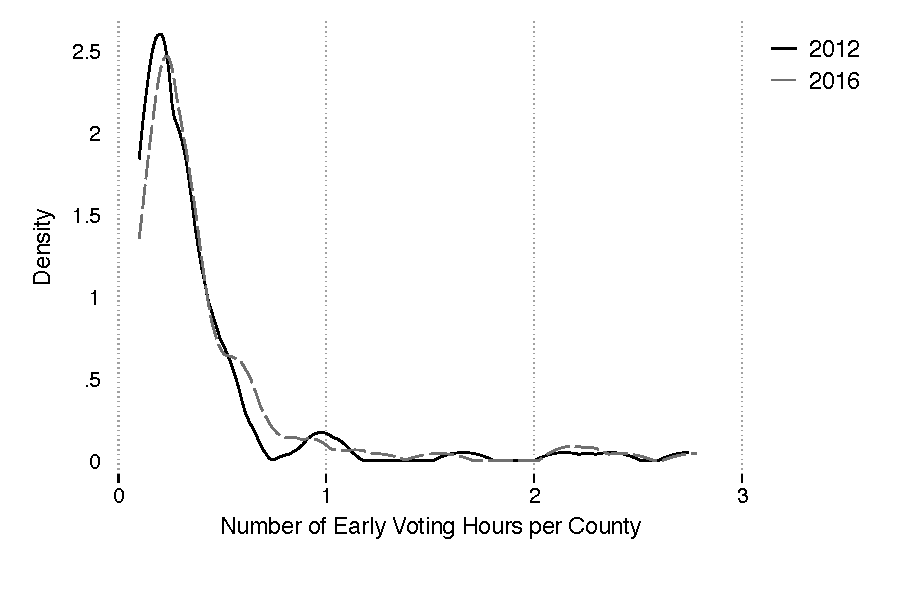
\includegraphics[ width=3in,  clip=true,  trim= 0.0in 0in 0in 0in ]{../../50_results_full/Plot_Distribution_Early_Hours.pdf}
		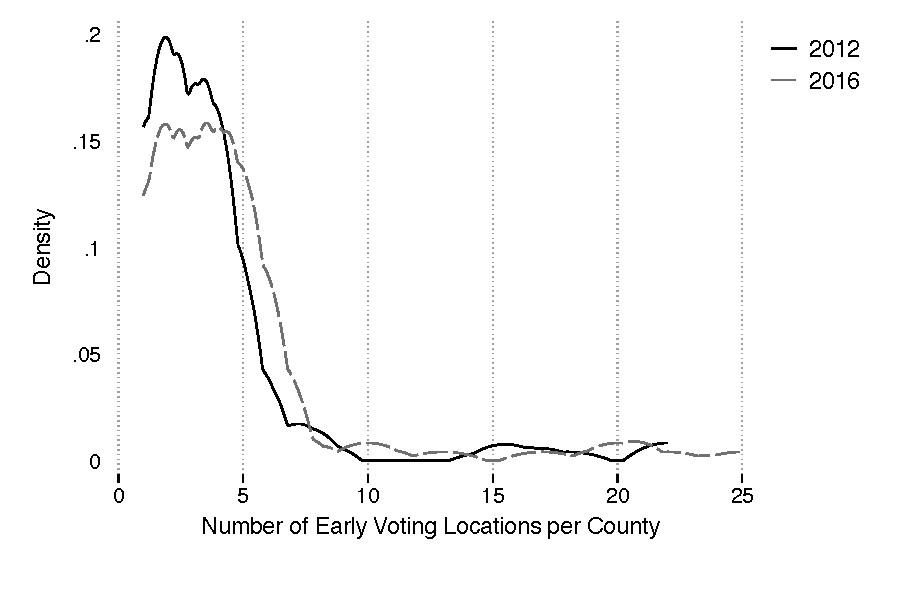
\includegraphics[ width=3in,  clip=true,  trim= 0.0in 0in 0in 0in ]{../../50_results_full/Plot_Distribution_Early_Locations.pdf} \\
		\bigskip
		(c) Weekend Early Voting Hours   \hspace*{1.5in} (d) Evening Early Voting Hours \\
		\smallskip
		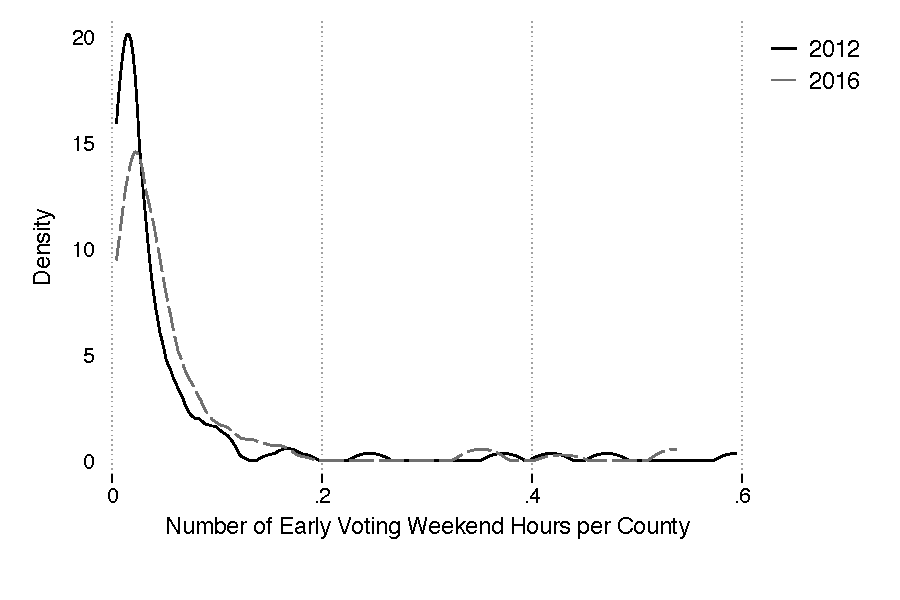
\includegraphics[ width=3in,  clip=true,  trim= 0.0in 0in 0in 0in ]{../../50_results_full/Plot_Distribution_EarlyWeekend.pdf}
		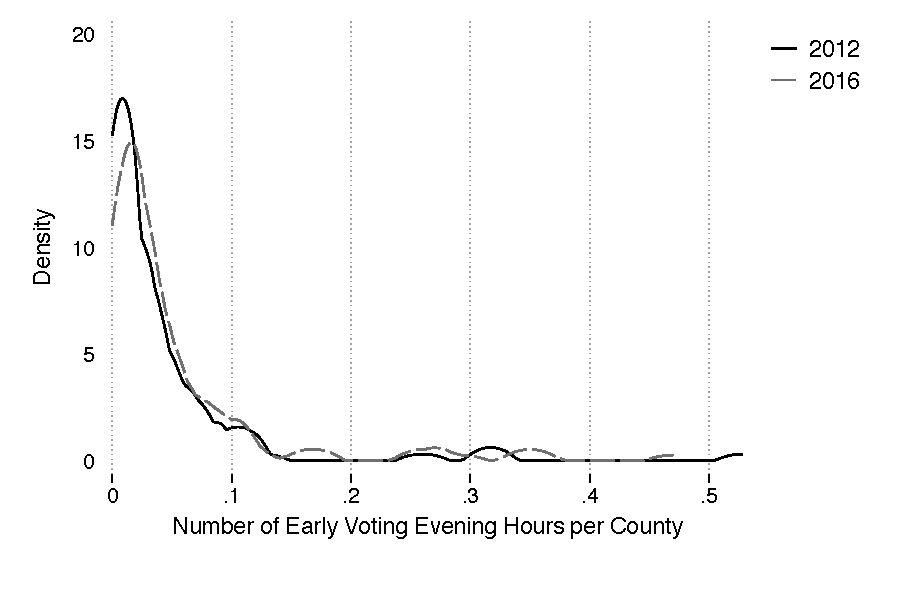
\includegraphics[ width=3in,  clip=true,  trim= 0.0in 0in 0in 0in ]{../../50_results_full/Plot_Distribution_EarlyEvening.pdf} \\
		\label{figure_early_distribution_appendix}
		\end{center}
	\scriptsize{\emph{Notes:}  The above plots present the availability of early voting hours by year (plot (a)) and early voting location by year (plot(b)).  Solid lines are for 2012 (Democrats), and dashed lines are for 2016 (Republicans).  Early voting hours are measured in thousands. }
\end{figure} \normalsize


Given that evening and weekend hours are particularly important for early voting, we re-present the Figure~\ref{figure_scatter_earlyvotingavailability} from the main paper, but examine the relationship between early voting and early voting weekend hours (plot (a)) and early voting evening hours (plot (b)).  (For a thorough description of how the plot is constructed, please see the description in the main body of the paper.)  We see little evidence that more evening early voting hours nor more weekend early voting hours are associated with higher rates of early voting when voters experience a polling place change.

Because neither the scatterplots presented in the paper, nor the plots here show any evidence of a statistically significant relationship between early voting availability and the probability of early voting, we forgo formally estimating the relationship.



%% FIGURE: Changes to Early Voting Availability by Year
%%------------------------------------------------------
\begin{figure}[h!]
	\begin{center}
	\caption{Scatterplot of the Relationship Between 2012 and 2016 Early Voting Availability}
		\small \vspace*{.05in}
		(a) Total Early Voting Hours   \hspace*{1.9in} (b) Early Voting Locations \\
		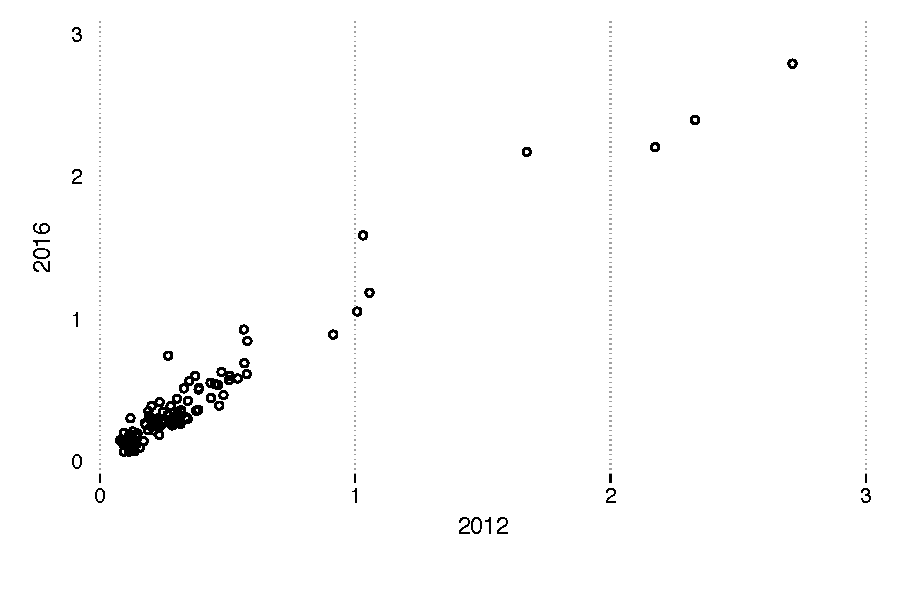
\includegraphics[ width=3in,  clip=true,  trim= 0.0in 0in 0in 0in ]{../../50_results_full/Plot_Scatter_total_hours_2012_vs_2016.pdf}
		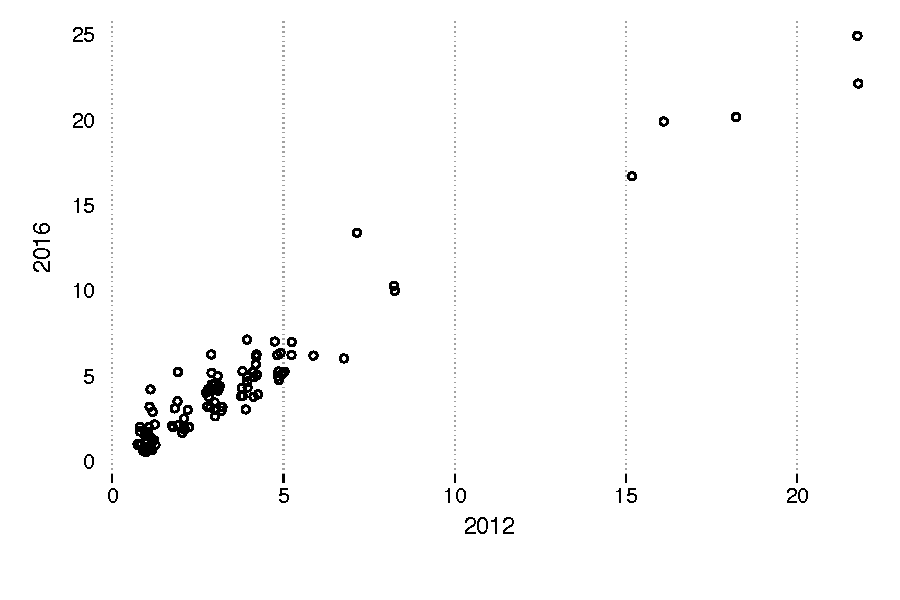
\includegraphics[ width=3in,  clip=true,  trim= 0.0in 0in 0in 0in ]{../../50_results_full/Plot_Scatter_number_of_sites_2012_vs_2016.pdf} \\
		\bigskip
		(c) Weekend Early Voting Hours   \hspace*{1.5in} (d) Evening Early Voting Hours \\
		\smallskip
		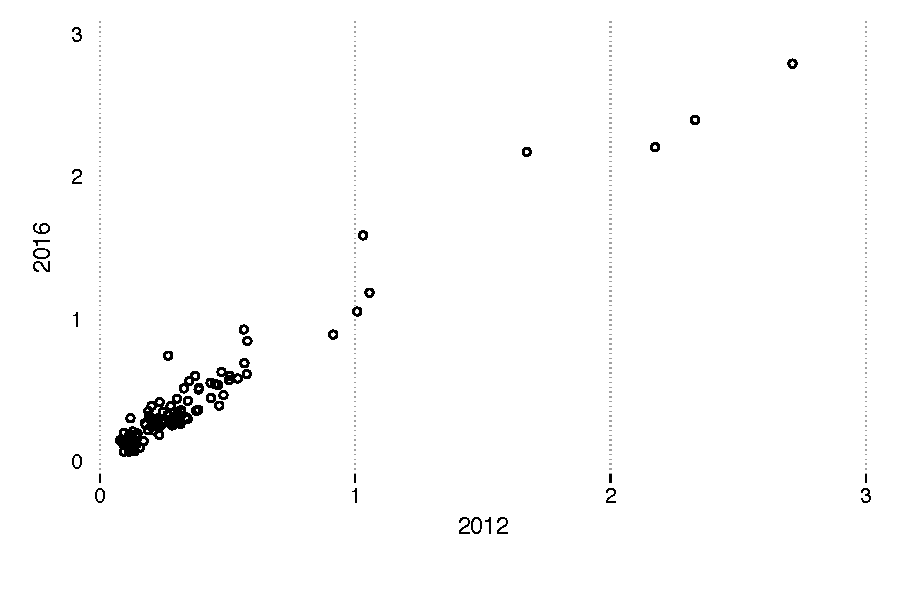
\includegraphics[ width=3in,  clip=true,  trim= 0.0in 0in 0in 0in ]{../../50_results_full/Plot_Scatter_total_hours_2012_vs_2016.pdf}
		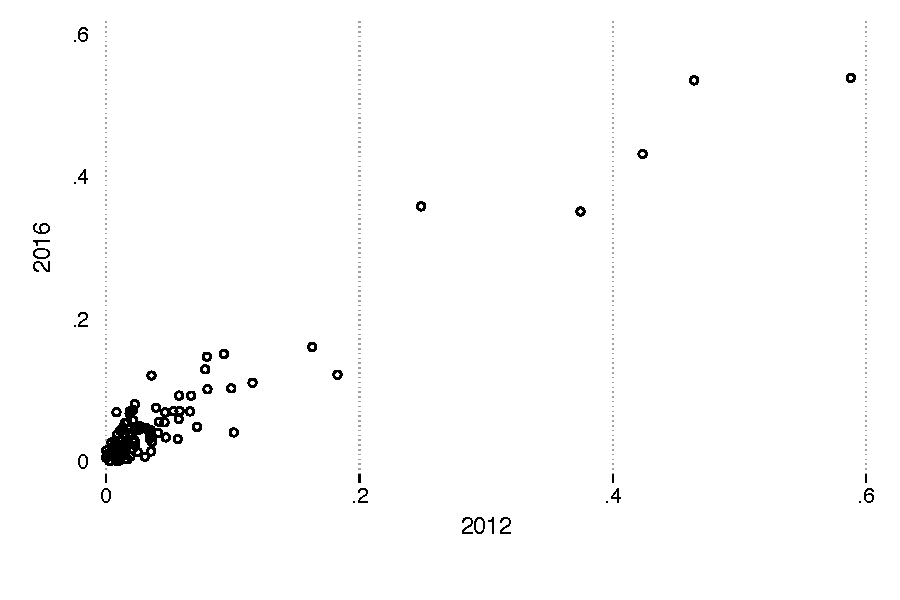
\includegraphics[ width=3in,  clip=true,  trim= 0.0in 0in 0in 0in ]{../../50_results_full/Plot_Scatter_weekend_2012_vs_2016.pdf} \\
		\label{figure_early_scatter_appendix}
		\end{center}
	\scriptsize{\emph{Notes:}  The above plots present scatterplots relating the availability of early voting in 2012 to 2016.  Early voting hours are measured in thousands. }
\end{figure} \normalsize





%  FIGURE: Scatterplots for Early Voting Evenings and Weekends
%-------------------------------------------------------------
\begin{figure}[h!]
	\begin{center}
	\caption{Relationship Between Weekend and Evening Early Voting Hours and Early Voting by Year}
		\small \vspace*{.05in}
		\bigskip
		\hspace*{.4in} (a) Weekend Early Voting Hours  \hspace*{1.0in} (b) Evening Early Voting Hours \\
				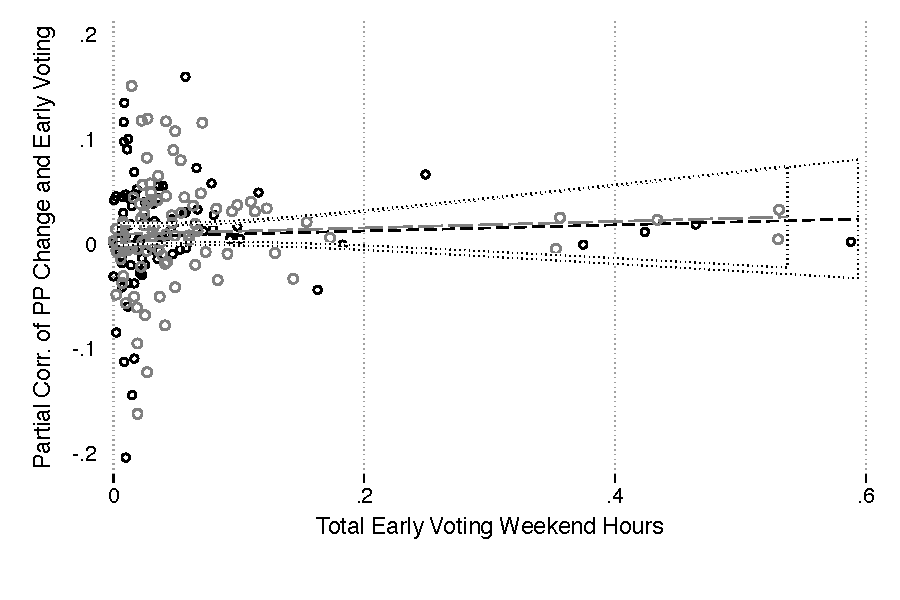
\includegraphics[ width=3in,  clip=true,  trim= 0.0in 0in 0in 0in ]{../../50_results_full/Plot_Scatter_EarlyWeekend_EarlyVote.pdf}
				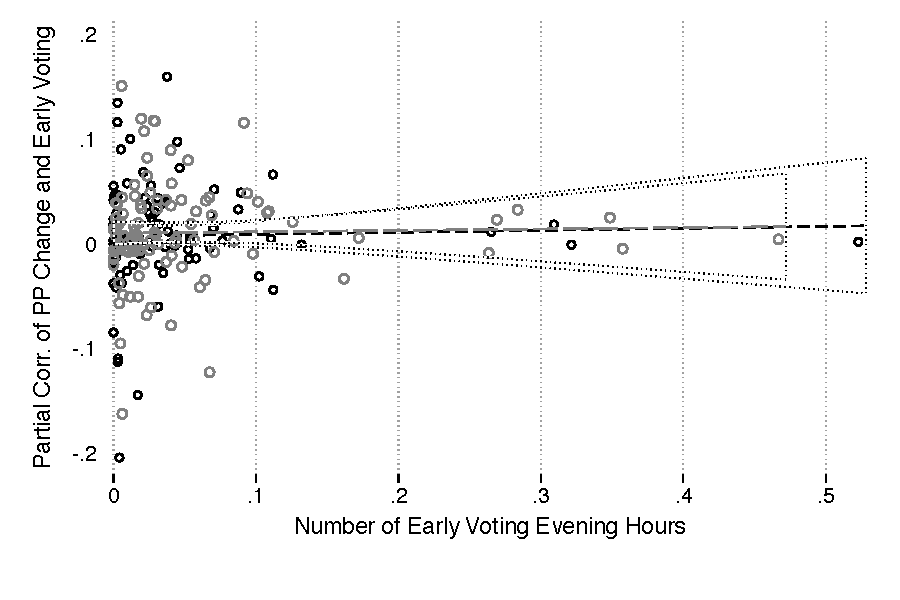
\includegraphics[ width=3in,  clip=true,  trim= 0.0in 0in 0in 0in ]{../../50_results_full/Plot_Scatter_EarlyEvening_EarlyVote.pdf} \\ \vspace*{-.12in}
				%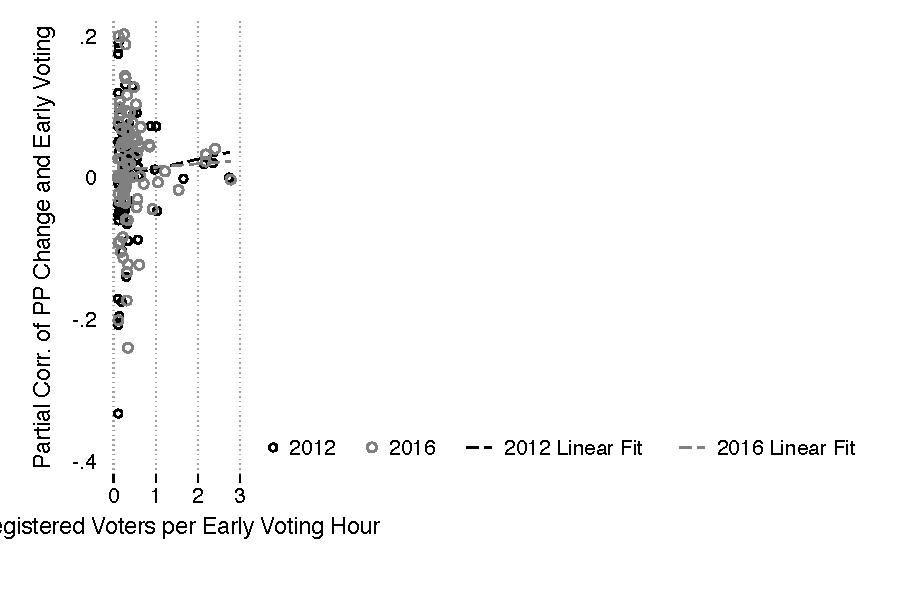
\includegraphics[ width=3.5in,  clip=true,  trim= 0.0in .11in 0in 3.3in ]{../../50_results_full/Plot_Scatter_EarlyHours_Legend.pdf} \vspace*{-.1in}
		\label{figure_scatter_earlyvotingavailability_appendix}
		\end{center}
	\scriptsize{\emph{Notes:}   Plot (a) represents the relationship between the number of weekend early voting hours and the average effect of a polling place change on early voting by county.  Plot (b) represents the relationship between the number of evening early voting hours and the average effect of a polling place change on early voting by county.  Early voting hours are measured in thousands.  The average affect of a polling place on early voting by county is $\beta$ obtained by estimating~\ref{equation_aggregate_crosssectional_closefurther} separately for each county using the outcome of $Pr(VoteEarly)$.  Points in the plots are jittered slightly to aid visualization.  Linear fits are plotted with 95\% confidence intervals.     }
\end{figure} \normalsize


Lastly, we investigate whether normalizing our measure of early voting availability affect our conclusions about whether early voting availability moderates the effect of a polling place change.  One early voting site in a populous county might have less of an effect than one early voting site in a less populous county.  The same is true of hours.  Voters might face longer lines, for instance, if there are few locations or few hours relative to the population size.  We present the scatter plots in Figure~\ref{figure_scatter_earlyvotingavailability} from the main paper, along with the plots from Figure~\ref{figure_scatter_earlyvotingavailability_appendix} in Figure~\ref{figure_scatter_earlyvotingavailability_appendix_normalized} below.  The measures of early voting availability below are normalized by the number of registered eligible voters (from our sample) in the county (i.e. hours per voter, etc.).

Although we observe more variation in the normalized versions of our early voting variables, we do not observe a different pattern in the relationship between early voting availability and early voting conditional on having a polling place change.  From these plots and those presented in the main paper, we cannot but conclude that we cannot detect a statistically significant conditioning effect of early voting availability on early voting turnout.  In the discussion section of the main paper, we consider why that might be the case.


%  FIGURE: Scatterplots for Normalized Early Voting
%--------------------------------------------------
\begin{figure}[h!]
	\begin{center}
	\caption{Relationship Between Early Voting and Normalized Early Voting Availability by Year}
		\small \vspace*{.05in}
		\bigskip
		\hspace*{.4in} (a) Early Voting Locations  \hspace*{1.0in} (b) Total Early Voting Hours \\
				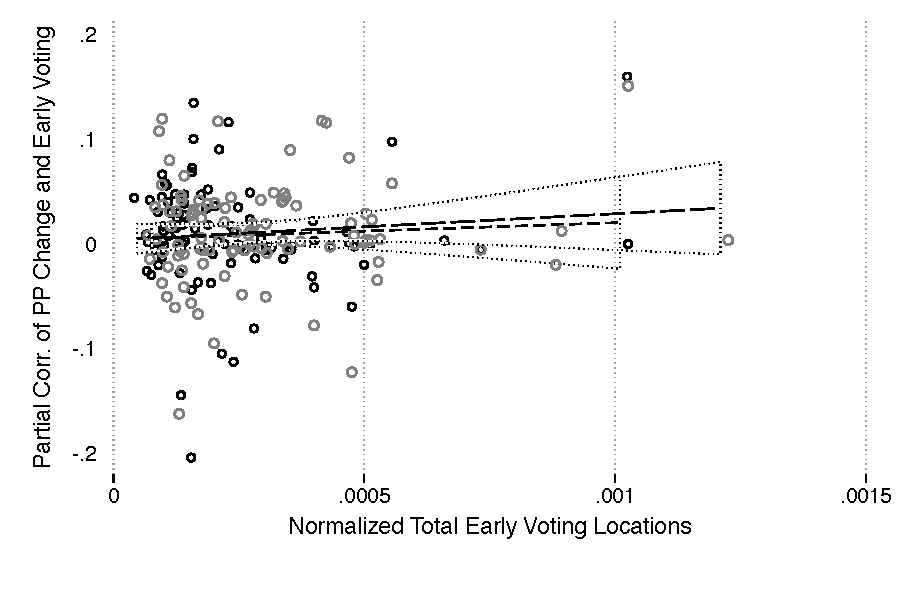
\includegraphics[ width=3in,  clip=true,  trim= 0.0in 0in 0in 0in ]{../../50_results_full/Plot_Scatter_EarlyLocations_EarlyVote_Norm.pdf}
				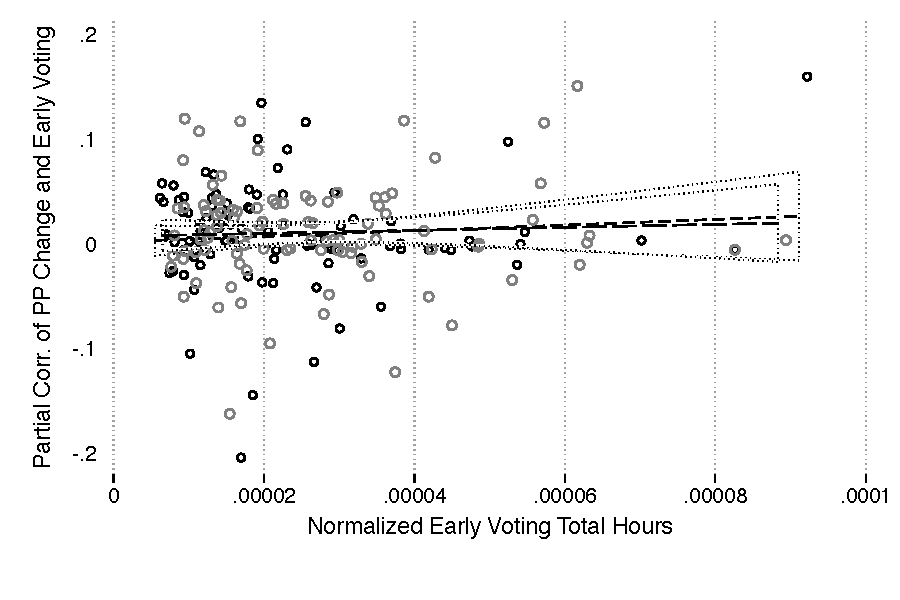
\includegraphics[ width=3in,  clip=true,  trim= 0.0in 0in 0in 0in ]{../../50_results_full/Plot_Scatter_EarlyHours_EarlyVote_Norm.pdf} \\
				\hspace*{.4in} (c) Weekend Early Voting Hours  \hspace*{1.0in} (d) Evening Early Voting Hours \\
				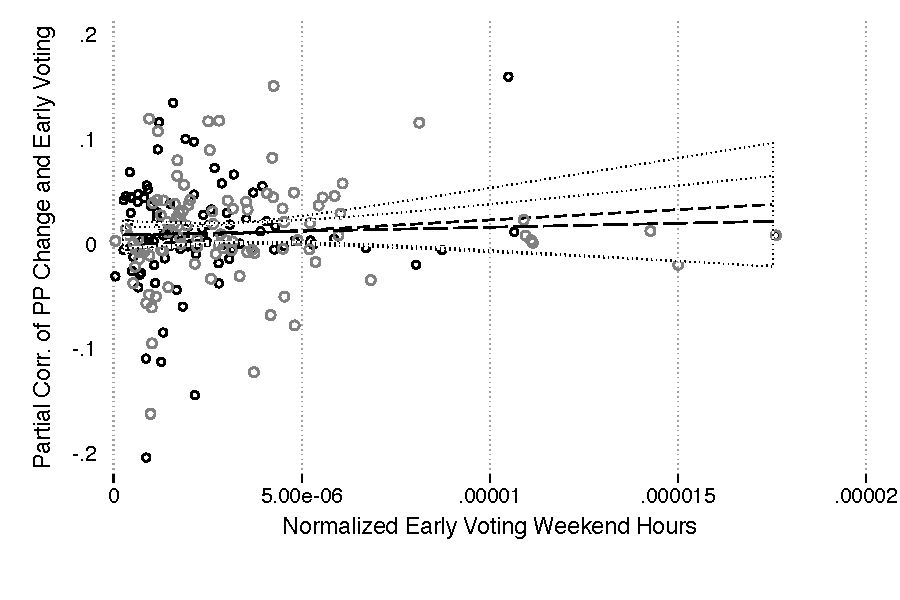
\includegraphics[ width=3in,  clip=true,  trim= 0.0in 0in 0in 0in ]{../../50_results_full/Plot_Scatter_EarlyWeekend_EarlyVote_Norm.pdf}
				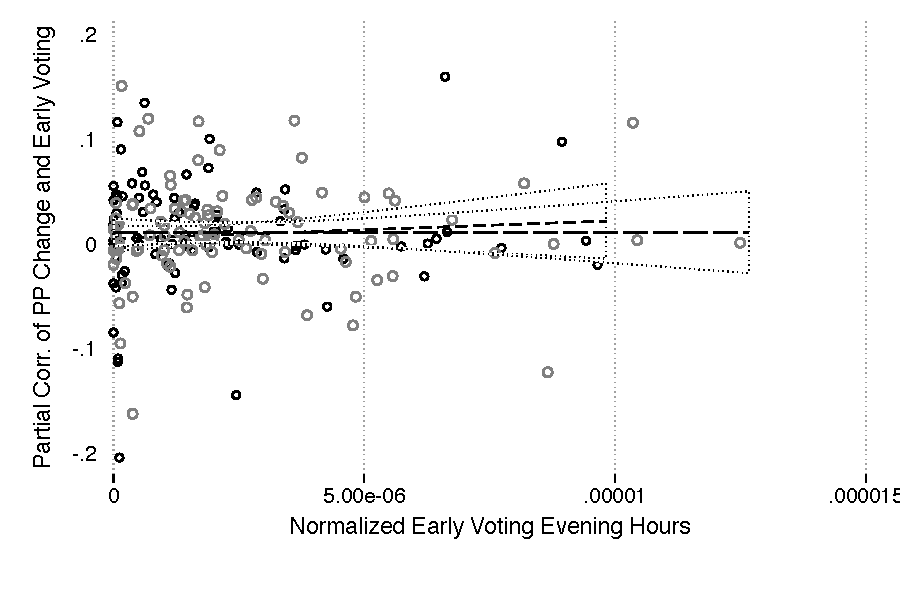
\includegraphics[ width=3in,  clip=true,  trim= 0.0in 0in 0in 0in ]{../../50_results_full/Plot_Scatter_EarlyEvening_EarlyVote_Norm.pdf} \\ \vspace*{-.12in}
		\label{figure_scatter_earlyvotingavailability_appendix_normalized}
		\end{center}
	\scriptsize{\emph{Notes:}   Plot (a) represents the relationship between the number of early voting locations normalized by the number of registered voters and the average effect of a polling place change on early voting by county.  Plot (b) represents the relationship between the total number of early voting hours  normalized by the number of registered voters and the average effect of a polling place change on early voting by county.  Plot (c) represents the relationship between the number of weekend early voting hours  normalized by the number of registered voters and the average effect of a polling place change on early voting by county.  Plot (d) represents the relationship between the number of evening early voting hours  normalized by the number of registered voters and the average effect of a polling place change on early voting by county.  Early voting hours are measured in thousands.  The average affect of a polling place on early voting by county is $\beta$ obtained by estimating~\ref{equation_aggregate_crosssectional_closefurther} separately for each county using the outcome of $Pr(VoteEarly)$.  Points in the plots are jittered slightly to aid visualization.  Linear fits are plotted with 95\% confidence intervals.   We exclude Tyrrell county from the top two plots because it is an extreme outlier given its small population.    }
\end{figure} \normalsize









%--------------------------------------------- APPENDIX K: INCOME ---------------------------------------------%
\clearpage \newpage
\subsection{K. Heterogeneity of Polling Place Change Effects by Income}\label{appendix_incomehetero}
\setcounter{table}{0}
\setcounter{figure}{0}
\renewcommand{\thetable}{K\arabic{table}}
\renewcommand{\thefigure}{K\arabic{figure}}


\noindent In this appendix, we examine whether there is heterogeneity in the effects we estimate in the main paper by the median household income of the census block group.  Our expectation is that voters with lower incomes will have fewer resources to contend with the disruption of a polling place change, and therefore turnout less than voters with higher incomes.  Lacking data on income at the individual level, we use income data at the census block group level.  Although not ideal, this is a very small geographic unit.

Table~\ref{table_pp_panel_income} estimates average effects in our panel by mode of voting.  We find that voters with higher incomes (as measured by the median in the census block group), are more likely to vote on Election Day when their polling place has changed, relative to a voter with lower income.  There is no statistically significant effect for early voting over overall turnout.  These results indicate that while there might be a slight differential response in terms of Election Day voting, there is no difference in overall turnout effects that differ by voter resources.


% TABLE: Heterogeneity in Income, Panel
%--------------------------------------
\begin{table}[h!]\centering \scriptsize
\def\sym#1{\ifmmode^{#1}\else\(^{#1}\)\fi}
	\caption{The Differential Effect of Polling Place Changes on Voter Turnout by Income}\label{table_pp_panel_income}
	\smallskip
	\begin{tabular}{@{\extracolsep{5pt}}l*{4}{c}}
	\noalign{\smallskip}\hline\hline\noalign{\smallskip}\noalign{\smallskip}
			&  \multicolumn{1}{c}{$Pr(VoteElecDay)$} &  \multicolumn{1}{c}{$Pr(VoteEarly)$} &  \multicolumn{1}{c}{$Pr(VoteAny)$}  \\
			\cline{2-4}  \noalign{\smallskip}
				                &\multicolumn{1}{c}{(1)}         &\multicolumn{1}{c}{(2)}         &\multicolumn{1}{c}{(3)}         \\
\midrule
$\Delta$\emph{PollingPlace} $(\hat{\beta})$&   -0.019\sym{***}&    0.013\sym{*}  &  -0.0047         \\
                & (0.0069)         & (0.0070)         & (0.0033)         \\
$\Delta$\emph{PollingPlace}$\cdot Income$&   0.0021         &  -0.0013         &  0.00059         \\
                & (0.0013)         & (0.0012)         &(0.00056)         \\
\midrule
Individual FE   &\checkmark         &\checkmark         &\checkmark         \\
Year FE         &\checkmark         &\checkmark         &\checkmark         \\
County x Year FE&\checkmark         &\checkmark         &\checkmark         \\
Race x Year FE  &\checkmark         &\checkmark         &\checkmark         \\
Year Sample     &Full Panel         &Full Panel         &Full Panel         \\
Observations    &  4680586         &  4680586         &  4680586         \\
Mean of DV      &     0.30         &     0.46         &     0.80         \\
SD of DV        &     0.25         &     0.26         &     0.21         \\
 \\
	\noalign{\vspace*{-.10in}}\hline\hline\noalign{\smallskip}
\multicolumn{4}{p{4.0in}}{\scriptsize Standard errors clustered by precinct assignment history. } \\
\multicolumn{4}{l}{\scriptsize \sym{*} \(p<0.1\), \sym{**} \(p<0.05\), \sym{***} \(p<0.01\)}\\
\multicolumn{4}{p{4.0in}}{\scriptsize  \emph{Notes}: The table presents coefficients from estimating Equation~\ref{equation_traveltime_panel} without the travel time indicators. The unit of analysis is the voter-election.  The SD is the average of the within-$i$ standard deviations of the outcome. }
\end{tabular}
\end{table}


When we turn to examining drive time, we see that there are some differential effects (Table~\ref{table_pp_panel_closefurther_income}).  Those with higher incomes are more likely to turn out on Election Day when their polling place is moved much further away than those with lower incomes who have their polling place moved no more than 5 minutes closer or further from them (column 1).  This results in higher turnout for those with higher incomes who have their polling place moved further away.  Again, this is suggestive that resources allow voters to continue voting on Election Day and continue to turnout in general.




% TABLE: Polling Place Changes and Travel Costs by Mode of Voting and Income
%-----------------------------------------------------------------------------
\begin{table}[h!]\centering \scriptsize
\def\sym#1{\ifmmode^{#1}\else\(^{#1}\)\fi}
	\caption{The Differential Effect of Changes in Travel Time to Polling Place on Turnout by Income}\label{table_pp_panel_closefurther_income}
	\smallskip
	\begin{tabular}{@{\extracolsep{5pt}}l*{4}{c}}
	\noalign{\smallskip}\hline\hline\noalign{\smallskip}\noalign{\smallskip}
			&  \multicolumn{1}{c}{$Pr(VoteElecDay)$} &  \multicolumn{1}{c}{$Pr(VoteEarly)$} &  \multicolumn{1}{c}{$Pr(VoteAny)$}  \\
			\cline{2-4}  \noalign{\smallskip}
				                &\multicolumn{1}{c}{(1)}         &\multicolumn{1}{c}{(2)}         &\multicolumn{1}{c}{(3)}         \\
\midrule
$\Delta$\emph{PollingPlace} $(\hat{\beta})$&   -0.016\sym{**} &    0.012\sym{*}  &  -0.0039         \\
                & (0.0069)         & (0.0070)         & (0.0034)         \\
$\Delta$\emph{PollingPlace}$\cdot Income$&   0.0018         &  -0.0011         &  0.00045         \\
                & (0.0013)         & (0.0012)         &(0.00057)         \\
$\Delta$\emph{MuchCloser} $(\hat{\lambda})$&   -0.013         &   0.0030         &  -0.0099         \\
                &  (0.022)         &  (0.021)         & (0.0099)         \\
$\Delta$\emph{MuchFurther} $(\hat{\delta})$&   -0.059\sym{**} &    0.039         &   -0.021\sym{**} \\
                &  (0.029)         &  (0.027)         & (0.0100)         \\
$\Delta MuchCloser \cdot$\emph{Income}&   0.0048         &  -0.0024         &   0.0022\sym{*}  \\
                & (0.0038)         & (0.0033)         & (0.0012)         \\
$\Delta MuchFurther \cdot$\emph{Income}&   0.0056         &  -0.0026         &   0.0036\sym{**} \\
                & (0.0043)         & (0.0042)         & (0.0016)         \\
\midrule
Individual FE   &\checkmark         &\checkmark         &\checkmark         \\
Year FE         &\checkmark         &\checkmark         &\checkmark         \\
County x Year FE&\checkmark         &\checkmark         &\checkmark         \\
Race x Year FE  &\checkmark         &\checkmark         &\checkmark         \\
Year Sample     &Full Panel         &Full Panel         &Full Panel         \\
Observations    &  4680586         &  4680586         &  4680586         \\
Mean of DV      &     0.30         &     0.46         &     0.80         \\
SD of DV        &     0.25         &     0.26         &     0.21         \\
 \\
	\noalign{\vspace*{-.10in}}\hline\hline\noalign{\smallskip}
\multicolumn{4}{p{4.3in}}{\scriptsize Standard errors clustered by precinct assignment history. } \\
\multicolumn{4}{l}{\scriptsize \sym{*} \(p<0.1\), \sym{**} \(p<0.05\), \sym{***} \(p<0.01\)}\\
\multicolumn{4}{p{4.3in}}{\scriptsize  \emph{Notes}: The table presents coefficients from estimating Equation~\ref{equation_traveltime_panel}. The unit of analysis is the voter-election. The SD is the average of the within-$i$ standard deviations of the outcome.  }
\end{tabular}
\end{table}



The results in Table~\ref{table_pp_crosssec_income} indicate little evidence that income allowed voters to differentially overcome the costs of polling place changes by year.  The interaction between polling place change and income is very small and insignificant in all models.  Although we don't estimate the interacted model to determine if the coefficient on the interaction is statistically \emph{different} between 2012 and 2016, even if it were, the magnitudes would be exceedingly small.

The results from Table~\ref{table_pp_crosssec_closerfurther_income} are similar and suggest that partisan changes between years were moderated by the differential ability of higher relative to lower income voters to overcome costs associated with drive time to their new polling place.


% TABLE: Polling Place Changes by Mode of Voting, Cross-Sectional by Income
%---------------------------------------------------------------------------
\begin{table}[h!]\centering \scriptsize
\def\sym#1{\ifmmode^{#1}\else\(^{#1}\)\fi}
	\caption{The Differential Effect of Polling Place Changes by Year by Income}\label{table_pp_crosssec_income}
	\smallskip
	\begin{tabular}{@{\extracolsep{5pt}}l*{6}{c}}
	\noalign{\smallskip}\hline\hline\noalign{\smallskip}\noalign{\smallskip}
			&  \multicolumn{2}{c}{$Pr(VoteElecDay)$} &  \multicolumn{2}{c}{$Pr(VoteEarly)$} &  \multicolumn{2}{c}{$Pr(VoteAny)$}  \\
			\cline{2-3} \cline{4-5} \cline{6-7} \noalign{\smallskip}
				                &\multicolumn{1}{c}{(1)}         &\multicolumn{1}{c}{(2)}         &\multicolumn{1}{c}{(3)}         &\multicolumn{1}{c}{(4)}         &\multicolumn{1}{c}{(5)}         &\multicolumn{1}{c}{(6)}         \\
\midrule
$\Delta$\emph{PollingPlace} $(\hat{\beta})$&   -0.022\sym{***}&   -0.034\sym{***}&    0.023\sym{**} &    0.029\sym{***}&   0.0027         &  -0.0070         \\
                & (0.0085)         & (0.0086)         &  (0.011)         & (0.0094)         & (0.0051)         & (0.0048)         \\
$\Delta$\emph{PollingPlace}$\cdot Income$&   0.0011         &   0.0012         & -0.00088         &  -0.0010         & -0.00013         &  0.00062         \\
                & (0.0015)         &(0.00079)         & (0.0023)         & (0.0013)         &(0.00089)         &(0.00093)         \\
\emph{Income}   &  -0.0022\sym{***}&  -0.0032\sym{**} &   0.0085\sym{***}&   0.0065\sym{***}&   0.0077\sym{***}&   0.0039\sym{***}\\
                &(0.00062)         & (0.0015)         &(0.00084)         & (0.0015)         &(0.00053)         &(0.00043)         \\
\midrule
County FE       &\checkmark         &\checkmark         &\checkmark         &\checkmark         &\checkmark         &\checkmark         \\
Individual Controls&\checkmark         &\checkmark         &\checkmark         &\checkmark         &\checkmark         &\checkmark         \\
Year Sample     &     2012         &     2016         &     2012         &     2016         &     2012         &     2016         \\
Observations    &  2340293         &  2340293         &  2340293         &  2340293         &  2340293         &  2340293         \\
Mean of DV      &     0.33         &     0.26         &     0.47         &     0.45         &     0.84         &     0.75         \\
SD of DV        &     0.46         &     0.44         &     0.49         &     0.49         &     0.36         &     0.43         \\
 \\
	\noalign{\vspace*{-.10in}}\hline\hline\noalign{\smallskip}
\multicolumn{7}{p{5.2in}}{\scriptsize Robust standard errors in parentheses. } \\
\multicolumn{7}{l}{\scriptsize \sym{*} \(p<0.1\), \sym{**} \(p<0.05\), \sym{***} \(p<0.01\)}\\
\multicolumn{7}{p{5.2in}}{\scriptsize  \emph{Notes}: The table presents coefficients from estimating Equation~\ref{equation_aggregate_crosssectional_closefurther} without the travel time indicators.  The unit of analysis is the voter. The SD is the average of the within-county standard deviations of the outcome.  }
\end{tabular}
\end{table}



% TABLE: Travel Time Changes by Mode of Voting, Cross-Sectional by Income
%------------------------------------------------------------------------
\begin{table}[h!]\centering \scriptsize
\def\sym#1{\ifmmode^{#1}\else\(^{#1}\)\fi}
	\caption{The Differential Effect of Changes in Travel Time to Polling Places by Year by Income}\label{table_pp_crosssec_closerfurther_income}
	\smallskip
	\begin{tabular}{@{\extracolsep{5pt}}l*{6}{c}}
	\noalign{\smallskip}\hline\hline\noalign{\smallskip}\noalign{\smallskip}
			&  \multicolumn{2}{c}{$Pr(VoteElecDay)$} &  \multicolumn{2}{c}{$Pr(VoteEarly)$} &  \multicolumn{2}{c}{$Pr(VoteAny)$}  \\
			\cline{2-3} \cline{4-5} \cline{6-7} \noalign{\smallskip}
				                &\multicolumn{1}{c}{(1)}         &\multicolumn{1}{c}{(2)}         &\multicolumn{1}{c}{(3)}         &\multicolumn{1}{c}{(4)}         &\multicolumn{1}{c}{(5)}         &\multicolumn{1}{c}{(6)}         \\
\midrule
$\Delta$\emph{PollingPlace} $(\hat{\beta})$&   -0.013         &   -0.018\sym{*}  &   -0.012         & -0.00044         &   -0.029\sym{***}&   -0.022\sym{***}\\
                & (0.0091)         & (0.0097)         &  (0.011)         &  (0.012)         & (0.0056)         & (0.0049)         \\
$\Delta$\emph{PollingPlace}$\cdot Income$& -0.00061         &  -0.0017         &   0.0056\sym{**} &   0.0044\sym{**} &   0.0056\sym{***}&   0.0036\sym{***}\\
                & (0.0016)         & (0.0012)         & (0.0025)         & (0.0021)         &(0.00097)         &(0.00098)         \\
$\Delta$\emph{MuchCloser} $(\hat{\lambda})$&   0.0091         &   0.0044         &  -0.0022         &  -0.0081         &   0.0028         & -0.00036         \\
                &  (0.021)         &  (0.019)         &  (0.020)         &  (0.014)         &  (0.012)         & (0.0082)         \\
$\Delta$\emph{MuchFurther} $(\hat{\delta})$&  -0.0060         &   -0.029         &    0.012         &    0.018         &   0.0070         &  -0.0075         \\
                &  (0.016)         &  (0.033)         &  (0.016)         &  (0.038)         &  (0.011)         &  (0.012)         \\
$\Delta MuchCloser \cdot$\emph{Income}&   0.0011         &   0.0036         &  -0.0014         &  -0.0042\sym{**} & -0.00017         & -0.00071         \\
                & (0.0034)         & (0.0022)         & (0.0040)         & (0.0018)         & (0.0014)         & (0.0012)         \\
$\Delta MuchFurther \cdot$\emph{Income}& -0.00042         &  -0.0036         &-0.000035         &   0.0047         & -0.00021         &  0.00025         \\
                & (0.0021)         & (0.0050)         & (0.0027)         & (0.0055)         & (0.0018)         & (0.0018)         \\
\midrule
County FE       &\checkmark         &\checkmark         &\checkmark         &\checkmark         &\checkmark         &\checkmark         \\
Individual Controls&\checkmark         &\checkmark         &\checkmark         &\checkmark         &\checkmark         &\checkmark         \\
Year Sample     &     2012         &     2016         &     2012         &     2016         &     2012         &     2016         \\
Observations    &  2340293         &  2340293         &  2340293         &  2340293         &  2340293         &  2340293         \\
Mean of DV      &     0.33         &     0.26         &     0.47         &     0.45         &     0.84         &     0.75         \\
SD of DV        &     0.46         &     0.44         &     0.49         &     0.49         &     0.36         &     0.43         \\
 \\
	\noalign{\vspace*{-.10in}}\hline\hline\noalign{\smallskip}
\multicolumn{7}{p{5.4in}}{\scriptsize Robust standard errors in parentheses. } \\
\multicolumn{7}{l}{\scriptsize \sym{*} \(p<0.1\), \sym{**} \(p<0.05\), \sym{***} \(p<0.01\)}\\
\multicolumn{7}{p{5.4in}}{\scriptsize  \emph{Notes}: The table presents coefficients from estimating equation~~\ref{equation_aggregate_crosssectional_closefurther}.  The unit of analysis is the voter. The SD is the average of the within-county standard deviations of the outcome.  }
\end{tabular}
\end{table}



%------------------------------------------ APPENDIX L: Geocoding --------------------------------------%
\clearpage \newpage
\subsection{L. Details of the Geocoding Procedure}\label{appendix_geocoding}
\setcounter{table}{0}
\setcounter{figure}{0}
\renewcommand{\thetable}{L\arabic{table}}
\renewcommand{\thefigure}{L\arabic{figure}}



\noindent Data on 2008 polling places come from the NCSBE data archives -- snapshot date: April 3rd, 2008 --  data on 2012 polling places come from the Data Director of the North Carolina Democratic Party, and data on 2016 polling places were collected from the mid-2017 Internet Archives image of the NCSBE Polling Place Search website.

Shapefiles of precinct boundaries were collected from the NCSBE website for 2012 and 2016 -- snapshot dates: October 4th, 2016 for 2016 election; September 1st, 2012 for 2012 -- and from the NCSBE 2008 precinct boundary shapefile submitted to the 2011 redistricting database to associate polling places and precincts. In some cases, poor record keeping combined with the fact that not all polling places are located with the borders of the precinct they serve makes it impossible to ascertain the precinct served by a given polling places. When a precinct's polling place cannot be ascertained with certainty, we drop that precinct from the analysis. This generates a sample of    3,362,808\unskip~voters with a geolocated polling place, or      79.1\unskip\%~of voters with accurate residence geocodes.




%%------------------------------ SECTION: Partisan ----------------------------------- %%
\clearpage \newpage
\subsection{M. Partisan-Controlled Polling Place Changes}\label{appendix_partisan}
\setcounter{table}{0}
\setcounter{figure}{0}
\renewcommand{\thetable}{M\arabic{table}}
\renewcommand{\thefigure}{M\arabic{figure}}

\noindent Polling place changes made between 2008 and 2012 were made by Democrat-selected local election administrators, while polling place changes made between 2012 and 2016 were made by Republican-selected administrators.  In the main manuscript, we suggest why there is limited theoretical expectation that polling place changes made under different partisan regimes should impact turnout.  However, we might expect the intentions to differ by these partisan administrators, the voters targeted to differ, their resources to overcome the imposed costs to differ, and therefore the state-wide turnout effects to differ as well. If so, the average effects we identify may obscure important differences in the effects of the polling place changes made by different regimes of partisan-appointed election administrators.

Even if such partisan motivations exist, however, the ability of such changes to differentially affect turnout is theoretically unclear.  If, for example, search costs, confusion, and habit disruption are more consequential than travel costs, than \emph{any} change in polling place location may produce similar turnout effects.  Put differently, attempts to increase turnout by decreasing travel costs by moving or adding polling places may be undermined by the the resulting search costs, confusion, and habit disruption produced by such changes.





% Republicans also cut 27 polling places for the 2016 presidential election \citep{leadershipcoun2016}, but this was a small fraction of the 3,121 polling places in 2012.



To estimate the impact of polling place changes under different election administration regimes, we separately estimate the impact of polling place changes made between 2008 and 2012 on 2012 turnout and the effects of changes made between 2012 and 2016 on 2016 turnout. We estimate these cross-sectional regressions using a comprehensive set of voter-level covariates and county fixed effects to leverage within-county variation and control for stable county-level features such as population, density, and urban/rural composition that may affect turnout decisions.

Because of our balanced panel, we analyze the same voters in each time period --- an important consideration that helps eliminate any confounding effects caused by \emph{compositional} changes in the electorate over time. Even so, comparing the impact of polling place changes between the two time periods is unfortunately and unavoidably confounded by the potential impact of other temporal differences that may be correlated with polling place changes. It is unclear what these time-varying and highly correlated factors might be, but we acknowledge that factors other than partisanship may affects the effect of the polling place changes we examine.

To estimate the effects of Democrat-led and Republican-led polling place changes we estimate the following equation separately for 2012 and 2016:
\begin{align}\label{equation_aggregate_crosssectional_closefurther}
	Pr(Vote_{i,c}) = \eta_{c} + \beta \Delta PollingPlace_{i,c} + \delta \Delta MuchFurther_{i,c} + \lambda \Delta MuchCloser_{i,c}  \\
    + \boldsymbol{\psi Vote}_{i,c,t-1} +   \boldsymbol{\kappa X}_{i,c}  + \epsilon_{i,c} \nonumber
\end{align}

where $\eta_{c}$ are county-level fixed effects, and $\boldsymbol{X}$ is a vector of covariates that we use to account for individual characteristics affecting the decision to turnout, including race, partisan identification, age, age squared, gender, and median household income at the 2010 census block. The remaining variables are measured as in equation~\ref{equation_traveltime_panel}.  We cluster our robust standard errors at the county level to account for common shocks to individuals within the same county and the heteroskedasticity of the linear probability model we employ.  As before, we estimate equation~\ref{equation_aggregate_crosssectional_closefurther} for each mode turnout, and with and without the travel time indicators.



% TABLE 6: Polling Place Changes by Mode of Voting, Cross-Sectional
%-------------------------------------------------------------------
\begin{table}[t!]\centering \footnotesize
\def\sym#1{\ifmmode^{#1}\else\(^{#1}\)\fi}
	\caption{The Differential Effects of Polling Place Changes by Year}\label{table_pp_crosssec}
	\smallskip
	\begin{tabular}{@{\extracolsep{5pt}}l*{6}{c}}
	\noalign{\smallskip}\hline\hline\noalign{\smallskip}\noalign{\smallskip}
			&  \multicolumn{2}{c}{$Pr(VoteElecDay)$} &  \multicolumn{2}{c}{$Pr(VoteEarly)$} &  \multicolumn{2}{c}{$Pr(VoteAny)$}  \\
			\cline{2-3} \cline{4-5} \cline{6-7} \noalign{\smallskip}
				                &\multicolumn{1}{c}{(1)}         &\multicolumn{1}{c}{(2)}         &\multicolumn{1}{c}{(3)}         &\multicolumn{1}{c}{(4)}         &\multicolumn{1}{c}{(5)}         &\multicolumn{1}{c}{(6)}         \\
\midrule
$\Delta$\emph{PollingPlace} $(\hat{\beta})$&   -0.016\sym{***}&   -0.028\sym{***}&    0.019\sym{***}&    0.023\sym{***}&   0.0020         &  -0.0037\sym{**} \\
                & (0.0035)         & (0.0059)         & (0.0045)         & (0.0055)         & (0.0024)         & (0.0018)         \\
\midrule
County FE       &\checkmark         &\checkmark         &\checkmark         &\checkmark         &\checkmark         &\checkmark         \\
Individual Controls&\checkmark         &\checkmark         &\checkmark         &\checkmark         &\checkmark         &\checkmark         \\
Year Sample     &     2012         &     2016         &     2012         &     2016         &     2012         &     2016         \\
Observations    &  2340293         &  2340293         &  2340293         &  2340293         &  2340293         &  2340293         \\
Mean of DV      &     0.33         &     0.26         &     0.47         &     0.45         &     0.84         &     0.75         \\
SD of DV        &     0.46         &     0.44         &     0.49         &     0.49         &     0.36         &     0.43         \\
 \\
	\noalign{\vspace*{-.17in}}\hline\hline\noalign{\smallskip}
\multicolumn{7}{p{5.6in}}{\scriptsize Standard errors clustered at the individual level. } \\
\multicolumn{7}{l}{\scriptsize \sym{*} \(p<0.1\), \sym{**} \(p<0.05\), \sym{***} \(p<0.01\)}\\
\multicolumn{7}{p{5.4in}}{\scriptsize  \emph{Notes}: The table presents coefficients from estimating Equation~\ref{equation_aggregate_crosssectional_closefurther} without the drive time indicators.  The unit of analysis is the voter-election.  See Table~\ref{table_pp_crosssec_wcontrols} in Appendix C for the full set of coefficient estimates.}
\end{tabular}
\end{table}

Table~\ref{table_pp_crosssec} presents the results of the effect of a polling place change unconditioned by changing travel time.  As in our panel results (Table~\ref{table_pp_panel}), both Democrat and Republican-led polling place changes decrease Election Day turnout, although the decline is much larger for Republican-led changes. Comparing the effects of Democrats (column 1) and Republicans (column 2) reveals a decline of     -1.6 percentage points under Democrats and    -2.8 percentage points under Republicans.

% If Democrat-led changes were attempting to increase Election Day turnout by moving polling place locations -- and the fact that registered Democrats and black voters were slightly more likely to be impacted under Democrat-led changes would be consistent with this motivation -- they were not successful in those attempts because neither Election Day voting nor overall turnout increase under Democrat-led changes.



Consistent with our previous panel findings, the decrease in Election Day vote that we identify is accompanied by a similarly sized increase in early voting across \emph{both} years (columns 3 and 4) ---     1.9 percentage points under Democrats and     2.3 percentage points under Republicans.  However, the Election Day and early voting effects are not completely offsetting for Republican-led changes.  Columns 5 and 6 reveal that although voters substitute from Election Day voting to early voting occurs in response to both partisan changes, the Republican-controlled changes were substantial enough to reduce \emph{overall} voter turnout by    -0.4 percentage points (column 6).  Estimating a model that interacts the effect of polling place change with year (as opposed to splitting the sample) allows us to reject the null hypothesis that the effect of a polling place change in Election Day voting and on overall turnout is the same between the two years.  We fail to reject that null hypothesis for early voting.  If Democrat-led changes were attempting to increase Election Day turnout by moving polling place locations closer to likely supporters, our results indicate that these attempts were unsuccessful.  %[X Adriane: Do you want to put those results in an Appendix...?  Not really, because it's tedious and time consuming.  But maybe you should.]

Because search costs, confusion, and habit disruption arguably occur whenever a polling place change occurs, we might expect the largest differences in partisan effects to occur in terms of the effects of travel costs. (Table \ref{table_substitution_v_composition} in Appendix G already suggests that there are not different overall average effects on turnout by party registration.)  In particular, Democratic supporters tend to be concentrated amongst racial minorities and less resourced voters who arguably benefit more from a polling place being moved closer to them than rural Republican voters who live in more expansive precincts --- if so, the effects of travel costs may vary depending on the party in control of the process of selecting polling places.



% TABLE: Travel Time Changes by Mode of Voting, Cross-Sectional
%--------------------------------------------------------------
\begin{table}[t!]\centering \footnotesize
\def\sym#1{\ifmmode^{#1}\else\(^{#1}\)\fi}
	\caption{The Differential Effects of Changes in Travel Time to Polling Places by Year}\label{table_pp_crosssec_closerfurther}
	\smallskip
	\begin{tabular}{@{\extracolsep{5pt}}l*{6}{c}}
	\noalign{\smallskip}\hline\hline\noalign{\smallskip}\noalign{\smallskip}
			&  \multicolumn{2}{c}{$Pr(VoteElecDay)$} &  \multicolumn{2}{c}{$Pr(VoteEarly)$} &  \multicolumn{2}{c}{$Pr(VoteAny)$}  \\
			\cline{2-3} \cline{4-5} \cline{6-7} \noalign{\smallskip}
				                &\multicolumn{1}{c}{(1)}         &\multicolumn{1}{c}{(2)}         &\multicolumn{1}{c}{(3)}         &\multicolumn{1}{c}{(4)}         &\multicolumn{1}{c}{(5)}         &\multicolumn{1}{c}{(6)}         \\
\midrule
$\Delta$\emph{MuchCloser} $(\hat{\lambda})$&    0.017         &    0.026\sym{***}&   -0.013         &   -0.033\sym{***}&  0.00016         &  -0.0039         \\
                &  (0.015)         & (0.0087)         &  (0.014)         & (0.0093)         & (0.0048)         & (0.0050)         \\
$\Delta$\emph{MuchFurther} $(\hat{\delta})$&  -0.0077         &   -0.045\sym{***}&   0.0095         &    0.039\sym{**} &   0.0044         &  -0.0073         \\
                & (0.0075)         &  (0.016)         & (0.0075)         &  (0.019)         & (0.0048)         & (0.0045)         \\
$\Delta$\emph{PollingPlace} $(\hat{\beta})$&   -0.017\sym{***}&   -0.027\sym{***}&    0.019\sym{***}&    0.023\sym{***}&   0.0018         &  -0.0033\sym{*}  \\
                & (0.0034)         & (0.0055)         & (0.0045)         & (0.0051)         & (0.0025)         & (0.0018)         \\
\midrule
County FE       &\checkmark         &\checkmark         &\checkmark         &\checkmark         &\checkmark         &\checkmark         \\
Individual Controls&\checkmark         &\checkmark         &\checkmark         &\checkmark         &\checkmark         &\checkmark         \\
Year Sample     &     2012         &     2016         &     2012         &     2016         &     2012         &     2016         \\
Observations    &  2340293         &  2340293         &  2340293         &  2340293         &  2340293         &  2340293         \\
Mean of DV      &     0.33         &     0.26         &     0.47         &     0.45         &     0.84         &     0.75         \\
SD of DV        &     0.46         &     0.44         &     0.49         &     0.49         &     0.36         &     0.43         \\
 \\
	\noalign{\vspace*{-.17in}}\hline\hline\noalign{\smallskip}
\multicolumn{7}{p{5.4in}}{\scriptsize Robust standard errors in parentheses. } \\
\multicolumn{7}{l}{\scriptsize \sym{*} \(p<0.1\), \sym{**} \(p<0.05\), \sym{***} \(p<0.01\)}\\
\multicolumn{7}{p{5.4in}}{\scriptsize  \emph{Notes}: The table presents coefficients from estimating Equation~\ref{equation_aggregate_crosssectional_closefurther}.  The unit of analysis is the voter.   See Table~\ref{table_pp_crosssec_closerfurther_wcontrols} in Appendix C for the full set of coefficient estimates.  The SD of the DV is the average of the within-county standard deviations of the outcome.}
\end{tabular}
\end{table}

Table~\ref{table_pp_crosssec_closerfurther} presents the results from estimating equation~\ref{equation_aggregate_crosssectional_closefurther} with indicators for travel time.  We find some evidence that the impact of travel costs depends on the party in control of the process.  Election Day voting increases when polling places are moved much closer to voters, and declines when they're moved much further away (relative to small changes in travel time), but only for Republican-led changes in 2016 (column 2).  But even though the differential effects ($\hat{\lambda}$) are distinguishable from zero, the net effect of a polling place being moved much closer on Election Day voting, even in 2016, (i.e., $\hat{\beta} + \hat{\lambda}$) is still nearly exactly zero.

The results for early voting reverse this pattern and again show evidence of substitution.  But again, this substitution is only evident for Republican-led changes (column 4).  Voters moved much closer to their polling place in 2016 are less likely to vote early, while those moved much further away are more likely to do so.  However, even given differential substitution, we find no differential net turnout effects conditional on drive time between the two partisan regimes (column 5 and 6).  Although the fact that the effect of a polling place change of any kind ($\hat{\beta}$) is distinguishable from zero for Republican-led changes in 2016 (column 6) reveals that the polling place changes introduced by Republicans slightly decreased overall turnout. Estimating an interacted model to assess whether the coefficients are the same across years further reveals that only in the case of the probability of early voting and a polling place being moved much further is there statistically significant difference in the effects under partisan regimes --- voters are slightly more likely to turnout early when their polling place is moved much further in 2016 (by Republicans) than in 2012 (by Democrats).





%%------------------------------ SECTION: Lead Regressions ----------------------------------- %%
\clearpage \newpage
\subsection{N. Predicting 2012 Turnout with Future Polling Place Changes}\label{appendix_lead}
\setcounter{table}{0}
\setcounter{figure}{0}
\renewcommand{\thetable}{N\arabic{table}}
\renewcommand{\thefigure}{N\arabic{figure}}


\noindent In this appendix we offer one additional test to provide additional evidence on the strength of our counterfactual assumption --- that is, that the behavior of individuals who experienced a polling place change prior to a given election \emph{would have been the same} had they not experienced that change.  Although a standard test for parallel trends in our setting without a discrete pre and post treatment period is not possible, we can nevertheless examine whether future polling place changes are correlated with past turnout behavior, after accounting for past polling place changes, county characteristics, and individual level characteristic.  Once we have taken into account past and fixed behavior, we should not expect future changes to be related to past behavior.

With only two time periods of polling place changes --- 2008-2012 and 2012-2016 --- we can only provide evidence on whether changes from 2012-2016 predict 2012 behavior, after accounting for county fixed effects and individual covariates.  This cross-sectional specification is not our preferred specification, as it does not allow us to use our most rigorous set of fixed effects (e.g. individual voter fixed effects), but it still provides potentially useful, albeit imperfect, evidence.


% TABLE: Travel Time Changes by Mode of Voting, Cross-Sectional
%--------------------------------------------------------------
\begin{table}[h!]\centering \footnotesize
\def\sym#1{\ifmmode^{#1}\else\(^{#1}\)\fi}
	\caption{Predicting 2012 Turnout with Preceding and Future Polling Place Changes}\label{table_pp_lead}
	\smallskip
	\begin{tabular}{@{\extracolsep{5pt}}l*{3}{c}}
	\noalign{\smallskip}\hline\hline\noalign{\smallskip}\noalign{\smallskip}
			&  \multicolumn{1}{c}{$Pr(VoteElecDay)$} &  \multicolumn{1}{c}{$Pr(VoteEarly)$} &  \multicolumn{1}{c}{$Pr(VoteAny)$}  \\
			\cline{2-4}  \noalign{\smallskip}
				                &\multicolumn{1}{c}{(1)}         &\multicolumn{1}{c}{(2)}         &\multicolumn{1}{c}{(3)}         \\
\midrule
$\Delta$\emph{PollingPlace} $(\hat{\beta})$&   -0.016\sym{***}&    0.018\sym{***}&   0.0022         \\
                & (0.0035)         & (0.0044)         & (0.0024)         \\
$\Delta$\emph{Polling Place (lead, 2012-2016)}&   -0.011\sym{**} &   0.0066         &  -0.0035         \\
                & (0.0049)         & (0.0055)         & (0.0021)         \\
\midrule
County FE       &\checkmark         &\checkmark         &\checkmark         \\
Individual Controls&\checkmark         &\checkmark         &\checkmark         \\
Year Sample     &     2012         &     2012         &     2012         \\
Observations    &  2340293         &  2340293         &  2340293         \\
Mean of DV      &     0.33         &     0.33         &     0.47         \\
SD of DV        &     0.46         &     0.46         &     0.49         \\
 \\
	\noalign{\vspace*{-.17in}}\hline\hline\noalign{\smallskip}
\multicolumn{4}{p{5.3in}}{\scriptsize Robust standard errors in parentheses. } \\
\multicolumn{4}{l}{\scriptsize \sym{*} \(p<0.1\), \sym{**} \(p<0.05\), \sym{***} \(p<0.01\)}\\
\multicolumn{4}{p{5.3in}}{\scriptsize  \emph{Notes}: The table presents coefficients from estimating Equation~\ref{equation_aggregate_crosssectional_closefurther} without the travel time indicators and including a lead variable for future polling place changes made from 2012-2016.  The SD of the DV is the average of the within-county standard deviations of the outcome.}
\end{tabular}
\end{table}


Table~\ref{table_pp_lead} presents our results.  In two of the three specifications, future polling place changes are statistically and substantively unrelated to previous turnout choices.  Those who vote early are no more nor less likely to have their Election Day polling place changed in the subsequent period.  And those who vote at all, by any method, are no more nor less likely to have their polling place changed in the subsequent period.

However, our results do suggest that those who voted on Election Day in 2012 were less likely to have their Election Day polling place changed before the 2016 election, after accounting for whether they had experienced a polling place change between 2008 and 2012 (as well as county and individual characteristics).

If those who are already more likely to vote on Election Day are those who are less likely to see their polling places changed (and thus, those are are less likely to vote on Election Day are those more likely to see their polling places changes) we may over-estimate the extent to which having your Election Day polling place changed \emph{causes} a reduction in turnout.  Given that theory and existing evidence in the literature strongly suggests that polling place changes should depress turnout, the fact that Table~\ref{table_pp_lead} suggests we might be \emph{over}estimating the relationship is quite interesting.  In general, it comports with our overall results which suggest that the negative effects of polling place changes (in this context) are not as pronounced as we would have expected.

Finally, we note that it may be the case that this statistically significant correlation is a function of our inability to use our preferred set of fixed effects and fixed effect interactions in this single cross-sectional specification.  If polling place changes are related to unobservable fixed features of voters or shocks unique to 2012, our estimation of this lead may be biased.  Moreover, we lack the data to know whether this correlation in Election Day voting is unique to 2012 or more generally representative of how Election Day polling places are changed.  However, even if our main results reflect selection in Election Day voting, the fact that we over estimate the negative effect of a polling place change is interesting and important.






%%------------------------------ SECTION: Within-Precinct Movers ----------------------------------- %%
\clearpage \newpage
\subsection{O. Effects of Polling Place Changes on Movers with Stable Assignments}\label{appendix_movers_w_same_assignments}
\setcounter{table}{0}
\setcounter{figure}{0}
\renewcommand{\thetable}{O\arabic{table}}
\renewcommand{\thefigure}{O\arabic{figure}}

\noindent  Because precinct boundaries are not stable over time, in our analysis we identify changes in polling place assignments by tracking the actual polling place assignment of voters in each election, and classify changes in those assignments as ``polling place changes.'' However, while this interpretation works for non-moving voters, it does not work for many voters who have \emph{themselves} moved residences between elections.  This is because the change in polling places is simply the result of the voter moving (i.e. selecting into a new polling place), not administrative changes.

There is, however, a small population of voters who move between elections for whom this is not true. Some voters move to new residences that, in the election after their move, share the same polling place assignments as their previous residences. In these situations, one can still identify situations in which these voters can be said to have experienced \emph{administrative} changes in their polling places.

These voters make up only about 10\% of voters who move in our data (     115,500 of our    1,012,077 movers), and because their moves tend to be much shorter than average, they are also not representative of the average mover. Moreover, while we can estimate the effects of changes in polling place locations due to administrative changes on these voters, we are unable to estimate the effects of changes in \emph{distance} to polling places, as these are related to the move the voter has chosen to make and not just administrative changes on the part of election officials.


% TABLE 4: Average Effect of Polling Place Changes and Drive Time Changes
%------------------------------------------------------------------------

\begin{table}[h!]\centering \footnotesize
\def\sym#1{\ifmmode^{#1}\else\(^{#1}\)\fi}
	\caption{The Average Effect of Polling Place Changes and Drive Time on Voter Turnout}\label{table_pp_panel_wmovers}
	\smallskip
	\begin{tabular}{@{\extracolsep{5pt}}l*{3}{c}}
	\noalign{\smallskip}\hline\hline\noalign{\smallskip}\noalign{\smallskip}
			&  \multicolumn{1}{c}{$Pr(VoteElecDay)$} &  \multicolumn{1}{c}{$Pr(VoteEarly)$} &  \multicolumn{1}{c}{$Pr(VoteAny)$}  \\
			\cline{2-4}  \noalign{\smallskip}
				                &\multicolumn{1}{c}{(1)}         &\multicolumn{1}{c}{(2)}         &\multicolumn{1}{c}{(3)}         \\
\midrule
$\Delta$\emph{PollingPlace} $(\hat{\beta})$&   -0.017\sym{***}&    0.020\sym{***}&   0.0022\sym{*}  \\
                & (0.0033)         & (0.0037)         & (0.0012)         \\
\emph{StableAssignmentMove} x $ \Delta PollingPlace$&   0.0046         &   -0.013\sym{**} &  -0.0091\sym{**} \\
                & (0.0046)         & (0.0051)         & (0.0038)         \\
\emph{StableAssignmentMove}&    0.048\sym{***}&    0.033\sym{***}&    0.077\sym{***}\\
                & (0.0019)         & (0.0023)         & (0.0017)         \\
\midrule
Individual FE   &\checkmark         &\checkmark         &\checkmark         \\
Year FE         &\checkmark         &\checkmark         &\checkmark         \\
Race x Year FE  &\checkmark         &\checkmark         &\checkmark         \\
Year Sample     &Full Panel         &Full Panel         &Full Panel         \\
Observations    &  4912156         &  4912156         &  4912156         \\
Mean of DV      &     0.30         &     0.46         &     0.80         \\
SD of DV        &     0.45         &     0.49         &     0.40         \\
 \\  %% CHANGE THIS
	\noalign{\vspace*{-.17in}}\hline\hline\noalign{\smallskip}
\multicolumn{4}{p{5.1in}}{\scriptsize Standard errors clustered by precinct assignment history. } \\
\multicolumn{4}{l}{\scriptsize \sym{*} \(p<0.1\), \sym{**} \(p<0.05\), \sym{***} \(p<0.01\)}\\
\multicolumn{4}{p{5.1in}}{\scriptsize  \emph{Notes}: The table presents coefficients from estimating Equation~\ref{equation_traveltime_panel} with and without the travel time indicators.  The unit of analysis is the voter-election.  See Table \ref{table_pp_panel_combined_wcontrols} in Appendix C for the full set of coefficient estimates.  The SD of the DV is the average of the within-$i$ standard deviations of the outcome variable. $Pr(VoteAny)$ includes non-in-person modes of voting, like mail-in voting, and thus the mean of the $VoteElecDay$ and $VoteEarly$ do not sum to the mean of $VoteAny$.  The residual category for $MuchCloser$ and $MuchFurther$ are voters whose polling place is moved less than 5 minutes drive \emph{either} closer or further.  ``Full panel'' refers to panel regressions estimated on our balanced panel of voters, as opposed to cross-sectional regressions estimated on voters from that panel.}
\end{tabular}
\end{table}

In Table~\ref{table_pp_panel_wmovers} we estimate our main specification (without the travel time indicators as explained above) with the addition of an interaction between those individuals who move (effectively) within-precinct and having a polling place \emph{administratively} moved.  We call these local moves a $StableAssignmentMove$ (because the voters assigned polling place in the previous election is the same both for their old and new residence).  That is, augment our sample to include those voters who move a small distance and whose new residence has the same polling place assignment as their previous residence did in the previous election.  And then we evaluate whether this population of very local movers responds differently when their polling place is moved by election officials.  We also include a separate regressor for experiencing a move \emph{independent} of whether a polling place changes.  This is a time varying measure (as voters can move in one or the other election), and thus we can still include individual fixed effects.

We find that the differential effect (our interaction term) are slightly (but not significantly different from zero) more likely to continue to vote on election day (relatively to non-movers) (model 1), to be less likely to turn out to vote early (model 2), and to be slightly less likely to turnout overall (model 3) when their polling place is changed.  Table~\ref{table_pp_panel_wmovers} thus confirms the expectation that people who move are those more likely to forgo casting a ballot when they experience a polling place change.  In magnitude, this is about a 1 percentage point reduction in turnout.

Note that $StableAssignmentMove$ estimates the relationship between moving and not having a polling place change (for these close movers).  Across our specification, this estimate is positive.  While this may surprise some readers familiar with literatures that note how movers are often less-resourced, more likely to rent, and so forth, we think that these results are a function of the fact that for these movers to appear as eligible in our voter rolls, they must take the initiative to update their voter registration information.  Someone who moves a short distance \emph{and} takes this initiative, is likely to be a voter who is committed to turning out.



%---------------------------------------------- END OF DOCUMENT --------------------------------------------------%




\end{document}
